\documentclass{tufte-book}

\hypersetup{colorlinks}% uncomment this line if you prefer colored hyperlinks (e.g., for onscreen viewing)

% Creates strikeout and strikethrough font
% This is up front because it's used in the title (below)
\usepackage[normalem]{ulem}

%%% Book metadata
%\title[A Systems Thinking Approach]{%
%	{\large\hspace{3.0ex}Rethinking}\\
%	Public Health\\
%	\sout{Intelligence}\\
%	\vspace{-0.5cm}
%	{\large\hspace{0.75ex}Adopting the Systems Thinking Paradigm}
%}

%\title[Building A More Effective Public Health Practice]{%
%     {\large\hspace{3.0ex}}\\
%     Building A More\\
%     Effective Public\\
%     Health Practice\\
% 	\vspace{0.55cm}
% 	{\large\hspace{0.75ex}Can we adopt new ways-of-thinking, working and learning\\}
% 	\vspace{-0.75cm}
% 	{\large\hspace{0.75ex}And Reimagine public health as a Critical Systems Practice?}
% 	{\large\hspace{0.75ex}By adopting systemic ways-of-thinking, working and learning\\}
%  	\vspace{-0.75cm}
% 	{\large\hspace{0.75ex}And Reimagining public health as a Critical Systems Practice.}
% }
%
%
% \title[Intractable]{%
% 	{\large\hspace{3.0ex}}\\
% 	Effective\\
% 	Public Health\\
% 	Practice\\
% 	\vspace{0.55cm}
% 	{\large\hspace{-2.0ex}Why is Public Health seeming so ineffective? \\ }
%  	\vspace{-0.75cm}
% 	{\large\hspace{-2.0ex}And What Can We Do About It? }
% }
\title{Systems Learning Groups}
% Separate macro for subtitle text
\newcommand{\subtitletext}{Developing systems practice capability for public sector organisations}

\author[]{Chris Skelly}
\publisher{Collective Public Health Intelligence}


\makeatletter
\renewcommand{\maketitlepage}{%
	\cleardoublepage
	{%
		\sffamily
		\begin{fullwidth}
			% Author
			\fontsize{18}{20}\selectfont
			\par\noindent\textcolor{darkgray}{\allcaps{\thanklessauthor}}%
			\vspace{11.5pc}%
			
			% Main title – big, chosen to fill the line in fullwidth without running off
			\fontsize{28}{32}\selectfont
			\par\noindent\textcolor{darkgray}{\allcaps{\thanklesstitle}}%
			
			% Subtitle – smaller, with adjustable vertical gap
			\vspace{0.5ex}% <-- control this to increase/decrease gap between title & subtitle
			\fontsize{16}{20}\selectfont
			\par\noindent\subtitletext%
			
			\vfill%
			\fontsize{14}{16}\selectfont
			\par\noindent\allcaps{\thanklesspublisher}%
		\end{fullwidth}
		\thispagestyle{empty}%
		\clearpage
	}%
}
\makeatother





\RequirePackage{xifthen}
%%
% If they're installed, use Bergamo and Chantilly from www.fontsite.com.
% They're clones of Bembo and Gill Sans, respectively.
%\IfFileExists{bergamo.sty}{\usepackage[osf]{bergamo}}{}% Bembo
%\IfFileExists{chantill.sty}{\usepackage{chantill}}{}% Gill Sans

%\usepackage{microtype}

% The following conflicks with several of the Tufte packages!
% Improved type of list using 'labeling' to align
%\usepackage{scrextend}
%\addtokomafont{labelinglabel}{\sffamily}
%%

% Just some sample text
\usepackage{lipsum}

%%
% For nicely typeset tabular material
\usepackage{booktabs}

% For graphics / images
\usepackage{graphicx}
\setkeys{Gin}{width=\linewidth,totalheight=\textheight,keepaspectratio}
\graphicspath{{graphics/}}

% The fancyvrb package lets us customize the formatting of verbatim
% environments.  We use a slightly smaller font.
\usepackage{fancyvrb}
\fvset{fontsize=\normalsize}

%%
% Prints argument within hanging parentheses (i.e., parentheses that take
% up no horizontal space).  Useful in tabular environments.
\newcommand{\hangp}[1]{\makebox[0pt][r]{(}#1\makebox[0pt][l]{)}}
%%
% Prints an asterisk that takes up no horizontal space.
% Useful in tabular environments.
\newcommand{\hangstar}{\makebox[0pt][l]{*}}
%%
% Prints a trailing space in a smart way.
\usepackage{xspace}
% Tabularx
\usepackage{multirow, tabularx}
%%
% Some shortcuts
% Allows indentation and leftmargin changes
\usepackage{enumitem}

% TABLE OF CONTENTS
%
\usepackage{titletoc}

\titlecontents{part}
[0em]
{\vspace{1.5\baselineskip}\bfseries\Large}
{\MakeUppercase{\thecontentslabel}\quad}
{\MakeUppercase}
{}

\titlecontents{chapter}
[4.0em]
{\vspace{0.5\baselineskip}}
{\contentslabel{2em}}
{}
{\hspace{1em}\thecontentspage}
%\newcommand{\phi}{Public Health Intelligence}\xspace}
% Prints the month name (e.g., January) and the year (e.g., 2008)
\newcommand{\monthyear}{%
  \ifcase\month\or January\or February\or March\or April\or May\or June\or
  July\or August\or September\or October\or November\or
  December\fi\space\number\year
}

% Prints an epigraph and speaker in sans serif, all-caps type.
\newcommand{\openepigraph}[2]{%
  %\sffamily\fontsize{14}{16}\selectfont
  \begin{fullwidth}
  \sffamily\large
  \begin{doublespace}
  \noindent\allcaps{#1}\\% epigraph
  \noindent\allcaps{#2}% author
  \end{doublespace}
  \end{fullwidth}
}

% Inserts a blank page
\newcommand{\blankpage}{\newpage\hbox{}\thispagestyle{empty}\newpage}

\usepackage{units}
% Typesets the font size, leading, and measure in the form of 10/12x26 pc.
\newcommand{\measure}[3]{#1/#2$\times$\unit[#3]{pc}}
% Macros for typesetting the documentation
\newcommand{\hlred}[1]{\textcolor{Maroon}{#1}}% prints in red
\newcommand{\hangleft}[1]{\makebox[0pt][r]{#1}}
\newcommand{\hairsp}{\hspace{1pt}}% hair space
\newcommand{\hquad}{\hskip0.5em\relax}% half quad space
\newcommand{\TODO}{\textcolor{red}{\bf TODO!}\xspace}
\newcommand{\na}{\quad--}% used in tables for N/A cells
\providecommand{\XeLaTeX}{X\lower.5ex\hbox{\kern-0.15em\reflectbox{E}}\kern-0.1em\LaTeX}
\newcommand{\tXeLaTeX}{\XeLaTeX\index{XeLaTeX@\protect\XeLaTeX}}
% \index{\texttt{\textbackslash xyz}@\hangleft{\texttt{\textbackslash}}\texttt{xyz}}
\newcommand{\tuftebs}{\symbol{'134}}% a backslash in tt type in OT1/T1
\newcommand{\doccmdnoindex}[2][]{\texttt{\tuftebs#2}}% command name -- adds backslash automatically (and doesn't add cmd to the index)
\newcommand{\doccmddef}[2][]{%
  \hlred{\texttt{\tuftebs#2}}\label{cmd:#2}%
  \ifthenelse{\isempty{#1}}%
    {% add the command to the index
      \index{#2 command@\protect\hangleft{\texttt{\tuftebs}}\texttt{#2}}% command name
    }%
    {% add the command and package to the index
      \index{#2 command@\protect\hangleft{\texttt{\tuftebs}}\texttt{#2} (\texttt{#1} package)}% command name
      \index{#1 package@\texttt{#1} package}\index{packages!#1@\texttt{#1}}% package name
    }%
}% command name -- adds backslash automatically
\newcommand{\doccmd}[2][]{%
  \texttt{\tuftebs#2}%
  \ifthenelse{\isempty{#1}}%
    {% add the command to the index
      \index{#2 command@\protect\hangleft{\texttt{\tuftebs}}\texttt{#2}}% command name
    }%
    {% add the command and package to the index
      \index{#2 command@\protect\hangleft{\texttt{\tuftebs}}\texttt{#2} (\texttt{#1} package)}% command name
      \index{#1 package@\texttt{#1} package}\index{packages!#1@\texttt{#1}}% package name
    }%
}% command name -- adds backslash automatically
\newcommand{\docopt}[1]{\ensuremath{\langle}\textrm{\textit{#1}}\ensuremath{\rangle}}% optional command argument
\newcommand{\docarg}[1]{\textrm{\textit{#1}}}% (required) command argument
\newenvironment{docspec}{\begin{quotation}\ttfamily\parskip0pt\parindent0pt\ignorespaces}{\end{quotation}}% command specification environment
\newcommand{\docenv}[1]{\texttt{#1}\index{#1 environment@\texttt{#1} environment}\index{environments!#1@\texttt{#1}}}% environment name
\newcommand{\docenvdef}[1]{\hlred{\texttt{#1}}\label{env:#1}\index{#1 environment@\texttt{#1} environment}\index{environments!#1@\texttt{#1}}}% environment name
\newcommand{\docpkg}[1]{\texttt{#1}\index{#1 package@\texttt{#1} package}\index{packages!#1@\texttt{#1}}}% package name
\newcommand{\doccls}[1]{\texttt{#1}}% document class name
\newcommand{\docclsopt}[1]{\texttt{#1}\index{#1 class option@\texttt{#1} class option}\index{class options!#1@\texttt{#1}}}% document class option name
\newcommand{\docclsoptdef}[1]{\hlred{\texttt{#1}}\label{clsopt:#1}\index{#1 class option@\texttt{#1} class option}\index{class options!#1@\texttt{#1}}}% document class option name defined
\newcommand{\docmsg}[2]{\bigskip\begin{fullwidth}\noindent\ttfamily#1\end{fullwidth}\medskip\par\noindent#2}
\newcommand{\docfilehook}[2]{\texttt{#1}\index{file hooks!#2}\index{#1@\texttt{#1}}}
\newcommand{\doccounter}[1]{\texttt{#1}\index{#1 counter@\texttt{#1} counter}}


% Generates the index
\usepackage{makeidx}
\makeindex

\begin{document}

% Front matter
\frontmatter

% r.1 blank page
\blankpage

% v.2 epigraphs
\newpage\thispagestyle{empty}
\openepigraph{%
Judge a man by his questions rather than his answers.
}{Voltaire}

\vfill

% r.3 full title page
\maketitle

% v.4 copyright page
\newpage
\begin{fullwidth}
~\vfill
\thispagestyle{empty}
\setlength{\parindent}{0pt}
\setlength{\parskip}{\baselineskip}
Copyright \copyright\ \the\year\ \thanklessauthor

\par All rights reserved.

\par\smallcaps{Published by \thanklesspublisher}

\par\smallcaps{ISBN: 123456789}

This book was typeset using the Tufte-LaTeX book style, which is an open-source document class designed by Edward Tufte. The Tufte-LaTeX book style is licensed under the Apache 2.0 License, a copy of which can be found at https://www.apache.org/licenses/LICENSE-2.0.
I gratefully acknowledge its use in the creation of this book.

No part of this publication may be reproduced, distributed, or transmitted in any form or by any means, including photocopying, recording, or other electronic or mechanical methods, without the prior written permission of the author, except in the case of brief quotations embodied in critical reviews and certain other non-commercial uses permitted by copyright law.

\par\textit{First printing, \monthyear}
\end{fullwidth}


% Table of contents set numbering 'depth'
% 0 = parts and chapters
\setcounter{secnumdepth}{0}
\setcounter{tocdepth}{0}

% r.5 contents
\begin{fullwidth}
	\tableofcontents
\end{fullwidth}
%\thispagestyle{empty} %this is necessary when removing page numbers
\listoffigures
\listoftables
Bullshit Jobs (Paperback)

David Graeber


% r.7 dedication
\cleardoublepage
~\vfill
\begin{doublespace}
\noindent\fontsize{18}{22}\selectfont\itshape
\nohyphenation
Dedicated to my public health colleagues. This book is a small return on the many years of collegiality and shared purpose.
%Dedicated to those who appreciate \LaTeX{} 
%and the work of \mbox{Edward R.~Tufte} 
%and \mbox{Donald E.~Knuth}.
\end{doublespace}
\vfill
\vfill

% r.9 introduction
\cleardoublepage
\mainmatter
%these next two commands are necessary when removing page numbers
%\addtocontents{toc}{\protect\thispagestyle{empty}}
%\pagenumbering{gobble}

\chapter*{Working Outline}
\addcontentsline{toc}{chapter}{WorkingOutline} 

\section*{Working Titles}
\begin{itemize}
	\item Building a more effective public health practice: Rethink Public Health from a systems perspective and Transform organisational thinking, doing and learning
	\item Build a more effective public health practice: Transforming organisational thinking, doing and learning from a systems perspective
	\item Build a more effective public health practice: Transform organisational thinking, doing and learning by adopting a coherent framework of systems-based practice
	\item Build a more effective public health practice: Transform organisational thinking, doing and learning and embed a coherent framework of systems practice
	\item Build a more effective public health practice: Complexity. Systems Thinking. Critical Systems Thinking. Transform organisational thinking, doing and learning and embed a coherent framework of systems practice	
	\item Build an effective systems-based public health practice: Complexity. Systems Thinking. Critical Systems Practice. Transform organisational thinking, doing and learning.
	\item Build effective health systems thinking \& practice: Complexity. Systems Thinking. Critical Systems Practice. Transform organisational thinking, doing and learning
	\item Intractable: Why Population Health Systems Are Such a Complex Mess and What Public Health Organisations Can Do About It
	\item Project X
	\item Systems Learning Groups: Developing Organisational Capability for Systems Practice

\end{itemize}


\section*{Book Value}
\begin{itemize}
	\item \newthought{Main drivers of this book?:} 
	\begin{enumerate}
		\item I think complexity is killing effectiveness. In a world that is getting more complex, it has become difficult for the public sector to deliver and be seen to deliver improvements
		\item I have been working in the public sector since 1986 and I have never worked for an organisation that has paid more than lip service to becoming more complexity-informed in their approach to the development and delivery of public sector services
		\item I have come to the conclusion after a decade long systems thinking journey that a Systems Learning Group approach might work for public sector organisations that are led by risk-adverse leaders who cannot imagine a way forward that might break with traditional organisational management paradigms. 
	\end{enumerate}
	\item \newthought{How to start book?} I'm going to lead with a chapter on these drivers.
	\item \newthought{How to entertain/engage the reader?} Practitioner journey. I will use my journey through systems thinking to start each of the main chapters of this story and guide the reader.
	\begin{enumerate}
		\item complexity is our main challenge - my experience with pesticides
		\item we must transform thinking, doing and learning - my first public health job
		\item and adopt a cohesive systems-based practice - my most recent experiences
	\end{enumerate}
	
	\item \newthought{How to end book?} With the presentation of a framework for a cohesive systems practice that can be adopted to the needs of a team or an entire organisation's practice.
	\item \newthought{Reader value of book?}   
		\begin{enumerate}
		\item better understanding of the challenge of complexity on public health practice
		\item better understanding of how systems thinking can mitigate the challenge
		\item road map for building their own systems-based practice.
	\end{enumerate}
\end{itemize}

\section*{For each chapter:}
\begin{itemize}
	\item Hook — gets their attention, and leads to the…
	\item Thesis — your main argument, followed by your…
	\item Supporting content — which can include…
	\item Stories and examples — eventually leading to a…
	\item Recap or summary of your main points, which should reinforce the…
	\item Reader’s \#1 takeaway — which should…
	\item Segue to the next chapter — to keep the reader engaged.
\end{itemize}


\section*{Complexity Chapter}
\begin{enumerate}
	\item \newthought{Hook} My journey into complexity: In the 1980s, long before I found 'public health, I held a government internship monitoring agricultural pesticides in ground water over three summers. The first summer very few wells showed contamination, but many more wells were found to be contaminated during the second summer. By the third summer most wells were contaminated. These were drinking water wells on farms that we were sampling, and as you can imagine this was a 'problematic situation', to put it mildly. However, what you really need to know was that this wasn't the result of newly introduced pesticides or any change of practice on farms. Nor was increased rainfall to blame. Blame complexity.
	\item \newthought{Thesis} 
	\begin{itemize}
		\item (1) complexity is killing us; (2) it's largely down to our analysis (reductionist) mindset; (3) and public health's lack of diversity (do I really believe this last issue is a separate issue or just a factor in analytical thinking?)
		\item Public health is the proverbial frog in a slowly heated pot of water. It is an existential crises.
		\item Having a sound analytical framework and narrow range of thinking within the public health profession has limited our scope of action in dealing with a changing environmental situation, eroding our effectiveness...
		\item our lack of diversity: same management structures and problems, ie.'just do it' do it mentality; same education; dominated by biomedical model; where are the engineers?
	\end{itemize}

	\item \newthought{Proposition \& Evidence}
	\begin{itemize}
		\item Is our complexity challenge existential?
		\item Is analysis thinking not up to the challenge?
		\item Do we lack diversity to see problems in public health?
		\item generated list of notable public health thinkers and their challenges illustrating increasing levels of complexity
		\item surveys of what senior leaders think about complexity -- ideally of public health leaders, but probably public sector
		\item literature reviews \& my systems thinking literature database targeting complexity
		\item key studies on complexity in public health and if needed more widely in the public sector
	\end{itemize}
	
	\item \newthought{Stories, examples, case studies} Obesity Foresight project. My Dorset climate impact on older persons.
	\item \newthought{Recap}
	\item \newthought{key takeaway} Complexity is making public health less effective than it might once have been and it is seen to be less effective. Our inability to step outside our analysis paradigm is, I believe largely responsible for the situation. It has become so ingrained it is 'thinking', and we compound the ways-of-working that make it ever more difficult to escape. 
	\item \newthought{Segue to next chapter} My journey out of the analysis paradigm: Absolutely everything I looked at over the next 20 years seemed to be complex, and almost nothing in my university education equipped me to apply science and analytical skills to support the resolution of problematic situations in the real world... (new para or subsection) earth observation science... (new para or subsection) climate impacts science... (new para or subsection) academia heaven and hell... (new para or subsection) Dengue!
\end{enumerate}

\section*{Systems Thinking Chapter}
\begin{itemize}
	\item \newthought{Hook} In the late 1990s and early 2000s, long before I could articulate what systems thinking was, I had landed my first paying public health job. As a geographer with an environmental science background, I was hired to bolster the spatial and environmental capability of the NZ government's Public Health Intelligence Unit. I mapped everything, and even introduced spatial epidemiology to the public health sector, and it was very well received by colleagues. It took a while, but I eventually noticed that new insights we were getting from mapping disease and risk factors started to diminish. Geographic Information Systems, were new back then and everyone was experimenting, spatial epidemiology was a booming endeavour
	
	
	. However, the new analyses and insights weren't resolving the problematic environmental health situations that I was brought in to focus on. I was particularly stuck on one problem, and to be fair so was everyone else: Campylobacteriosis. Then I realised that I, and others, were thinking about this problem the wrong way. We need to rethink our intelligence approach.
	\item \newthought{Thesis} Adopting a new mindset, systems thinking, is more urgent than ever. There is enormous scope for increasing effectiveness, but it's not easy. There is much resistance to new ideas. Particularly when we have to reevaluate our own foundational beliefs. The resistance comes from adherents to the 'religion of science', as opposed to scientists themselves. Religion of science followers are not scientists, but people who have been convinced throughout their education and careers that science produces the only acceptable evidence on which to base decision-making and that solutions to complex evolving societal problems are best dealt with this way.
	\item \newthought{Evidence}
	\item \newthought{Stories and examples}
	\item \newthought{Recap}
	\item \newthought{Number 1 takeaway}
	\item \newthought{Segue to next chapter} In my experience, Public health was not receptive to rethinking its approach to problematic situations, they liked technical breakthroughs and they loved their numbers, but they weren't as keen on knowing why they had the problems they had. I mean they wanted to know why, of course they did, they just weren't all that keen to spend staff time and resources on thinking it through and they certainly didn't have any structured ways of doing that... (new para or subsection) a new and promising dip into academia... (new para or subsection) Exprodat...
\end{itemize}

\section*{Building Chapter}
\begin{itemize}
	\item \newthought{Hook} In the 2010s and 2020s, after trying to teach some of these ideas and seeing no opportunities to restart my public health career, I saw an opportunity to join the related field of biosecurity who seemed to welcome me with open arms. I had people around me who just 'got it'. New approaches? Just do it...  (new para or subsection) public sector consulting... (new para or subsection) a disappointing return visit to public health academia... (new para or subsection) transformation and data science in local public health intelligence... (new para or subsection) Covid and the accidental civil servant...
	\item \newthought{Thesis} A cohesively structured systems approach is long overdue and greatly needed. It hasn't happened because there is nothing cohesive about the development of the multiple systems methodologies, decision-makers by and large haven't been exposed to systems-based practice and in a world dominated by funding constraints not a lot of senior people are seriously thinking about a complete transformation of their world view. Mainstream management theory condemns us to ways-of-working developed for the industrial revolution and long past their used-by dates.  
	\item \newthought{Evidence}
	\item \newthought{Stories and examples}
	\item \newthought{Recap}
	\item \newthought{Number 1 takeaway}
	\item \newthought{Segue to next chapter} There. I've done it. I've written my book, as I've been promising myself I would do to share this journey and what I've learned with colleagues from whom have taught me so much. (new para or subsection) systems learning group journey for organisational learning...
\end{itemize}

\section*{My Questions \& Some Brief Thoughts and Reflections}
\subsection*{Systems thinking: Just the basics}
\begin{enumerate}
	\item What is 'systems thinking'?
	\begin{itemize}
		\item Why is 'systems thinking' important?
		\item Is everything with 'system' in the name actually a system?
		\item What does it mean to be a 'systems thinker'?
		\item How do I decide if I need/want to be a 'systems thinker'?
	\end{itemize}
	\item Is system dynamics the same thing as systems thinking?
	\begin{itemize}
	\item Is systems thinking a single approach?
	\item Is systems thinking the same as 'complexity informed'?	 
	\end{itemize}
	\item What else do I need to know at the beginning?
	\begin{itemize}
	\item What are systems thinking tools, I hear a lot about them?
	\item Are systems thinking models and tools the same thing?
	\end{itemize}		
\end{enumerate}

\subsection*{My Public Sector Organisation: They don't seem interested}
\begin{enumerate}
	\item Why isn't my public sector organisation using systems thinking?
	\item How do I get my organisation interested in systems thinking?
	\item How do I engage colleagues and senior leaders?
	\item I'm not having success, what do I do?
\end{enumerate}

\subsection*{Learning about systems thinking: Developing my knowledge}
\begin{enumerate}
	\item How do I develop my knowledge of systems thinking?
	\begin{itemize}
		\item How did systems thinking originate? 
		\item Who are the key thinkers in systems thinking?
		\item How much time should I devote to developing my knowledge?	
		\item How do I become a systems thinker in the public sector?
	\end{itemize}	
	\item How does a public sector workforce become systems thinkers?	
	\item How does an organisation learn?
	\begin{itemize}
		\item What does organisational learning look like?
		\item How do organisations develop a systems thinking approach?
	\end{itemize}


\end{enumerate}

\subsection*{Practising systems thinking: Developing skills and experience}
\begin{enumerate}
	\item What is a 'systems practice'?
	\item What is a 'systems practitioner'; and what do they do in a public sector organisation?
	\item How do individuals develop a systems practice?
	\item How does an organisation adopt systems practices?
	\begin{itemize}
		\item What's an organisational 'mandate'?
		\item What's a community of practice?
		\item What are organisational systems thinking structures?
	\end{itemize}
	
\end{enumerate}


\subsection*{Reflecting on the Journey: Where to now}
\begin{enumerate}
	\item Do all public sector workers need to be 'systems thinkers'?
	\item Does being a 'systems thinker' mean that we reject science and analysis thinking?
	\item What happens if we don't have more systems thinkers?	
\end{enumerate}





\chapter*{Jargon}
\addcontentsline{toc}{chapter}{jargon} 

\openepigraph{%
	There was in Italy a hidden demand for a boring government which would try to tell the truth in non-political jargon.
}{Mario Monti}

I hate jargon, even if I use it all the time. Jargon exists to 'simplify' complex exchanges amongst people who share an intimate understanding of some particular area of knowledge. Nuclear engineers have their jargon. Lobster fisherman have their jargon. Police have their jargon. Jargon may also vary geographically. Its use does the opposite of simplify when 'outsiders' attempt to participate in the conversation.

Systems thinkers are no exception to this rule. The many tribes of systems thinking each have contribute their own jargon, much of which is uninterpretable to the outsider. Jargon collapsed nuanced meaning into a word or phrase that is lost to those outside the tribe.

A road block on our systems thinking journey. A barrier to an entire paradigm of thinking that we need in order to increase the effectiveness of our public health practice. So let's begin a list of key jargon:

\newthought{complexity}. Just try and find agreement amongst systems thinkers around the meaning of this fundamental idea! I dare you. Snowden has a neat little diagram, Jackson references 10 common elements... What everyone is trying to say is that whatever complexity is, and it is many things, it means that wrapping our heads around the issues to which it is being applied is going to be non-trivial. We need to pause and think about this.

\newthought{system}. You know. Like 'health system', 'computer system', 'earth system', 'political system', but so is 'an organisation', 'a society', 'a hockey team', 'a car' or even 'a fuel pump' inside a car. While there might not be a lot of debate about what a system is, its still jargon to the outsider. A system is a \emph{perceived} entity made up of parts and having properties that none of its parts have on their own. Its 'a perceived entity', because unlike a car or computer, you can't touch or see many of the systems we are interested in. How you 'see' an organisation or a 'health system' is usually through someone's description (maybe your own) of the system.

\newthought{systems thinking}. A way of thinking about public health challenges. We conceive of these challenge as entities being a participant of something bigger that we call a 'system'. Our public health challenges are participants within a large system. Our challenge itself may be a system, and considered a sub-system of the larger system. Let's take obesity as an example. Obesity is a categorisation of human body weight that suggests an excess of body fat. In turn, obesity is a state of a system called the 'human body' or prosaicly 'a person', which most relevantly is composed of a systems that store fat, regulate hormones, put nutrients and calories that we eat to work, physical activity undertaken, etc. However, the systems perspective of obesity would be to look at the system of which obesity is just one part...

\newthought{thinking}.

\newthought{problems}. These are what you are given in school mathematics class. They probably also provide you with a definitive answer in the back of your textbook. If you like puzzles like a good crossword or something physical like a Rubic's cube, then you know about another type of problem. These too have definitive solutions. Problems have solutions. You apply the solution, once you know it, and your problem is solved. However, beyond puzzles and maths class, we don't deal with too many problems in public health, or more correctly, we have problems without definitive solutions. A different class of problem. One that might be called 'messy' or 'complex'. So to avoid confusion and differentiate between problems with known and definitive solutions and the real world we work in, let's agree to drop the term 'problem' and instead run with 'problematic situation'.

\newthought{problematic situation}

\newthought{whole system approach}. Seems quite popular in public health academic circles, but it doesn't feel right to me. I know what they mean, I think, in urging colleagues to look at everything connected to the problematic situation, not just the situation of interest itself. However, this language runs counter to the useful application of systems thinking, because (in the words of Donella Meadows) "there are no separate systems. The world is a continuum. Where to draw a boundary around a system depends on the purpose of the discussion." Let's avoid this term, it pushes a mindset that is at odds with the adoption of a cohesive systems practice. We never look at the whole system. Ever.


\chapter*{Why this book and why now?}
\addcontentsline{toc}{chapter}{complexity} 
%\openepigraph{%
	%Any fool can know.\\ The point is to understand.
	%}{Albert Einstein}

\openepigraph{The most difficult thing is the decision to act; the rest is merely tenacity. The fears are paper tigers. You can do anything you decide to do.}{Amelia Earhart}

\marginnote{
	\newthought{Key Takeaway:} Complexity is making public sector organisations less effective than they might once have been. However, public sector organisational have not changed their approach to this challenge. They acknowledge it, but seem unable to rethink their approach. I introduce the concept of Systems Learning Groups as a direct method of changing our practice. 
}

The challenge we face is complexity. It is everywhere in the public sector.


\section{Challenge of Complexity}



\section{Our Inability to Response}



\section{Systems Learning Groups}
\chapter*{Making Sense of Systems Thinking}
\addcontentsline{toc}{chapter}{transform} 

\openepigraph{%
Managers are not confronted with problems that are independent of each other, but with dynamic situations that consist of complex systems of changing problems that interact with each other. I call such situations messes. Problems are extracted from messes by analysis. Managers do not solve problems, they manage messes.
}{Russell Ackoff}

\marginnote{
	\newthought{Key Takeaway:} Public Health Intelligence provides information to decision-makers and then... 'job done'. We need to know why they keep coming back to us with variations on the same questions, year after year. Problems don't stay solved.
}

I've been developing my systems practice for years, and I still have questions. All the time. If like me, you ask yourself questions as a way to focus, then perhaps you can relate to at least some of the following questions.

\begin{quotation}
Why all of a sudden is everybody interested in systems?

Why all of a sudden has quality become a big thing?

Why all of a sudden 'organisational learning'?

Or process re-engineering? Why?

These things, if you start reflecting on them, have been around for a long time. There have always been consumers with expectations. 

Why didn't we worry about quality before?

There have always been systems. Why?
\end{quotation}

These aren't my questions though. They are the opening words of a seminal lecture by the late great systems thinker, Russel Ackoff.\cite{Ackoff93}


\newthought{What next for Public Health?} In the last chapter, I set out where we are now, how we got into our current state and why we can't go much further. The solution seems obvious to me, but I've been thinking about this for a while now. It's not a new idea, it's not even new to public health. However, the practice of a systems-based public health will still take years yet to take root in a meaningful way.

Systems-based practice has been aptly demonstrated in the military and car manufacturing industry. kjdfkj dfkjf lfkj jfjf lkjdlfkfjlfj flkjfjf fflf. In both cases the impact was nothing short of transformational.

However, you've probably had a look at systems thinking at some point, maybe read a book or academic paper or two, right? Maybe you've heard other people talking about systems thinking, perhaps even demonstrating its use in some area of public health? I've done all of the above and more. For years I thought I could see glimpses of what it had to offer; I could get my head around some of the basic concepts, particularly those offered in systems dynamics. Then I would get stuck, distracted, I could never move my thinking on. I even started this book a couple years ago and then it languished, because I couldn't see 'the big picture' quite clearly enough to try and articulate it, which means I didn't understand it nearly well enough anyway!

Maybe you and I got to similar 'so what' stages of our learning. I think my breakthrough came from a combination of things: wider reading, a short course on critical systems thinking, the Covid19 pandemic, a couple career opportunities where I was given the scope to experiment, and maybe just more than a little frustration with public health intelligence and public health practice in general.

There were a lot of epiphanies along the way, as there should be in learning, but the big revelation (so far) isn't that we have to discard the current practice of public health intelligence or that the practice of public health more widely needs a radical course correction. There need be no root and branch rethinking of the public health discipline. Whew.

Systems-based public health practice will be transformational, of that I am convinced, and the changes to the way our organisations think, do and learn will be profound. However, in a couple decades from now (change is never quick, but we are moving), new entrants into public health practice will probably be asking what all the fuss was about. Systems-based practice will just seem like a sensible natural evolution of public health.

So what do we have to do in order to reap all these benefits? First, public health has to accept that it isn't going to 'solve' public health problems any more. We will not be eradicating any diseases (although that may happen), as we did with smallpox; problems will never again 'stay solved', as they seem to have with drinking water pathogens in developed urban environments. Second, public health intelligence will have to accept responsibility for more than counting deaths and making cool graphs so that other people understand what is happening. We have to be at least as interested in 'why' they are happening and (this is going to be painful) 'why people think' the events are happening.

Systems-based public health practice will require us to focus on managing dynamic systems and to understand how and why the patterns of population health are arising, so that we can adjust our management accordingly. When we do this, we will have nothing short of transformational impacts on health and wellbeing.

%\section*{What do we need to know}
%\begin{enumerate}
%\item What can synthesis add to analysis?
%\item Where has come from and why isn't everyone using it!
%\item Systems Thinking in Public Health
%\end{enumerate}

%(Figure~\ref{fig:navdiag2}).
%
%\begin{marginfigure}[6 cm]%
% \includegraphics[width=3cm]{./figures/NavDiag2.png}
% \centering
%  \bigskip
%  \caption{This is a place holder for a margin figure for a visual process graphic that will develop over the course of the book.}
%  \label{fig:navdiag2}
%\end{marginfigure}
\section{The long and winding road into a relevant systems thinking mindset}
%\section{What makes a good 'systems thinking' practice?}
%\section{A false start, a blind alley and then Russell Ackoff}
\subsection{A false start and a blind alley}
What do you know about systems thinking? If you are starting where I, and many others, started, you probably heard that systems thinking is about relationships, feedback loops, leverage points, and system archetypes. These aren't wrong, but they can skew your view of what systems thinking is all about. This is more formally known as the field of System Dynamics, and is where I started learning about 'systems thinking'. I blame Senge\cite{senge2010fifth} and Meadows\cite{meadows2008thinking} and their wonderfully engaging writing!

Senge and Meadows brought System Dynamics to new audiences and their books were, and still are, wildly popular. They still resonate with both my scientific and public health training and experience. However, in retrospect System Dynamics was a bit of a false start for me. In trying to understand how to use systems thinking in my public health intelligence role, System Dynamics immediately became the shining light. A light so bright that I could only 'see' systems and Systems Thinking from a Systems Dynamics perspective (Table:\ref{tab:sysdyndfn}).

\begin{table}[h]
	\begin{center}
		\footnotesize%
		\begin{tabular}{p{1.75cm} p{3.75cm} p{3.75cm}}
			\toprule
			 & System & Systems Thinking \\
			\midrule
			Senge    & "A system is a set of interrelated parts that together form a whole." & "The discipline of working with the relationships between the parts to help us see how things that may appear as separate 'parts' are actually parts of a larger pattern." \\
			\midrule
			Meadows & "A system is an interconnected set of elements that is coherently organized in a way that achieves something... a system must consist of three kinds of things: elements, interconnections, and a function or purpose." & Systems thinking is seeing interrelationships rather than linear cause-effect chains, and of seeing processes of change rather than snapshots *. \linebreak \linebreak * This is not a quote; it's my interpretation. \\
			\bottomrule
		\end{tabular}
	\end{center}
	\caption{Definitions offered by Senge and Meadows, two popular proponents of Systems Thinking, from a System Dynamics perspective.}
	\label{tab:sysdyndfn}
\end{table}

Lest I be mistaken as being critical of either of these fabulous authors or indeed of the field of System Dynamics, let me categorically state that that isn't my intention. On the contrary, System Dynamics, as I hope you will see later is central to many of our health 'system' problems for reasons I will explain in this chapter.

Getting sucked into System Dynamics, especially simulation modelling, has been one of the most interesting and useful skills I've ever picked up. However, having a really good 'hammer' maybe even a 'magic hammer' usually means that you spend a long time looking for nails. Not every problem is a nail. Nonetheless, it can be an incredibly powerful approach to understanding some types of systems (cf. see some of the case studies in the appendices). The key point to make at this point is that you'll probably be struggling to connect the field of Systems Dynamics to your work in public health (excepting obvious disease process applications like Covid19), at least at a conceptual level.

\subsection{The revelation that is Russell Ackoff!} 
It was a complete accident that I stumbled upon Ackoff's work. None of my System Dynamics reading led me to his work. I just happened to put 'systems thinking' into YouTube.com. I had never done that before, as I don't naturally turn to video for learning (or at least I didn't), I used to get all my information from reading. Not any more! I stumbled upon many systems thinking videos, most of them from the System Dynamics paradigm. Some were cute and clever, some were long and boring (academics take note!).

And then I found an Ackoff video. Smart, engaging, storytelling like I had never really encountered before. At least not in an educational orientation. I couldn't find much in the way of his writing so I kept hunting for videos on YouTube. Oh my. He gave a lot of speeches, many of which were videotaped in the 1990s through to his death in 2009. I've found about 40 hours of Ackoff on YouTube.

\begin{itemize}
	\item US Navy, 2-day workshop, 8 videos
	\item Thinking in Action Conference, From Mechanistic to Systemic Thinking, 1993
	\item Systems Thinking, Learning, and Problem Solving
	\item Annual Ackoff Lecture Series, Deming Cooperative (2003-2006), 24 videos
	\item Bell Labs (maybe), Systems Lecture
	\item University of Cincinnati, Systems-Based Improvement, 4 videos, 1995
\end{itemize}

There are many more videos of his talks, but most are small segments of the talks listed above. There are a few interviews though that are interesting, but they don't reveal much more. Furthermore, if you watch a significant number of the above videos you can see some of his ideas and stories evolve.

\subsection{Systems Thinking According to Ackoff}

Is it about looking at the interconnectedness of things? Or is it about appreciating that system behaviour (and outcomes) is dependent upon the interrelationships between parts? Many writers have used the phrase "more than just the sum of the parts" to characterise system outcomes. Ackoff when as far as suggesting that system outcomes were more like the product of the interrelationships between parts. Ackoff wasn't trying to make a serious mathematical point, he was just trying to emphasise the importance of relationships in defining how systems behave\cite{AckoffXXtbd}.

One of the key aspects of a system thinking approach was defined by Russell Ackoff as three step synthesis process (Table~\ref{tab:synthesis}). As we'll see in later sections, this leads the system practitioner towards a level of understanding best characterised as an explanation of why we have the current problem. Perhaps we are focussed on reducing cardiovascular (CVD) deaths in our community. A not uncommon public health focus. First we look to explore what these deaths a part of, i.e. what might be the containing system?

\begin{table}[h]
	\begin{center}
		\footnotesize%
		\begin{tabular}{p{4cm} p{5cm}}
			\toprule
			Process & Example  \\
			\midrule
			Step 1: What is this a part of? & CVD deaths represent one component of a population health\\
			Step 2: Understand the containing system & An Integrated Care System might be the containing whole of interest\\
			Step 3: Disaggregate the system into its controlling parts & Elements of interest might include treatment, waiting times for treatment, access to treatment, understanding of treatment options\\
			\bottomrule
		\end{tabular}
	\end{center}
	\caption{Russell Ackoff's three step process defining synthesis.}
	\label{tab:synthesis}
\end{table}

This is in contrast to our current approach, analysis thinking, that takes us down the path of breaking this problem up into component parts, which develops knowledge about the problem (Table~\ref{tab:analysisthinking}). Synthesis doesn't take us down that pathway, instead it leads us towards an explanation of why, for example, we have a problem with CVD deaths. Furthermore, and perhaps more importantly, Ackoff is giving us a 'problem solving' definition of systems thinking that resonates with purpose of public health intelligence and the wider discipline of public health (Figure~\ref{fig:stda}).

\begin{figure}
	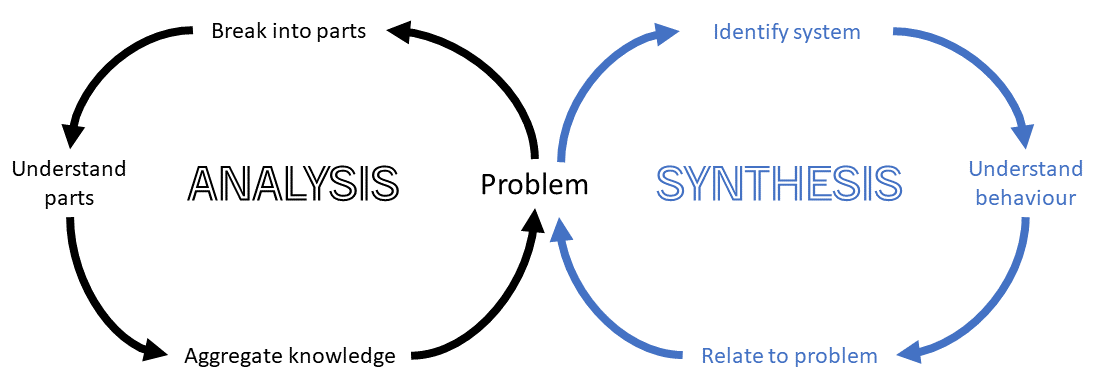
\includegraphics{./figures/Systems Thinking Defn Analysts.png}
	\caption[Why things happen][6pt]{Systems Thinking happens when you add Synthesis to Analysis Thinking. Synthesis seeks to explain why things happen, as opposed to analytical thinking, which focuses on constructing knowledge about what, when, where something is happening. The starting point for a systems inquiry is the question, what is this a part of? Understanding relationships that represent system causality allows for the further exploration of system behaviour.}
	\label{fig:stda}
\end{figure}

This approach is completely different to analytical thinking, because it does not seek understanding through a ‘reductionist scientific method’, but rather looks at challenges and problems as components of a wider system. This approach to problem solving seeks to understand the ‘whole system’ (cf. case study Appendices C, F and H). It is necessarily qualitative (or ‘soft’) when exploring what people think about the problem (often termed their hidden mental model).

System dynamics modelling, attempts to capture the developed shared-understanding of system structure in order to simulate the resulting dynamics of the system, potentially leading to greater knowledge about the system and enabling group learning. System modelling connects analytical thinking to the users of health intelligence in a useful way (cf. case study Appendices B, D, E, G). It allows them to explore the dynamics of quantitative knowledge in specific settings, eg. an ICS.

\subsection{Ackoff's definition of a 'system'}

Is it just something composed of other interrelated things, like your car, which is composed of parts: e.g. wheels, an engine, seats, a chassie, etc? Russel Ackoff liked to define a system in terms of the automobile, something most of us can relate to at some level. Who am I to argue with such a giant in the field of systems thinking?

An automobile is unlike any of its parts. You can drive a car. It carries you from one location to another and maybe some friends and your luggage/groceries/golf clubs or whatever you might be hauling about. That use or behaviour can't be found in any of the parts of a car. Only the car can carry you about. It is the system that moves you and stuff from place to place.

Your car has lots of parts, but from a systems point of view only some of them are essential parts of his system. However, even essential parts won't have an independent effect on the behaviour of the car. For example the engine provides the energy for motion, but is useless without the wheels to allow motion or a transmission and axels to connect the energy produced in the engine with the wheels. All of these essential parts have relationships with other parts, and are interdependent in terms of their effect on the system.

If, like me, you have taken your car apart to some extent (in an attempt at some repair undoubtedly), you will have noticed that your car was unable to perform its function in that state of disassembly. Its fundamental property, to move you and your stuff about the place, has disappeared. Therefore, while disassembled your car is no longer a system. It's just a lot of car parts cluttering your garage or driveway.

We only have a system (or indeed a car) when its behaviour differs from that of its parts. Although the systems we are interested in are predominately not mechanical, like cars, I find this to be a useful and far reaching analogy across all the systems of interest in public health practice:

\begin{itemize}[leftmargin=2cm]
	\item[organisms] systems with much greater complexity than your car, but the analogy holds and microbes, insect vectors, other animals of public health interest that might host pathogens or be hazardous in another way, and of course us (we are a special case due to this tricky concept called 'choice') are all composed of parts (most of which are essential) that depend on an interaction with at least one other part to to effect system behaviour
	\item[natural] systems are often separated into the major earth system components -- atmosphere, hydrosphere, geosphere, biosphere, and cryosphere, but ultimately there is only one earth system. We need to draw boundaries based on what problem we are trying to solve, therefore, we are often interested in parts of larger natural systems. Sometimes that might be a distinct ecosystems including soils and environmental microbiomes
	\item[social] systems include 'communities of people' (variously defined), organisations and what might be thought of as 'communities of organisations' defining healthcare, social care, or education systems for example (these can be tricky as the word 'system' is in common usage -- when you see it used as such ask yourself if it meets Ackoff's definition)
	\item[technical] systems of interest might include computing, transportation, utilities, essential public services, manufacturing and logistics -- their functioning impacts public health directly and indirectly by underpinning or influencing all other systems
\end{itemize} 

These 'types' of systems are offered to help you in your conceptualisation of systems, because most of the systems we are interested in are 'invisible' to those who are not looking. Donello Meadows famously said, "there is only one system", and because we can never deal with everything (think of the phrase 'boiling the ocean'), systems thinking requires us to conceptualise 'the system' in terms of the problem we are trying to solve.

%\section{Proactive Systems-Based Practice}
%\section{Think 'synthesis': Build proactive practice}
\section{Organisations also need to rethink their 'ways-of-working' and 'learning'}

Building a proactive public health means focussing on the structure and underlying worldviews that sustain our health problems. It consequently means moving away from our current near total focus on health events and their patterns.

\newthought{Current public health}: Through its intelligence and research functions, attempts to understand past health risk and outcomes in order to develop appropriate interventions that we hope reduces future risk and associated poor outcomes. Imagine driving your car on the motorway, with a completely blacked out windscreen. You are only able to anticipate traffic ahead by using your rear view mirror to watch the behaviour of traffic behind you, and near real time monitoring of the situation is only available by looking our your side windows. You cannot see further ahead than your side windows allow, so is it any surprise that you miss your exit and crash your car into the back of slower moving vehicles?

\newthought{Future public health}: Through its intelligence and research functions, creates accurate models of population health, and it uses these models to anticipate risks and outcomes before they occur, by understanding system behaviour. Imagine that you are on the same motorway in the same old car with a completely blacked out windscreen. Only now your car has two systems guiding it. System one is a self-driving capability that allows your car to know where it is at all times geographical and is able to sense cars immediately around it, enabling it to navigate to exits and to do this without crashing into other vehicles. System two provides a networked capacity to know what is happening throughout the road network so that it can anticipate and avoid the worst traffic. Just imagine.

%\section{Proactive public health practice transforms how we think about problems}
%\section{Systems-Based Problem Structuring}
%\section{Do system interventions: Manage problems}


Current analytical thinking practice is to deal with the problems we face one at a time, in isolation. To keep it simple. So we can understand it. Systems-based practice reframes identified problems into systems that contain the problem. The degree to which this facilitates successful management of the problem depends on how well we have identified the system containing the problem. A systems-aware public health practice is one that:
\begin{itemize}
	\item Moves from solving problems to managing problems
	\item Recognises that we face more than one 'type' of complexity
	\item Understands that shared-understand is a co-design process
	\item Understands that system intervention is a co-production process
\end{itemize}

\subsection{From solving to managing problems}
This is all about the structure of problems...

Ackoff has a lot to say on this subject matter -- managing the mess, also Theory of Constraints in the Goal, Checkland's soft systems work to develop shared-understanding on what problem we are trying to solve, etc.

\subsection*{Recognising complexity}

\subsection*{Shared-understand and co-design}

\subsection*{System intervention and co-production}




%\section{Transformative Systems-Based Public Health}
\section*{Learn together: Transform your organisation}

We talk a lot about transformation, transformative and transforming in public health and healthcare. Unfortunately, its mostly used simply as a synonym for 'change'. Or in some cases 'big change'. Transformation is defined as a change from one thing into something else. Anyone who's owned a kids toy called a Transformer, or seen the movies, knows what I'm talking about. Alien robots that transform into a completely different machine like cars, diggers or helicopters. Robot. Car. Not the same.

Systems-based public health can provide a transformative public health practice, because it:
\begin{itemize}
	\item Fundamentally shifts the way of working away from hierarchy and process into an Agile framework delivering co-design and co-production as a matter of course
	\item Humanises complex processes, relationships and organisations, which facilitates the changing of hidden mental models or worldviews
	\item Increases the scope of learning from individuals to organisations
\end{itemize}










This is a recounting of systems thinking that took place at Public Health Dorset, 2016-2020, a local public health system in South West England.

\subsection*{Mental models and co-design}
One of the fundamental aspects of synthesis thinking is that it can't be done in isolation -- unlike analysis thinking -- it requires as much perspective as possible. Synthesis thinking is literally 'team work'. It is defined by efforts to extract understanding from people. To share that understanding.

use of thinking tools

design thinking approach



\subsection*{System Dynamics Modelling}
Climate change model

Covid19 SEIR model


\subsection*{Preparing the future workforce}


\section{So now that we've seen the light, how do generate power?}

\chapter*{A Coherent Systems Practice \& Framework}
\addcontentsline{toc}{chapter}{coherent} 

\openepigraph{Leaders and managers face increasing complexity and uncertainty because technical, organizational, socio-cultural, political, and environmental issues have become intensely interconnected. Systems thinking is recognized as the essential competence for managing complexity. As the demand for systems thinking grows, however, the fragmentation of the field into different methodologies has become a potential liability.
}{Michael C Jackson}

\marginnote{
	\newthought{Key Takeaway:} It is not enough to 'do systems thinking'. There are too many disparate systems approaches. How do you know which approach is most appropriate? You won't, unless you have a methodology to do just that. Critical Systems Practice provides a cohesive systems-based practice providing just such a methodology. It provides organisations with the necessary structure for systems thinking, doing and learning.
}

\newthought{Increase the effectiveness of your organisation}. There are a lot of things you can do, but we can bundle them into three foci:
\begin{enumerate}
	\item Answer the 'right' questions
	\item Learn together as an organisation
	\item Aim interventions at improving system-outcomes
\end{enumerate}
The first idea shouldn't seem revolutionary, no one wants to waste time focussing on the wrong question. This is all about developing shared-understanding and it can only be done by working 'together'. I know, scary for some. On the plus-side it can be done effectively and efficiently in a virtual environment.
 
The second idea might sound a bit touchy-feeling, but I can assure you this is straight out of the systems dynamics play book and you should be thinking about simulation modelling. Of course it isn't only simulation modelling, but this is such a powerful tool for group learning you avoid it to your organisation's own detriment. However, all sorts of 'modelling' can be invoked -- conceptual, logical, graphical, etc. Your starting place depends where you are as an organisations, but you should be heading towards simulation modelling.

The third idea, if you read the previous two Chapters and didn't just skip to this -- what do I do Chapter, is really the most difficult and will take the most time to implement. This is why you need to get going almost immediately. Don't do what I've done and spend years developing the 'shared-understanding muscles' only to then start really thinking about how you are going to use them to change your system. And yes, system change, is what you are after. This is in essence a 'total quality management' approach to public health practice.

However, you aren't going to get very far if you are unable to bring anyone in your organisation along with you. You need to understand what you are up against.

%\section{From Ackoff's Stories to Jackson's Cohesive Approach}
\section{Arrival at 'New Thinking'}


What Ackoff does for 'Mindset' (at least for me), Michael C. Jackson does for 'structurally cohesive approach to problem solving'. In theA helicopter view of systems practice same way Ackoff deepened my understanding of what it means to use a 'systems perspective' to solve (or rather manage) problems, Jackson sets out a vast, and to me, and an undiscovered landscape of systems thinking with many differing perspectives. Confusion ensues. I found his magnus opus in 2019, and just wow.\cite{Jackson2019} A completely new picture of systems thinking, but dense and heavy with philosophy and social science theory, which I found both revelatory and hard going!

I had already been working on this book for a couple years, when I discovered Jackson's tome. I learned a few things over the next couple of Pandemic-years: 
\begin{enumerate}
	\item As I've said before, I found that I was working with a very restricted view of what systems thinking is or could be (not to worry, I was finding out rapidly that most of my colleagues were in the same boat -- indeed most of them hadn't and still haven't gotten beyond systems dynamics!),
	\item that most of the academics involved in pushing or developing particular systems thinking approaches are more interested in their own world view than they are in helping you, a practitioner, understand how to use it successfully, and
	\item as a consequence their use of language seems to make all of this harder than it ought to be. Their competition for recognition within their respective communities is not helpful to people like you and me, nor is it helping the public sector to adopt this paradigm(s) of thought.
\end{enumerate}

And yet... And yet, despite their best efforts to remain esoteric, which in my experience was exceptionally successful, I was able to understand enough of what Jackson was talking about to understand that you could put a structure around these many divergent efforts to look at the world from a systems perspective. Jackson labels these system-of-systems methodologies or "second-order" methodologies that provide a 'critical' pathway into understanding how all these systems approaches fit together.

\subsection*{Critical Systems Practice -- EPIC}
Jackson's magnus opus and his follow-up practitioner's Guide"\cite{Jackson2024} present Critical Systems Thinking as culmination of the system-of-systems approach. He structures this second-order systems practice approach around a continuous process of critical reflection involving: Explore -- Produce -- Intervene -- Check (Figure~\ref{fig:epic}), which maps out the over-arching methodology of Critical Systems Practice.

\begin{figure}
	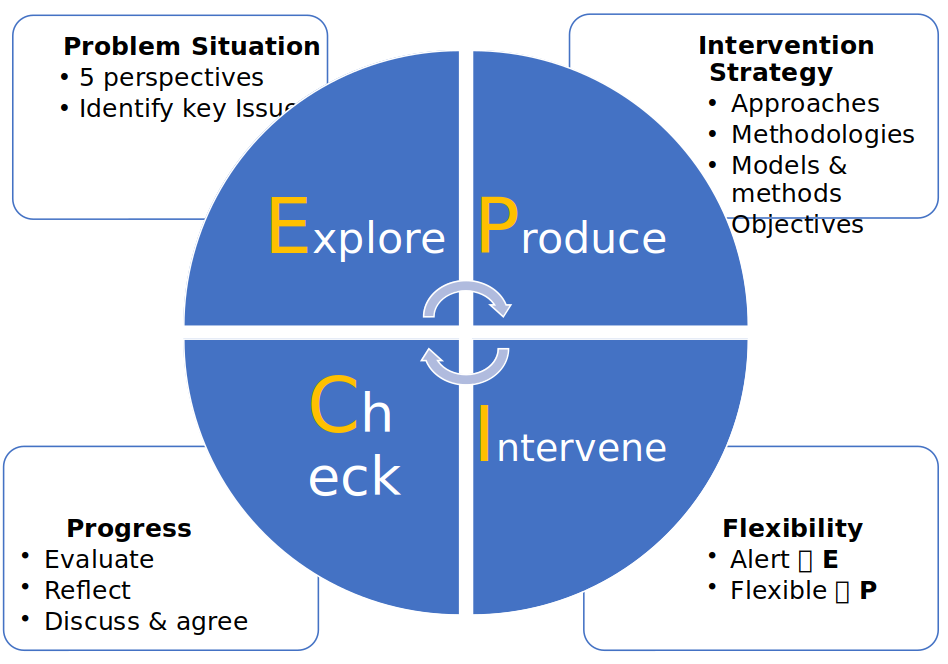
\includegraphics{./figures/epic.png}
	\caption[EPIC -- Critical Systems Practice][6pt]{Critical Systems Practice is implemented through Jackson's EPIC or Explore -- Produce -- Intervene -- Check [Obviously, like many of my diagrams it needs to be redrawn, but it is a good enough placeholder!].}
	\label{fig:epic}
\end{figure}

However, I found his very simple idea (the one he uses to organise the first of these two books), that we can group all methodological approaches into six types or sources of complexity to bring much needed clarity to the systems landscape (Table~\ref{tab:sysapproaches}). Against this classification of complexity, he maps 12 major systems methodologies.

\begin{table}[h]
	\begin{center}
		\footnotesize%
		\begin{tabular}{p{3.5cm} p{6cm}}
			\toprule
			Complexity Challenge & Systems Approaches \\
			\midrule
			Technical Complexity & Operational Research\linebreak  Systems Analysis\linebreak Systems Engineering \\
			Process Complexity & The Vanguard Method \\
			Structural Complexity & System Dynamics \\
			Organisational Complexity & Social-Technical Thinking\linebreak Organisational Cybernetics \\
			People Complexity & Strategic Assumption Surfacing and Testing\linebreak Interactive Planning\linebreak Soft Systems Methodology \\
			Coercive Complexity & Team Syntegrity\linebreak Critical Systems Heuristics \\
			\bottomrule
		\end{tabular}
	\end{center}
	\caption{Matching system problems to approaches, after Jackson 2019}
	\label{tab:sysapproaches}
\end{table}





%\section{Get buy-in \& build a coalition for change}
\section{If you don't build it, where will the change come from?}


Who is in the market for systems-based public health practice? This is a much different question from who is going to be open to systems thinking ideas -- or almost any new ideas about how to go about something.

Much earlier in my career I read a book on marketing called \emph{Crossing The Chasm}, because I was looking at the challenge of introducing disease spread simulation into public health practice\sidenote{Moore GA. Crossing the Chasm: Marketing and Selling Technology Products to Mainstream Customers. Second Edition. 2004. Capstone. Pages 211.}. I was finding people who were interested. They were everywhere, but they were few in number. Often they were people who were interested in everything, they liked ideas, they liked to play with ideas and to share these ideas. It was always wonderful to find these like minded thinkers!

\emph{Explore}: Problem situation. Examine the situation using five systemic system perspectives: (1) mechanical, (2) interrelationships, (3) organismic, (4) purposeful, and (5) societal/environmental.

\emph{Produce}: Intervention strategy.

\emph{Intervene}: Flexibly.

\emph{Check}: Progress. 

However, as I found out, there is a problem with these like minded thinkers. As Moore's book points out, I'd just learned what innovators are, or at least what some innovators (myself included) are like. We are the first to embrace new ideas, we create pilot projects, we agitate to try x, y and z. Sometimes it catches on sometimes it doesn't.

Moore identified five segments in his "revised technology adoption life cycle". Five segments to conquer -- in public health practice as in anywhere else these are the Innovators, Early adopters, Early majority, Late majority, and Laggards (NEED A MODIFIED FIGURE).

The literature on systems thinking in public health suggests we are now into the early adopters phase. We have more pilots than British Airways (you have no idea how long I've been waiting to use that joke). A select group of people in public health organisations all over the world are putting systems-based public health practice to the test, yet we have not 'crossed the chasm' and we have not moved beyond pilot project tests.

CLIENT CENTRED TRAINING? GREAT PLACE FOR THEIR ENGAGEMENT FIGURE?

\subsection{Never let a crisis go to waste}
Crises, minor panics, tough spots -- these are all natural breaks where for a short period of time people are willing to accept that what they have been doing is no longer working. This happens for a million different reasons. It might not even be declared as such, but they happen and you need to know what they look like in your organisation.

\subsection{Start with your analysts}
There is a clear, but largely unexplored path with your analysts -- if you can seed systems thinking into this group you've created an engine room of problem solving facilitation.

\subsection{Choose your clients carefully}

\subsection{Who should be invited to participate?}

\subsection{Not crisis -- opportunity}
Act when you have their attention. Sometimes it is the only way forward.

\subsection{Picking a good client to get started}


% Place holder Section as I build a readable ToC
%\section{Implement new ways of working}
Agile together, humanise the workplace, as part of 'the system'
% Place holder Section as I build a readable ToC
%\section{Doing: Apply shared-understanding to change systems and manage problems}



% Place holder Section as I build a readable ToC
%\section{Learning: Deepen shared-understanding to create organisational learning}
\section*{Make it work}
\begin{itemize}
	\item move from expert to facilitator thinking, doing \& learning
	\item replace 'solution' thinking with 'management' thinking
	\item model problems to improve decision-making
\end{itemize}

%\subsection{If you don't know what to expect, how will you know it if you've achieved it?}
The goal is to move public health practice from its 'Hail Mary' approach to setting goals and expectation to a more informed and managed process that improves organisational shared-understanding. There are a number of ways we can do this.
\begin{enumerate}
	\item Logic modelling
	\item Graphical modelling
	\item Simulation modelling
\end{enumerate}

\subsection{System dynamic modelling}

\subsection{Organisational learning -- future directions}


\section{The messy bits that don't work well in top-down management structures}



\chapter*{Introduction}
\addcontentsline{toc}{chapter}{Introduction} 

\openepigraph{The reasonable man adapts himself to the world: the unreasonable one persists in trying to adapt the world to himself. Therefore all progress depends on the unreasonable man.}{George Bernard Shaw, Man and Superman}


\newthought{This} wasn't the book I had intended to write. After many years working in public health intelligence (PHI), and being increasingly frustrated with my inability to determine if I was making a difference, I began looking for better ways of delivering 'intelligence'. I eventually found 'systems thinking', although not right away, and this book was going to be about my learning journey into systems thinking. The focus was going to be:

\begin{itemize}[leftmargin=1 cm]
	\item My problems, as an analyst, in trying to deliver PHI,
	\item Improving the practice of public health intelligence, and
	\item Produce a user guide for colleagues in my organisation. \end{itemize}

At some point, I embraced this writing project as part of a much wider learning journey that included many colleagues. I've lost count of how many times I've stopped and restarted this writing project. What started as a modest user guide has become a much bigger writing endeavour reflecting the length of our learning journey. This isn't just about me, the analyst, or public health intelligence as a function within public health. I'll explain why later, but this about all of collectively being more effective: Public health intelligence colleagues, public health colleagues, Civil Service colleagues, and especially wider public sector colleagues.

However, before I got to this point there were at least four years of pushing forward and repeatedly running into a wall. Sometimes I had to go back to double check my facts (a lot of that), sometimes I was re-evaluating whether I really believed what I had just written, but mostly it was because what I was writing sounded a bit hollow (maybe readers will still think that). Hollow in the sense that I didn't feel I had any direction to give, even after years of trying to incorporate systems thinking into what I was trying to do.

In retrospect, this project feels like I've been peeling an onion for decades. I was looking for something simple (in all the wrong places), direct and user-guide-ish. So, I got out a knife, and peeled that first layer off. It wasn't looking like a systems thinking user guide at all. I thought I knew what systems thinking was all about, but I hadn't really scratched the surface.

\section{The Progress of Public Health Practice}
I've definitely been an unreasonable man most of my adult life, and my unreasonableness has grown with age and experience. That's not to say that public health hasn't progressed in its thinking, of course it has, but just not by leaps and bounds.

For example, if you are one of my public health colleagues you already know that public health practice is often referred to as: \begin{quote}
	The science and art of promoting and protecting health and wellbeing, preventing ill health, and prolonging life through the organised efforts of society.\sidenote{Faculty of Public Health (fph.org.uk), as of 14 July 2025.}
\end{quote}
As good a definition of our aims as any discipline could have done in so few words. However, what fewer colleagues will know that this quote originates from 1920: 
\begin{quote}
	The science and art of preventing disease, prolonging life, and promoting physical health and efficiency through organized community efforts for the sanitation of the environment, the control of community infections, the education of the individual in principles of personal hygiene, the organization of medical and nursing service for the early diagnosis and preventive treatment of disease, and the development of the social machinery which will ensure to every individual in the community a standard of living adequate for the maintenance of health.\sidenote{Charles-Edward Amory Winslow, an American bacteriologist, 1877-1957.}
\end{quote}
While wordier than our contemporary version, and perhaps without explicit consideration of mental health, it is clear that our aims have remained the same for more than 100 years. Our ambition  remains largely unchanged.

What about our methodology and approach to achieving these aims, have they progressed? I am going to argue that no, we are essentially approaching population the same way we always have. Without a doubt we are now far more technically, scientifically and analytically savvy, and our social views have also evolved, we have been making methodological progress. Nonetheless, our approach overall remains the same, epidemiology, often referred to as the science of public health, still follows the same principles of reductionism, as have most of the sciences.

While we have advanced our sciences to enable deeper and broader understanding of new diseases, forms of ill health, and medical technologies, we no longer appear to be enjoying the same level of achievement vis a vis our aims. Our populations no longer getting healthier each year, progress has slowed and even reversed in some regards. To be sure, our populations are longer lived than they were in 1920, but for how long?

This book is about effectiveness in public health practice and what I, and many colleagues, believe we need to change about our approach if we are to recapture the early progress of our discipline of public health. Furthermore, I am going to suggest how we and our organisations need to change our practice in order to improve effectiveness. You may indeed see this as unreasonable, and you wouldn't be the first of my colleagues to suggest this.

\section{My Personal Journey}
I'm going to relay to you some of my career story and public health experiences, which will probably be different from yours. Nonetheless, I hope it will encourage you to reflect on your career experiences areas of interest, as have I, in order to see them in a new light. I think that this can be a more powerful way of launching your own systems learning journey.

I started questioning my approach to and the value of what I'd been doing in public health intelligence for more than a decade. Data driven organisations. Information for action. Is it just me, or do public health (maybe even public sector) inteventions less effective and less impactfull that they used to be? At the very least, I can't see changes in interventions, decision-making or population health outcomes as a result of the work my colleagues and I deliver.

The questions I've been asking are:
\begin{description}
	\item[Impactfulness] Are our, in the widest public sector sense, interventions having an impact? I honestly don't know, but it feels like we aren't having as much of an impact or as consistent an impact as we might have in the past. I'll take you through what public sector leaders are saying about this though, and spoiler alert, many colleagues believe that rising levels of complexity are at the root of the problem.
	\item[Workforce Effectiveness] Does this meant that we (public health intelligence analysts, the wider public health and public sector workforce) are also not being as effective as we once were? Are we happily lingering in the tepid bath of decline, as one British Prime Minister recently suggested? If this means that we are locking into a single problem solving paradigm of reductionist scientifically based analysis, then yes, we might just have to change how we approach problematic and complex situations in the public sector.
	\item[Systems Thinking] I've heard, and you have too or you wouldn't be here, that there is this thing called systems thinking that could be put into practice that might help us improve our effectiveness and impact within the public sector. It does mean that we have to adopt a new way of working and thinking. This will take some considerable effort on our part, but what other option do we have?
\end{description}

This book is really about trying to answer these and loads more questions that I've been asking myself and responding to some of the many challenges from colleagues. The push-back has comes in various guises, but it seems to have three components:
\begin{enumerate}[leftmargin=1 cm]
	\item Analysis produces the only acceptable evidence-base,
	\item The resulting scientific evidence-base underpins modern public health practice, and
	\item There are no acceptable alternatives to informing practice.
\end{enumerate}
Consequently, some colleagues will argue that we must focus all efforts on improving analysis by adopting more data science methods, including the use of large language models, and moving from analysis to analytics to automate analysis processes, e.g. producing dashboards -- in short, we just need to do our jobs more efficiently in order that we have a bigger impact.

Thus we have a social norm for analysts (maybe most of the public sector workforce) of all stripes, not just public health intelligence analysts, that the reductionist scientific process of analysis produces the only acceptable evidence-based. Challenging this deeply ingrained belief turns out to be a huge challenge in the public sector, maybe even "unreasonable", besides which it will take too long and we don't have enough resources to satisfy the analysis requests.






% Part I: Population Health Complexity
\part{Population Health, Complexity and Systems}

\chapter{Evolving Population Health Challenges}%

\openepigraph{Why treat people and send them back to the conditions that made them sick?}{Michael Marmot}

\marginnote{
	\newthought{Key Takeaway:} Complexity is making public health less effective than it might once have been and it is seen to be less effective. Our inability to step outside our analysis paradigm is, I believe largely responsible for the situation. It has become so ingrained it is 'thinking', and we compound the ways-of-working that make it ever more difficult to escape. 
}

\newthought{Complexity}: Whenever I talk or present on the subject of complexity, I am reminded of Dune, a Frank Herbert created universe in which its Bene Gesserit repeat the above as a litany against fear. Subconsciously, I insert 'complexity' after 'fear'. I can hear an inner voice saying it... There is no other public health topic that provokes such strong aversion. It really is a mind-killer! The public, colleagues, politicians -- almost everyone will walk a long road to avoid having to deal with it.

It would be hard to argue that our world isn't complex; and, I have yet to ever hear a colleague state that they would like their organisation to be less effective. These are modern day 'motherhood statements'. Almost everyone would agree, and almost no one seems to be doing anything about it. It is easier to agree with this statement than it is to understand the implications. Maybe the key sticking point is the word 'requires'.

Complexity 'requires' more effective practice. Does it? Why? What is wrong with the current practice of public health? Well there are a couple things wrong. First, our practice is 'reactive' -- we see events (deaths and illness) and then we react to their occurrence. Secondly, we focus on the event itself and we rarely explore why the event occurred beyond the most proximal causes. Thirdly, and most bizarrely, we treat almost every illness as if it was a 'stand alone' problem, not at all related to any other form of ill health. In fact, we've organised not only public health practice around this idea, but our health systems and even the study of medicine are organised into disease specific silos. 

If effectiveness is the degree to which your organisation achieves its desired outcomes or results, who wouldn't want their organisation to deliver more effective public health? I've never worked in a public health organisation that couldn't have achieved more than it was actually delivering. If '0' represents achieving nothing (zero effectiveness) and '100' achieving everything (perfect effectiveness) -- how do you rate your organisation?  

Typically, a public health organisation's approach to being more effective is to attempt new types of intervention, or if it all seems to be getting a bit desperate we'll restructure our organisation or even our health system! So we already expend a lot of resource on trying to be more effective. How's that working out for your organisation? It seems a bit hit and miss, doesn't it? Moreover, this doesn't address the key limitations of current practice: reactiveness, proximal focus and silo view of the world.

If you are a colleague interested in public health outcomes, this book will help you understand how to identify effectiveness gains and build them into the fabric of your organisation. This is nothing less than transforming the way organisations think, do and learn. I hasten to add that I'm not advocating burning-the-house-down and rebuilding, but rather about modernising the old property by putting in a new windows so that we can see more of the outside and let more light in.

\section{A journey into health systems complexity}

In the mid-1980s, years before I knowingly found my 'public health' career path, I landed an incredible summer government internship monitoring agricultural pesticides in the ground water of Southern Ontario, Canada. It was incredible, because it had everything: It used almost everything I was learning in my Geography undergraduate programme and it provided a real world application of all this learning. I thought that was pretty cool, and I knew I was very lucky. After many years of hospitality jobs, I was doing something that I felt for the first time could be the start of a career path! Not only that, they gave me a car, there was an expense account for lunches, and all I had to do was drive around in the sun with the windows down, the radio turned up and visit my list of farms each week over the summer and take a sample of water from an outside tap.

This 'first real' job, as I felt back then, has long dropped off my CV. I would only remember the fun I had these many years later, were it not for the fact that my boss at this government agency encouraged me to do the research year of my honours degree on the programme I was working for, so my very first real job is documented by my 79 page, leather bound 'undergraduate dissertation'. No one has ever cited this research to my knowledge, so let me be the first\cite{Skelly1988}.

The monitoring programme ended up running for three or four years, but  because of the concerns it began to generate. The first summer, and the one I based my undergraduate thesis on, had not identified the target pesticide, Alachlor nor its metabolites, and we only had a few regularly positive wells for the most widely used pesticide Atrazine and it's metabolites. Consequently I went with the flow and took a slightly wider focus for my academic research: 

very few wells that we monitored showed any contamination, but many more wells were found to be contaminated during the second summer. By the third summer most wells were contaminated. 

We were sampling drinking water wells on farms and, as you can imagine, this was a 'problematic situation' to put it mildly. These wells were largely defined as being shallow and in unconsolidated sand and gravel aquifers. Exactly the type of wells that you would expect to see pesticide contamination in if the pesticides were getting into the soils and down into the groundwater. 

However, what you really need to know was that this didn't seem to be related to the introduction of new pesticides or any change of practice on farms relating to how pesticides were sprayed, when they were sprayed or how the soils were fertilised or ploughed. The crop cover was largely static. Nor did it seem that changes in rainfall could explain the changes. Blame complexity.

In fact, when we started seeing more wells contaminated in the second summer, it was well understood what was happening. The problem happened before the groundwater sampling for pesticides even began.


\begin{itemize}
	\item (1) complexity is killing us; (2) it's largely down to our analysis (reductionist) mindset; (3) and public health's lack of diversity (do I really believe this last issue is a separate issue or just a factor in analytical thinking?)
	\item Public health is the proverbial frog in a slowly heated pot of water. It is an existential crises.
	\item Having a sound analytical framework and narrow range of thinking within the public health profession has limited our scope of action in dealing with a changing environmental situation, eroding our effectiveness...
	\item our lack of diversity: same management structures and problems, ie.'just do it' do it mentality; same education; dominated by biomedical model; where are the engineers?
\end{itemize}

\section{Public health through the ages}

\section{Science-led public health}
In the mid-19th century, public health issues were often perceived as linear problems with straightforward solutions. The Cholera Epidemic of 1854, for instance, was initially thought to be caused by miasma (bad air). Dr. John Snow's groundbreaking work in identifying contaminated water as the source marked a shift towards more evidence-based approaches in public health. 

As we moved into the 20th century, public health challenges became increasingly complex. The establishment of the NHS in 1948 represented a systemic approach to healthcare, addressing multiple health issues simultaneously. This shift recognized the interconnected nature of health problems and the need for comprehensive solutions. 

The latter half of the 20th century saw the emergence of even more complex challenges. The HIV/AIDS epidemic of the 1980s, for example, required not just medical interventions but also social and behavioral changes. This highlighted the multifaceted nature of modern public health issues. 

In the 21st century, we face highly complex, interconnected challenges like the obesity epidemic and climate change-related health issues. These problems involve multiple systems - social, economic, environmental, and biological - interacting in complex ways. The COVID-19 pandemic further emphasized the global interconnectedness of health issues and the need for coordinated, systemic responses. 

This evolution from linear to complex challenges necessitates a shift from reductionist thinking to systems thinking in public health. The table provides specific examples that illustrate this progression, offering a valuable resource for your book section.

\begin{table}[h]
	\centering
	\caption{Chronology of some key modern population health events and their significance from a UK perspective.}
	\begin{tabular}{@{}p{0.22\textwidth}p{0.73\textwidth}@{}}
		\toprule
		\textbf{Events} & \textbf{Public Health Significance} \\
		\midrule
		Cholera Epidemics 1831-1854 & \emph{On the Mode of Communication of Cholera}: John Snow identified waterborne disease, marked shift to evidence-based public health and an 'origin story' for epidemiology.
		\\
		Chadwick's Report 1842  & \emph{Sanitary Conditions of the Labouring Population}: Linked poor living conditions and disease, leading to 1848 Public Health Act.
		\\
		Universal childhood vaccination 1840s & From Edward Jenner's 1796 smallpox vaccination followed widespread success including diphtheria 1940, pertussis and tuberculosis 1950, polio 1956, measles 1968, MMR 1988, HPV 2008.
		\\
		The Great Stink 1858 & Redevelopment of London's sewage system, provision of council sanitation services, Medical Officers of Health: 1875 Public Health Act.
		\\
		Influenza Pandemic 1918-19 & There were close to 250k UK deaths and 50-100 million deaths globally. Initial response was slow and uncoordinated: school closures, public gathering ban, quarantine, isolation - emphasis on ventilation and disinfection.
		\\
		Establishment of NHS 1948 & Introduced universal health coverage, emphasizing access and equity. Provided a single coherent system of health services for the first time. Measurably increasing population health.
		\\
		Post-War Slum Clearances & Improved living conditions by relocating people to modern homes with green spaces: New Towns Act 1946, Housing Act 1956.
		\\
		London's Great Smog 1952 & This deadly smog event killed an estimated 12,000 people highlighting the urgent need for air pollution control for coal fires leading to the Clean Air Acts of 1956 and 1968.
		\\
		Tobacco Control 1964 &	Sustained public health campaigns against tobacco use and implementation of restrictions from 1965 Television Advertising Ban through 2024 Tobacco and Vapes Bill.
		\\
		HIV/AIDS Pandemic 1981 onward & Emerging infectious disease revealed interplay between health, social behaviour, and stigma. Focus on sexual health education and significant advances in anti-virals.
		\\
		Obesity Epidemic 1990s & Interplay between individual behaviour, social determinants, and environmental factors prompted public health campaigns focused on nutrition and physical activity.
		\\
		COVID-19 Pandemic 2020-21 & With UK deaths exceeding 230K, weaknesses in global preparedness, and a lack of coordinated responses were identified. Accelerated mRNA vaccine technology development. A multi-year British Commission has begun hearings.
		\\
		\bottomrule
	\end{tabular}
\end{table}



\chapter{Understanding Population Health Complexity}
\openepigraph{Conceptually, the theory of epidemiologic transition focuses on the complex change in patterns of health and disease and on the interactions between these patterns and their demographic, economic and sociologic determinants and consequences.}{A. R. Omran, 1971}

\marginnote{
	\newthought{Key Message:} Complexity is making public health less effective than it might once have been and it is seen to be less effective. Our inability to step outside our analysis paradigm is, I believe largely responsible for the situation. It has become so ingrained it is 'thinking', and we compound the ways-of-working that make it ever more difficult to escape. 
}

\newthought{epidemiological transitions} are crucial concepts and the last one especially so because it marks the point at which we lost almost all of our effective tools -- they were useless against the rising tide of chronic disease. Sometime after the Second World War, maybe the 1960s, and it seemed that we had almost conquered infectious disease, public health turned its attention to chronic diseases (often termed 'non-communicable' diseases).

The emphasis went from doing, from engineering, from physical interventions as the way to deliver results -- to the processing and sharing of information and knowledge. The 'new' enemies are cancers, cardiovascular diseases including stroke and diabetes, chronic respiratory diseases, dementia, mental ill health, musculoskeletal disorders, immune system dysfunction, substance abuse, and many others, which are all influenced by the
\begin{itemize}
	\item Environment: air, water and noise pollution, weather and climate, nature and biodiversity, food system
	\item Conditions of living: local economy, economic resources, meaningful employment, housing availability, security and quality, public safety and crime, education and opportunity for development
	\item Lifestyle \& behaviours: social networks, family, substance abuse, exercise, stress, diet, sleep
\end{itemize}

I have been pondering three fairly fundamental questions of the 'practice of public health' that I'd like the reader to consider. How do we:
\begin{enumerate}
	\item Build a more effective systems-based \emph{Public Health} practice?
	\item Enable new ways of working that lead to more effective practice?
	\item Reimagine our system of learning beyond individual continuing professional development?
\end{enumerate}




\chapter{Analytical Constraints to an Evidence-Based Approach}
\openepigraph{The \emph{analysts} have only interpreted the world, in various ways.\linebreak The point, however, is to change it.}{after Karl Marx}

\marginnote{
	\newthought{Key Message:} 
}

Public health intelligence has two fundamental challenges: (1) Identifying the right questions, often generated elsewhere in the organisation and (2) answering these questions. We've not made significant advances on these two challenges over the 25 years or so that I've been involved in public health intelligence. The reason, in words attributed to Albert Einstein, is that

\begin{quote}
	\centering 
	\emph{We cannot solve our problems}\\ 
	\emph{with the same level of thinking that created it.}
\end{quote}

We have only one intelligence process that is widely used and that is 'analysis'. All modern evidence-based health and care systems are designed, run and supported using this fundamental process. If we are going to have any chance of tackling our two key intelligence challenges, we need to rethink our approach to problem solving.


\subsection{Rethinking Our Approach}

I believe that a mature intelligence function, in any type of organisation, should support critical problem-solving wherever that happens within an organisation or even across health and care systems. Intelligence processes need more depth; they need to be able to directly address the our key challenges. I propose the use of three interdependent problem-solving approaches be adopted by the organisational intelligence function (Table~\ref{tab:response}).

\begin{table}[h]
	\begin{center}
		\footnotesize%
		\begin{tabular}{p{1.75cm} p{2.75cm} p{4.75cm}}
			\toprule
			Intelligence processes & Problem-solving approaches & Principal output \& outcome for each problem-solving approach \\
			\midrule
			Analysis    & Analytical Thinking & Provide operational information\\
			& & Improved Knowledge \\
			Synthesis & Systems Thinking & Identify and frame critical problems \\
			& & Shared-understanding of why problems are occurring now \\
			& Futures Thinking & Compare multiple strategic directions \\
			& & Shared-understanding of routes to the most desired future states \\
			\bottomrule
		\end{tabular}
	\end{center}
	\caption{A layered approach to problem-solving in public health intelligence would include Synthesis, which provides two additional approaches.}
	\label{tab:response}
\end{table}

Public health intelligence might be unique practice within our health system for having no academic home, no single discipline. The fact that public health analysts are drawn from many disciplines is a strength when building teams, because intelligence groups are in general less vulnerable to disciplinary blind spots, which is why I think that intelligence functions should be about more than data, information and knowledge. Any small group with a plurality of perspectives should be thought of as organisational problem-solving facilitators. More on that later, but intelligence functions are a natural home for organisational process of synthesis (Figure~\ref{fig:apptosensemaking}).

\begin{figure}
	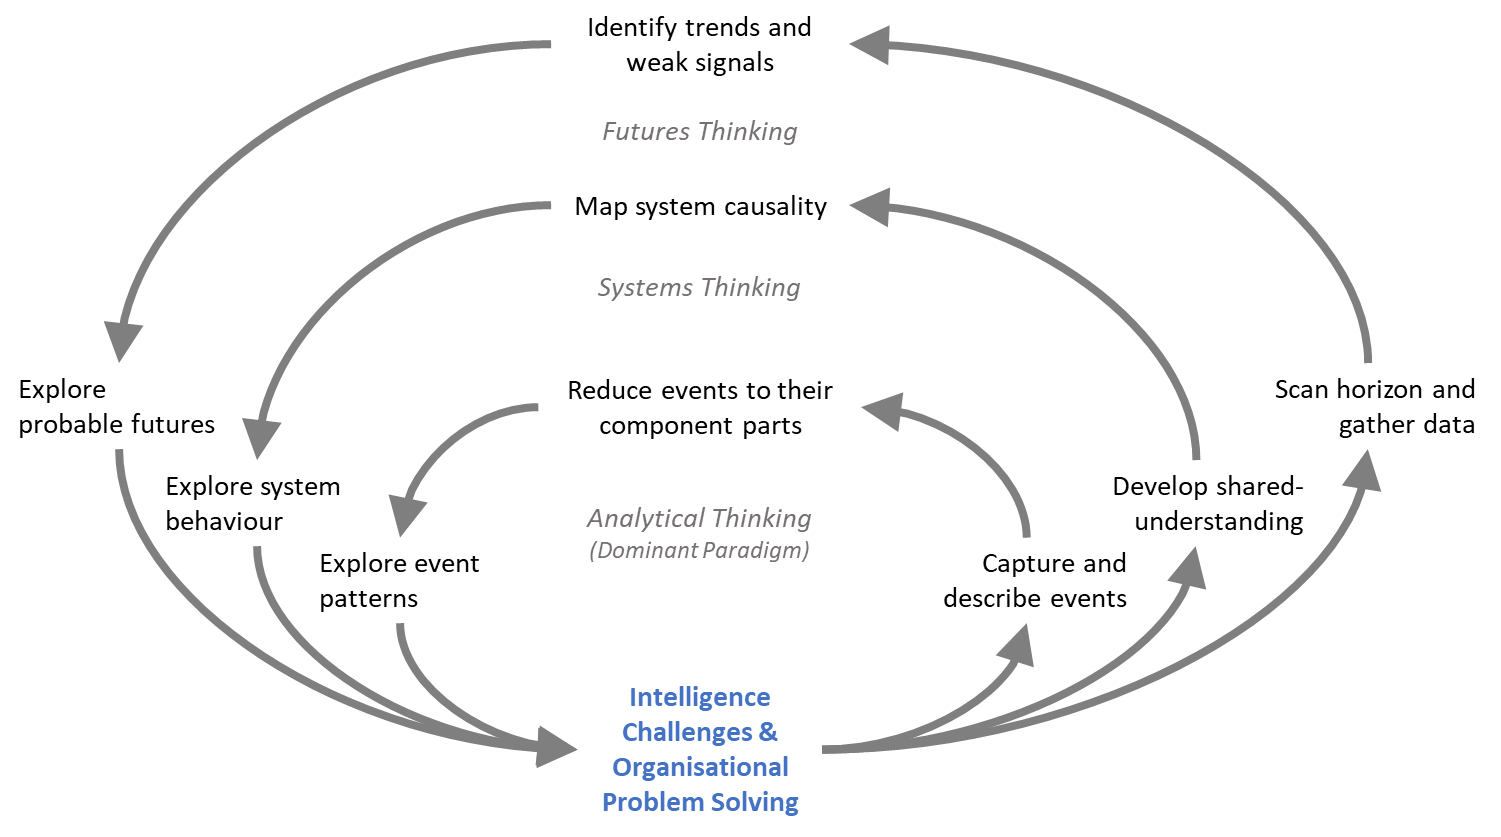
\includegraphics{./figures/approaches.png}
	\caption[Systems and Futures Thinking][6pt]{Systems and Futures Thinking, missing from all but the most mature intelligence programmes, effectively deepen the problem-solving capability of an organisation, by directly addressing the two key intelligence challenges. }
	\label{fig:apptosensemaking}
\end{figure}

My theory-of-change for the intelligence function itself suggests that if we transition our problem-solving from a single approach to three interdependent approaches we will ultimately increase the effectiveness of any public health organisation or health and care system of which we are a part (Figure~\ref{fig:toc}). While this premise is straight-forward, the purpose and implementation of these additional capabilities is a longer journey that I hope many of my colleagues will be keen to explore with me.

\begin{figure*}[h]
	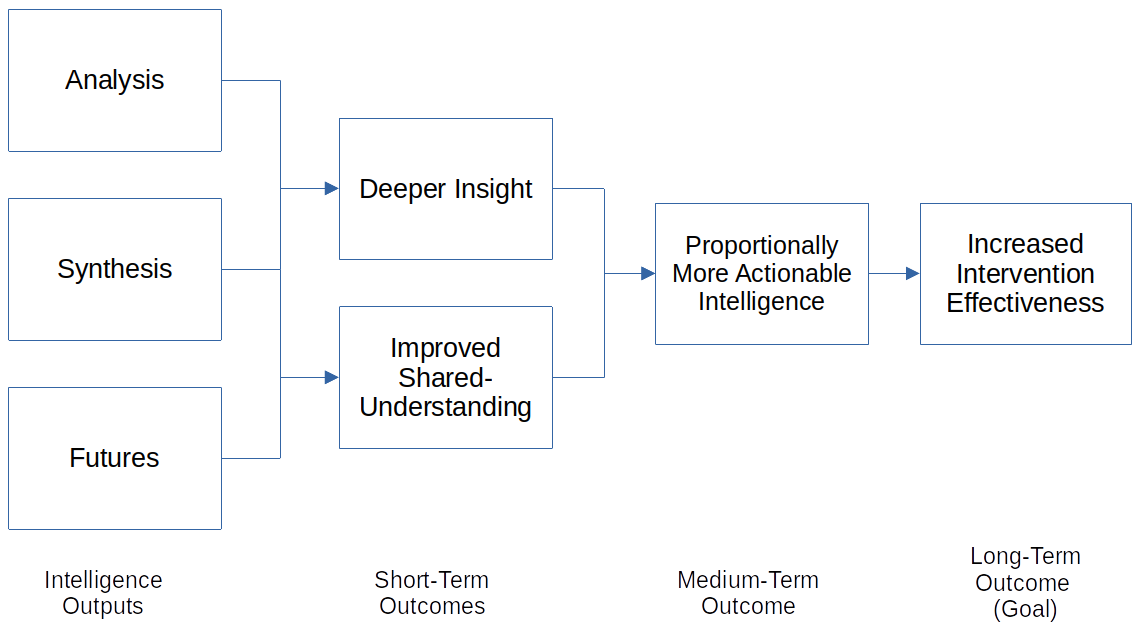
\includegraphics[width=\linewidth]{./figures/toc.png}%
	\caption{The premise underlying this book is encapsulated in this very simple theory-of-change. This same premise should underlie every mature intelligence process.}%
	\label{fig:toc}%
\end{figure*}


\section*{A public health intelligence perspective on the need for change}
I am a scientist by training and a public health intelligence 'analyst' by profession. I have managed a broad and varied career with work experiences across public and private sector organisations, including academia since the 1990s. I've lived, studied and/or worked in the United Kingdom, Australia, New Zealand and Canada with a few health intelligence projects in less resource rich nations. Public sector roles have included national, provincial/state, and local system work: Mostly in public health intelligence Teams, but also in biosecurity and environmental health teams.

In my, more limited, private sector experience of organisations, most if not all organisations are similarly ineffective, or at least less effective than they otherwise could be. Consulting work I have delivered into every type of organisation from non-governmental to trans-national corporation suggests to me that all organisations struggle to be effective. This is not just a public health organisation problem.

Nonetheless, sitting within Public Health Intelligence Teams has provided me with a privileged perspective into the challenges faced by colleagues across public health and associated organisations. We have, for as long as I've been involved, maintained a form of 'client-based' relationship with the rest of our colleagues. They ask questions; we provide answers.

Over the years I've noticed that we are pretty good at answering those questions and each year seems to bring some improvement, usually an 'efficiency', to our processes. I used to think that this was a good thing. However, the more I learn about 'systems' and how they produce 'system outcomes', the more questions I have. So many questions. However, the key one for me at this point in my journey is how do we better define and frame the problems we are trying to solve in public health -- so that we ask and answer the right questions?

Russell Ackoff used to repeat this memorable aphorism: Improving your answer to the wrong question, makes you wronger. Think about that for a moment. Really. Stop reading, look out the window and think about this statement for at least two minutes. The better (quality, detail, depth, etc) your answer, the wronger you become. So it is better (at least initially) to have the wrong answer to the right question, because improving your answer will eventually bring you closer to solving the right problem. 

Conversely, if you are focussed on solving the wrong problem, without any method of 'seeing' what is happening, you have no path back to the right problem. Anyone else see this happening? This happens because it is very difficult to see that we are working on a 'wrong' question/problem, due largely to the fact that lots of 'experts' support this identification. Naturally, many people defer to experts. I think this is where a lot of our problems arise.

\section{The mess in which we now find ourselves}

\section*{Why preventing ill health seems beyond our ken}
Analysis works! Analysts engage with clients to ensure that they are providing a useful answer client questions -- the previous figure outlines this process. We do this to ensure that public health interventions are supported by the best data and analyses available.

The Englightenment, a period beginning mid-seventeenth century, is an important milestone in development of modern science and with it the 'analysis' paradigm underpinning public health intelligence today\cite{Grant1997}.

The recording of deaths in London was taking place from the early 1600s and reported through the \emph{Bills of Mortality}, which recorded the occurrence of plague and other causes of death  (Figure~\ref{fig:billsofmortality}). 

\begin{marginfigure}[-15cm]%
	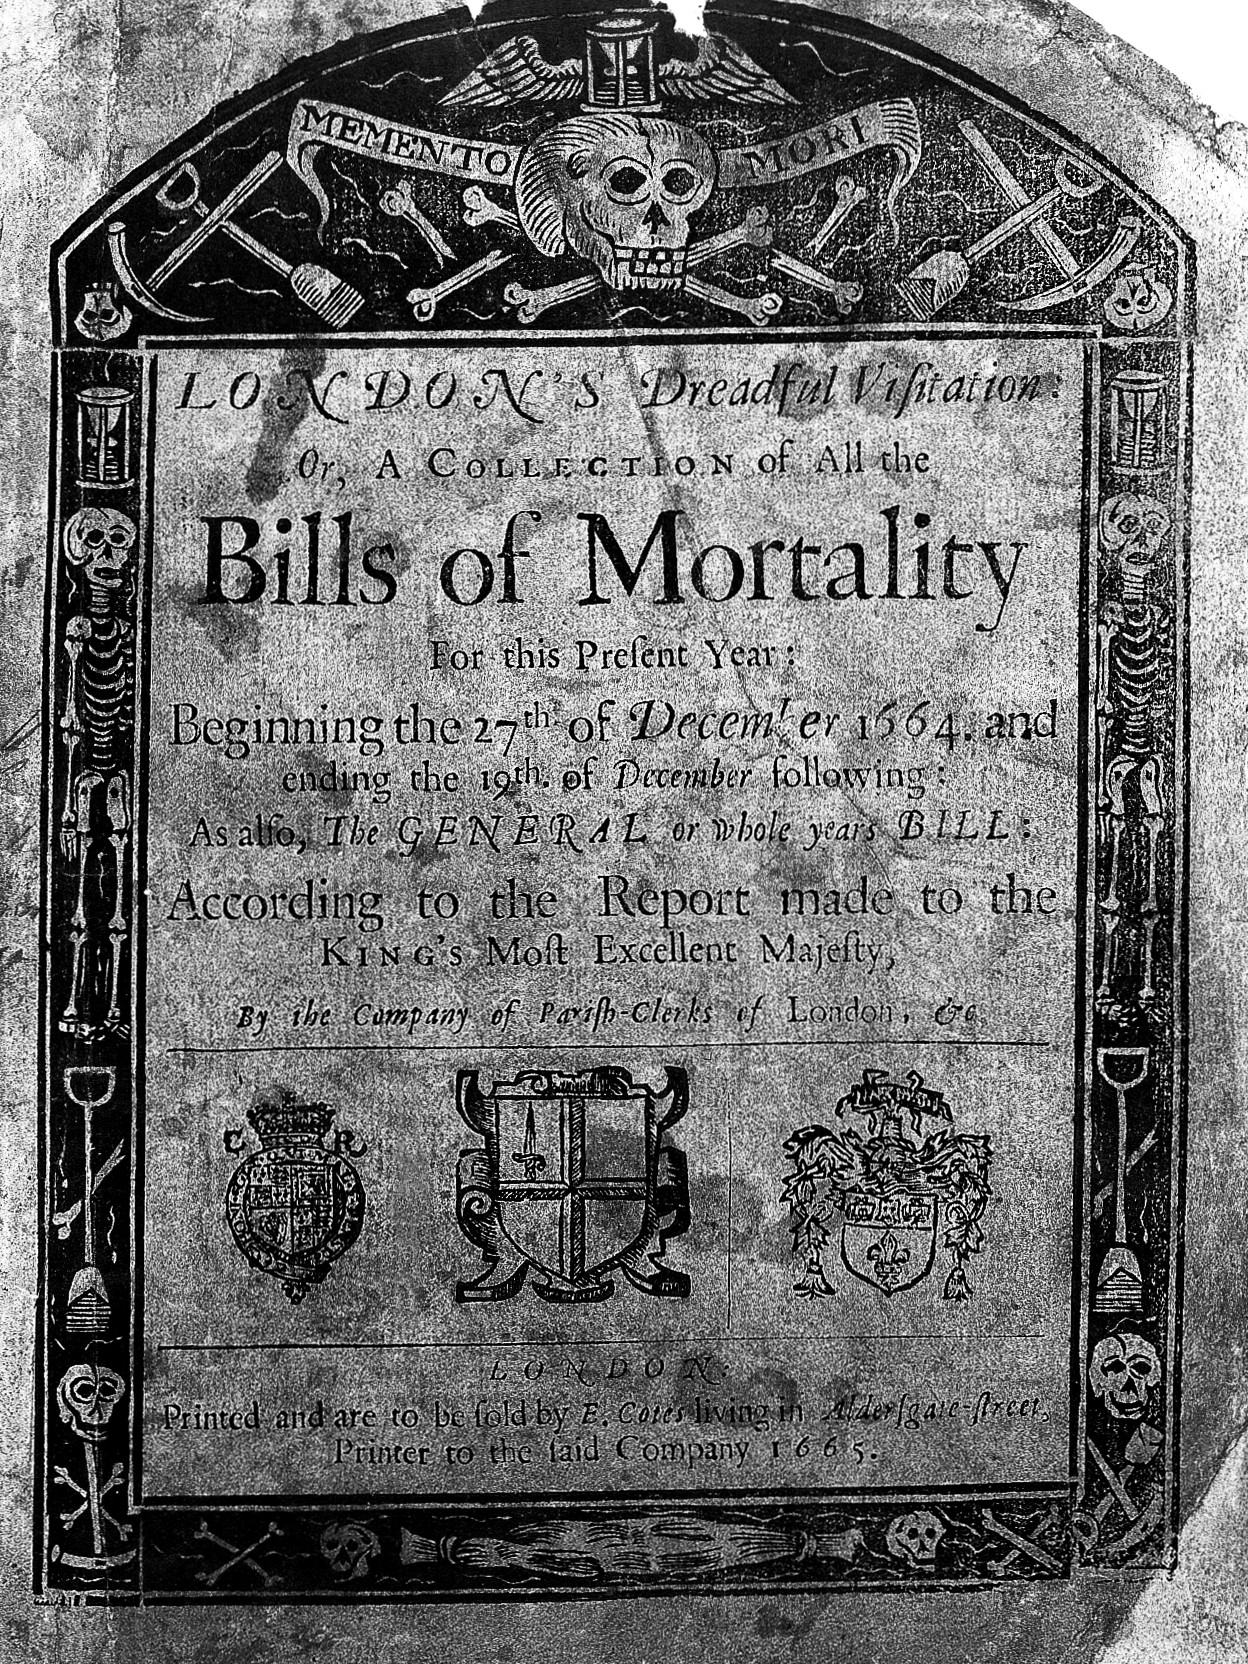
\includegraphics[width=\linewidth]{./figures/bills-of-mortality.jpg}
	\centering
	\caption{London's Bills of Mortality, 1665 (\href{https://commons.wikimedia.org/w/index.php?curid=36040989}{Wellcome Images}).}
	\label{fig:billsofmortality}
\end{marginfigure}

The reductionist scientific method was formalised and scientific institutions were established to embed this radical problem solving approach. Problem-solving was beginning to be predicated upon the 'taking apart' the object of study into its most fundamental parts. Knowledge was gained of each of the parts, which were 'reassembled' to gain knowledge of the 'whole'.

Similarly, scientifically based analyses looked at a problem, for example causes of death in London, and began to identify: how many deaths from each distinguishable cause; the age of the people who died; where they lived; their occupation, etc. Creating knowledge about deaths in the London population began by looking at each part of the problem and then compiling information to get a picture of what was happening.

\subsubsection*{Infectious disease surveillance}

Epidemiology, the science of public health, began to take form mid-nineteenth century, and with it infectious disease surveillance emerged to create the form and function of a first semblance of public health intelligence. Together they began to deliver knowledge of the natural history of disease, its etiology, and occurance, along with information on its incidence and prevalence in the community. Public health practice, as we know it today, began. Happy days!

Notifiable diseases and international standards of reporting have been happening for almost a hundred years. However, the real methodological home of public health intelligence can be found in early efforts to intervene in outbreaks of disease. One example of an early analytical approach to epidemiology and public health can be traced back to at least 1854 and John Snow's map of cholera in London (Figure~\ref{fig:johnsnow}). Thus began the tradition of investigating and reporting on infectious diseases outbreaks, which has contributed to the body of knowledge and practice that is undertaken by all developed nations and under the general rubric of 'public health intelligence' today. More importantly perhaps, the conceptual emergence of 'information for action'.

\begin{marginfigure}%
	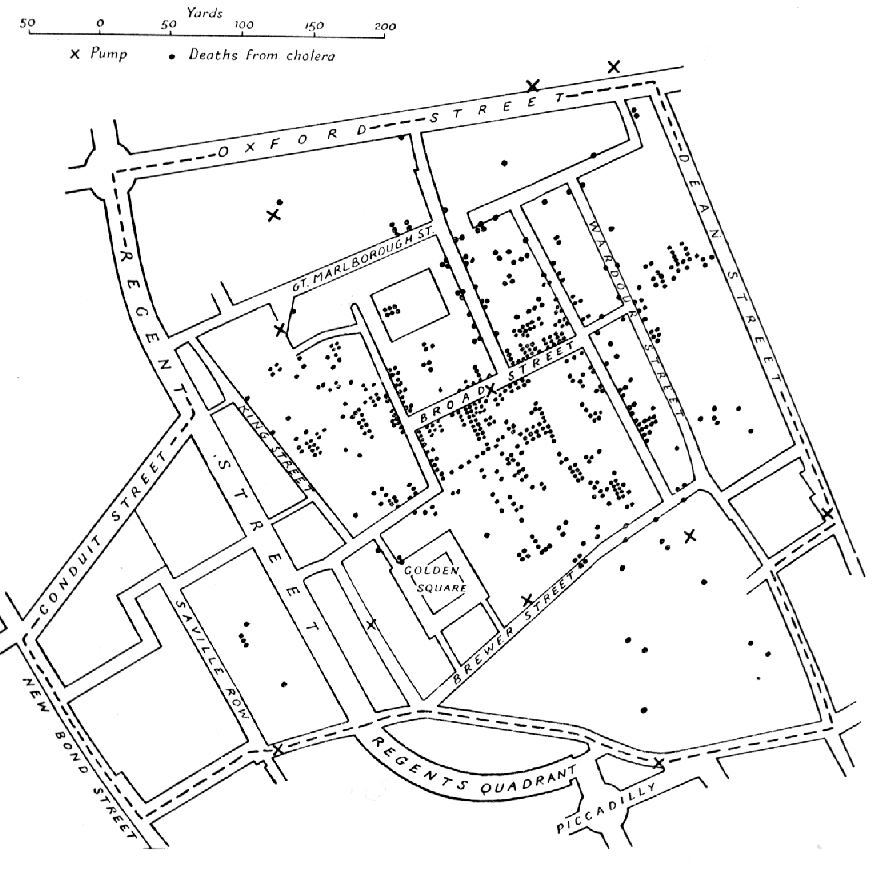
\includegraphics[width=\linewidth]{./figures/Snow-cholera-map.jpg}
	\centering
	%\bigskip
	\caption{John Snow's 1854 cholera map of London denotes the location of deaths and is a very early example of analytical thinking in health intelligence (\href{https://commons.wikimedia.org/w/index.php?curid=403247}{Wikimedia Commons}).}
	\label{fig:johnsnow}
\end{marginfigure}

\subsection{Chronic Disease and the beginning of the Information Age}
The beginning of the information age coincided with the epidemiological transition from infectious to chronic disease in most developed nations.

Public Health Intelligence (mid-20C) -- transition to chronic disease and digital data

The major developments over the last few decades have included moving disease analysis, storage and reporting from paper-based to digital systems. In my experience, a considerable portion of the public health intelligence resource has traditionally been expended on data collection and cleaning processes, not on analysis, let along insight development. Until the recent adoption of a data analytics posture, the tools of the trade had, for a long time, primarily been spreadsheets and relational databases.

\subsection*{Business intelligence and analytics}
Business Intelligence was the private sector's answer to public health intelligence, and with it began the move towards 'analystics' and away from bespoke 'analysis'.

Business Intelligence and Analytics (mid-20C) -- analytics and data warehouses


\subsection*{Data Science} 
Data Science marks the height of the analysis paradigm and so to the beginning of its decline, perhaps. We seem to have come full circle 

Data Science (early-21C) -- beginning of the end for the 'analysis paradigm'



The move to data analytics and adoption of data science methods....

Why?

\section*{Public health intelligence is falling short}
% Why is it falling short? This section title is NOT informative and all 
% sections in ToC need to be informative. I agree it is falling short, but
% why. What case is made below? Need to have a case to be made.
% Off the top of my head:
% 1. We can't see what difference we are making
% 2. PHI currently supports silo'd thinking
% 3. Although we can assess what is happening (events) and anticipate 
%    what is coming next (pattersns), we are unable to adequately analyse
%    the structure of a problem let alone the thinking that underlays that
%    ...

What is the purpose of public health intelligence? I think that most of my colleagues would phrase the response to this question something along the lines of: "The purpose of public health \emph{intelligence} is to deliver high quality \emph{information} in a timely manner to our clients to enable the development of \emph{insights} that facilitate \emph{evidence-based decision-making} that is ultimately successful." There is a bit to unpack here:

\begin{description}
	\item[Intelligence:] A product or activity/function that delivers contextualised information in response to a challenge or question
	\item[Information:] Data with sufficient structure to enable its use in getting 'business' (aka public health interventions) done
	\item[Insights:] An interpretation of information leading to an increase in understanding
	\item[Evidence-based decision-making:] Public health practice is predicated upon the belief that this is what we do, even when sometimes this is questionable
\end{description}

Earlier in the history of public health, prior to the development of an explicit 'intelligence function', disease surveillance teams termed what they did as providing 'information for action'. Despite the broader range of foci across current intelligence functions, this ambitious purpose could be reinterpreted as "intelligence for action". However, public health intelligence appears to be focussed on a much less ambitious goal than earlier infectious disease surveillance efforts had in mind, i.e. 'information for action'(Figure~\ref{fig:IntelLM}).

\begin{figure}
	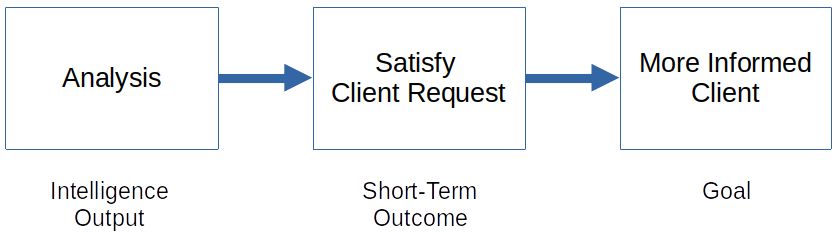
\includegraphics{./figures/Current Intel Logic Model.png}
	\caption[Current PHI Theory-of-Change][6pt]{A simple theory-of-change captures the essence of much of current public health intelligence practice: Do the analysis to satisfy client requests with a view to having a more informed client at the end of the process.}
	\label{fig:IntelLM}
\end{figure}

Indeed, I believe that public health intelligence needs to readopt 'action' as a goal (Figure~\ref{fig:toc}). There may be a couple reasons why we currently don't have the same focus on 'action' that we used to, but they come down to the complexity of communities in which public health is trying to take action. It's not just about 'removing the pump handle'. Chronic disease interventions may require years to demonstrate a result. The result, if there is one, may be masked by other noise within the system and be hard to attribute to the intervention(s).

However, I think that there is also another factor at play, one that we don't discuss very often -- the very nature of public health organisations. Compared with early efforts that were almost entirely focussed on infectious disease interventions, we now have a large number of areas that we try to influence. Therefore, we attempt to 'divide and conquer problems. We create silos, even silos within silo of efforts and domain knowledge. Public health intelligence is a silo. Those who do analysis do not, as a rule, also build and deliver public health interventions. Perhaps the most defining characteristic of public health intelligence is that analysts answer 'client' questions -- that is the new goal.

Public health intelligence analysts are specialists. Epidemiologists also specialise in particular diseases or transmission modes or populations at risk, in ways similar to the specialisation of the medical profession. Analyst participation in public health engagement, planning and action cycle is generally limited to three stages of client request clarification, data processing and analysis  (Figure~\ref{fig:AnalystCycle}).

\begin{figure}[t]
	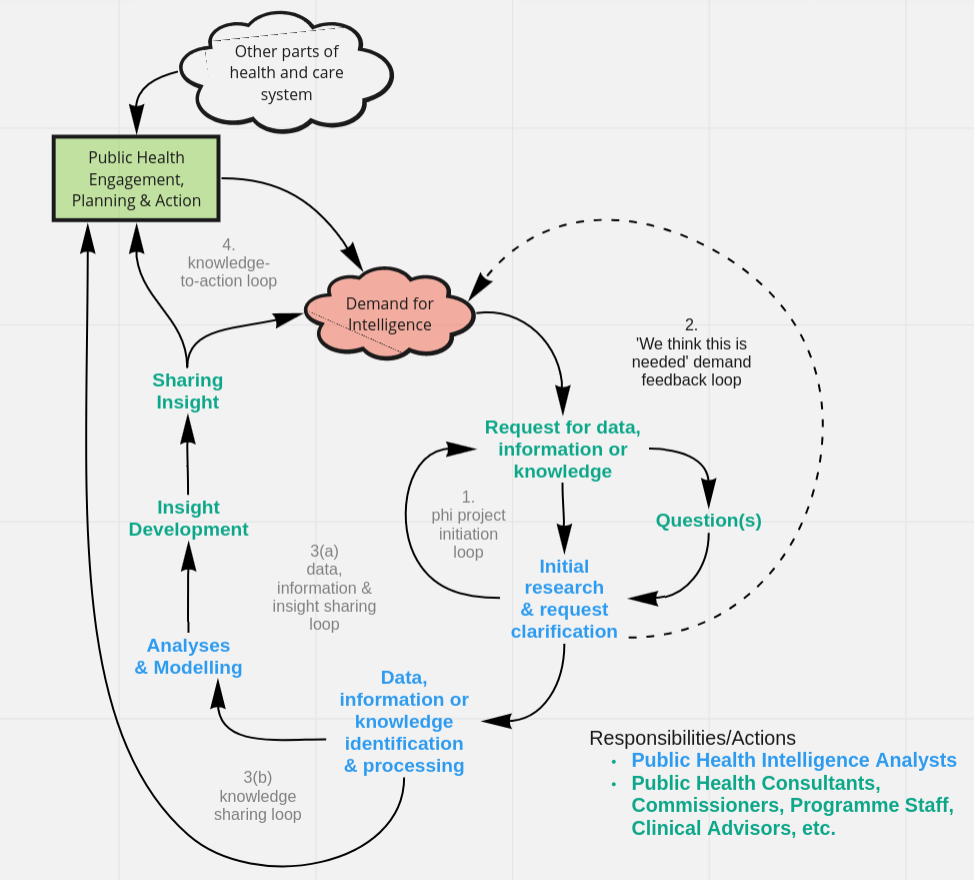
\includegraphics{./figures/PHI Analyst Cycle Draft.png}
	\caption[Current PHI Analyst Cycle][6pt]{DRAFT. Demand for public health intelligence creates a number of feedback loops defining relationships with their public health 'clients'.}
	\label{fig:AnalystCycle}
\end{figure}

Specialisation can be very useful for increasing the efficiency of processes, particularly where advanced analytical skill sets are limited and therefore need to be used to best effect. The problem underlying the request for intelligence is most often quite opaque to the analysts. This is true for a number of reasons that include time pressures, lack of analyst health domain knowledge, the inaccessibility of decision-making forums. It doesn't really matter why we can't see and/or understand 'a client' problem, but the end results is we usually have a fairly incomplete picture of the intelligence need, and means that we can easily be working on the wrong problem.

\begin{marginfigure}%
	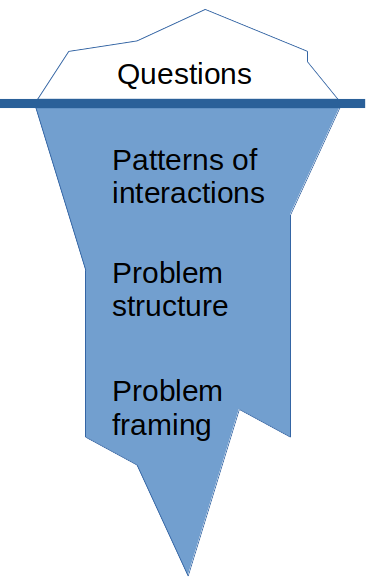
\includegraphics[width=\linewidth]{./figures/PHI Iceberg.png}
	\centering
	%\bigskip
	\caption{Edward Hall's Iceberg model is used here in an attempt to better understand the things we can't easily see about the public health intelligence process.}
	\label{fig:iceberg}
\end{marginfigure}

\subsection{Client questions and problems}
Clients ask analysts questions and analysts try and answer those questions, but if all an analyst can see is the question, they do not have a big enough picture to ensure that they are answering the right questions. Questions are therefore what the analyst sees, like an iceberg (Figure~\ref{fig:iceberg}). It is what remains out of sight, ie. below water that remains dangerous, and while an analyst can infer much about the problem through repeated engagement with clients over time, the analyst rarely develops sufficient knowledge about the structure and framing of the problem. Therefore, the extent of the danger of the hidden iceberg and of not answering the right question remains.

Ultimately, only decision-making that is underpinned by science is deemed acceptable in most modern health and care systems. Science, aka scientific reductionism, is the theoretical basis for the analysis process. Consequently, the analysis paradigm has been the only approach available to most analysts.

Indeed, most of us are Analytical Thinkers. This paradigm is so engrained that when we consider the meaning of the term 'thinking', we are actually describing 'analytical thinking'. That shouldn't be surprising as this paradigm has been at least 400 years in the making, deriving from  the reductionist scientific approach to problem solving and knowledge acquisition. The science under-pinning most of public health is epidemiology, and epidemiology is a reductionist scientific discipline.

\subsection{Ackoff's description of analytical thinking}
'Analytical thinking' is a term created by the organisational theorist, Russel Ackoff, to describe the paradigm by which we attempt to solve problems. We respond to problems or challenges identified by our organisation using Analytical Thinking in three basic steps (Table~\ref{tab:analysisthinking}).

\begin{table}[h]
	\begin{center}
		\footnotesize%
		\begin{tabular}{p{4cm} p{6cm}}
			\toprule
			Process & Example  \\
			\midrule
			Step 1: Disaggregate problem & CVD deaths into deaths by sex, age, co-morbidities, deprivation\\
			Step 2: Examine each part & Statistically describe and analyse of patterns\\
			Step 3: Reassemble for an understanding of the whole & Model the relationships between risks and outcomes\\
			\bottomrule
		\end{tabular}
	\end{center}
	\caption{Russell Ackoff's three step process defining 'Analysis Thinking'.}
	\label{tab:analysisthinking}
\end{table}

This process is the dominant paradigm in health intelligence, and it has served us well for many decades\cite[-1\baselineskip]{RegmiandGee2016}. However, we also know that working with clients to identify the ‘intelligence challenge’ and any underlying questions is often a long iterative process. It is often unsatisfying because the ‘client’ often does not want to invest a lot of their time – ‘they just want the data’ (actually they want information, but let's not quibble).

However, our ‘single minded approach’ to health intelligence is largely responsible for the difficulties we experience in effectively engaging with clients – there appears to be only one way to support decision-making and that’s through Analytical Thinking (Figure~\ref{fig:at1}).

\begin{figure}
	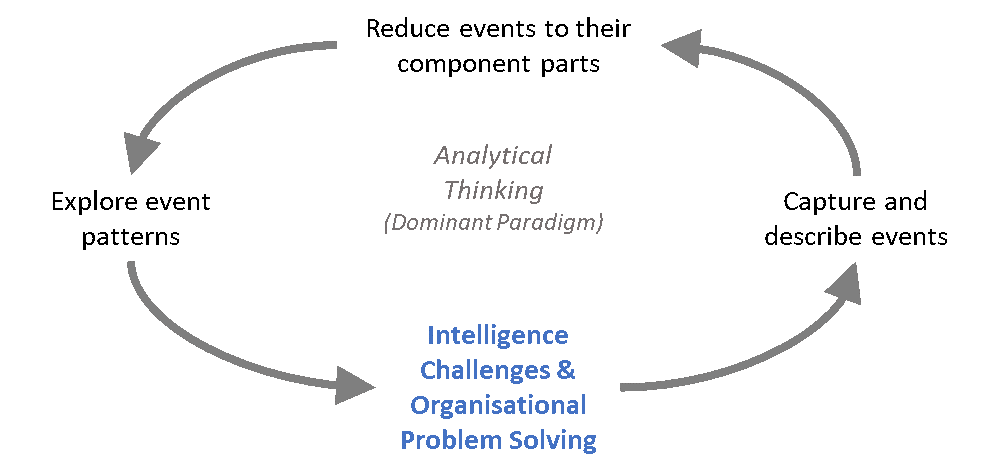
\includegraphics{./figures/analytical thinking feedback loop.png}
	\caption[Analytical Thinking is powerful][6pt]{Analytical thinking, while increasingly powerful through the adoption of data science methods, nonetheless provides a single approach to organisational problem-solving and the support of decision-making.}
	\label{fig:at1}
\end{figure}

The domination of Analytical Thinking over any other type of approach to problem-solving didn’t happen by accident, it is a product of the very successful reductionist scientific approach (Figure~\ref{fig:at2}). The problem we now have, and most analysts sense this, is that what worked well for understanding diseases, viruses and the like, doesn’t quite deliver the same understanding when applied to health systems where human decision-making, organisational culture and complex inter-organisational structures create complexity and dynamics/behaviours. This is our ‘problem-solving’ space.


\begin{figure}
	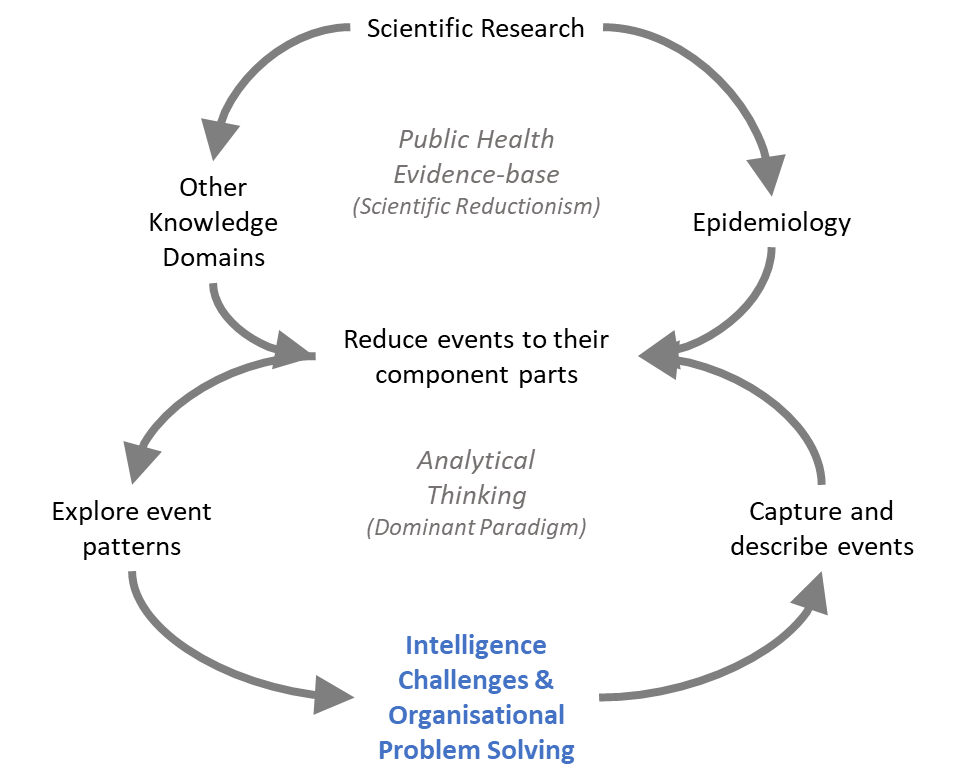
\includegraphics{./figures/analytical thinking reductionist science.png}
	\caption[Analytical Thinking is reductionist science[6pt]{Analytical thinking is driven by the same reductionist processes that are at the heart of most scientific research. This approach to problem-solving has been hugely successful delivering the ‘public health evidence-base’, but it is limited in what it can explain about the functioning of systems that include human behaviour, e.g. health systems.}
	\label{fig:at2}
\end{figure}

\subsection{Two Key Public Health Intelligence Challenges}

To be sure -- public health intelligence has many challenges, but I think two challenges are fundamental as they speak to the effectiveness of this critical function.

\begin{enumerate}
	\item Operational Challenge: Every public health intelligence group struggles with 'client engagement' that is centred around identifying and articulating what it is that the client really needs.
	\item Strategic Challenge: The bigger picture problem is that in most organisations, the intelligence function is limited to gathering, managing and analysing data. I think that this is a very short sighted view of the 'intelligence function' and what we really ought to be doing to be focussing on is working with colleagues to solve organisational problems, not fling data all about , which is mostly counter productive.
\end{enumerate}


\section*{Why preventing ill health seems beyond our ken}

Analytical thinking has had its day, it transitioned us away from the 'dark age' into a period of 'enlightenment'. Problem solving from the Renaissance onward has be dominated by reductionist scientific thought that has delivered massive advances in knowledge and technology. It created the 'machine age' and later the 'information age'. Knowledge continues to rapidly grow today, and yet there are more and more global and local problems that we can't solve: Climate heating, environmental degradation, loss of biodiversity, war, poverty, inequality, population health, healthcare affordability. The list is seemingly endless.

It could be argued of course that we choose not to solve many of these problems, not that we can't solve these problems. There is certainly a whiff of that in our political, social and cultural lives. Nonetheless, I think that most people would identify these as problems to be solved. Many writers have suggested that we are currently transitioning from the 'information age' into the 'systems age', and that our approach to thinking and problem solving needs to follow, if we are to continue solving real-world problems.

\begin{itemize}
	\item when did things get too complicated?
	\item R Ackoff quote about a scientific conference in late 1800s where they thought they would have a complete explanation of everything
\end{itemize}

Operationally, public health intelligence needs to reassess it's engagement will clients. I think we need to change from an 'intelligence as service' posture to an 'intelligence as a consultancy' posture where we (a) acknowledge that our public health colleagues are just as important to the intelligence function as are the analysts, in fact they are an integral component of the intelligence function (we just pretend that they aren't); and (b) we need to think differently in a number of ways, but most importantly we need re-engage the public health workforce with 'systems thinking' and we need to co-design the intelligence delivery.

Strategically, public health intelligence should refocus on supporting organisational problem solving. Population health intelligence does not in and of itself improve the health of the population. Surely, this is self-evident to most people? However, just to reinforce the above quote and differentiate population health intelligence from activities that have the potential to change the health of the population: 

\begin{adjustwidth}{3em}{0em}
	\begin{description}
		\item[public health interventions] can improve population health;
		\item[sound public policy] can improve population health;
		\item[reducing poverty] can improve population health;
		\item[decreasing inequality] can improve population health.
	\end{description}
\end{adjustwidth}

If public health analysts do not do these things, how then can we use population health intelligence to improve the health of our populations? For a start, we need to stop working in silos. An oft repeated mantra in some quarters, but how do we actually achieve it? The second change we need to make and this maybe seen as heresy in some quarters, but we need to stop focusing on 'intelligence' and start focusing on 'problem-solving'.

Inscribed on Marx's tomb is the following very apt challenge to public health analysts (except he was speaking of \emph{philosophers}), and perhaps, we should incorporate this challenge into our building systems-based public health practice, as

\quotation{%
	\centering
	The \emph{analysts} have only interpreted the world, in various ways.\linebreak The point, however, is to change it.\footnote{\href{https://en.wikipedia.org/wiki/Tomb_of_Karl_Marx}{Wikipedia:} Karl Marx's Tomb}
}

% Left over from a former section 3.2 in next Chapter -- wasn't a good fit 
% after the last rewrite

Let me start with a different question, since most of us are first and foremost (if not solely) analysis thinkers -- what makes 'good analysis practice'? Here are some thoughts
\begin{itemize}
	\item You know how to formulate problems in a manner that allows to you analyze them
	\item You are able, from knowledge of the problem (business need) and of analysis methodology, to match problems to method
	\item You are also able to adjust methodology based on the nature of the data you have available and appreciate the limitations of methods and data
	
	\item You are able to process data into suitable formats for analysis
	\item If you are suitably experienced you are able to interpret the results of analyses that you or other perform
	\item You are able to apply these insights and/or communicate them to others such that the analysis is useful to the organisation
\end{itemize}




\chapter{Complexity Impaired Decision-Making \& Leadership}
\openepigraph{Complexity is the enemy of execution}{Tony Robbins}

\marginnote{
	\newthought{Key Message:} Decision-making and leadership in the public sector are less effective than they otherwise could be in a world that was less complex. The loss of effectiveness to increasing complexity isn't always reflected in a loss of efficiency, we can still be very productive working on the wrong problems.
}



\chapter{Rethinking Our Approach}
\openepigraph{We cannot solve our problems with the same level of thinking that created them.}{Albert Einstein}

\marginnote{
	\newthought{Key Message:} 
}

\newthought{Public health practice} is core business for a relatively small number of people compared with healthcare. However, we have many colleagues outside of public health who are actively engaged with public health practice (health sector colleagues, academics, social care, etc.) or who at least have an identifiable role to play in the delivery of public health outcomes (including environmental practitioners, hospitality workers, those in administrative and management roles, etc.)\footnote{While the 'few of us', in the UK, is probably more than 40,000, we also have more than 14 million colleagues with a direct role to play. That's a lot of us and we work in many organisations, health systems, and sectors! Source: Centre for Workforce Intelligence. July 2015. Understanding the wider public health workforce, GOV.UK.}.

Public health analysts and decision-makers at all levels, I'm writing this for you. If, like me, you feel that something is missing or that you aren't getting the impact from your organisation's intelligence function that you need, then maybe what follows will be food for thought, maybe even useful.

I am speaking directly to my public health colleagues about the public health intelligence function. More broadly, I would expect that this content may also resonate with public service colleagues outside of health because I suspect that they face similar intelligence challenges. If you are a problem-solver, I hope that this book is welcome food for thought and I certainly welcome your thoughts in return\footnote{The best way to reach out to me is through my (\href{https://www.linkedin.com/in/wchrrisskelly}{Linkedin Profile}). I'm interested in any constructive thoughts, feedback or genuine conversations on the topics within\ldots}.

For those colleagues who see public or population health intelligence in a more traditional light, focussing on collecting, processing and analysing of numerical data, then you'll be disappointed with the very shallow to non-existent treatment of those topics in this book. The 'bills of mortality' have been done to death (pun intended). Nonetheless these are still important topics inasmuch as we still seem to get these analyses wrong, and their data science equivalent data analytics wronger (not a word, but this too was intended). However, if you want to understand why we get them wrong and how we can fix them, then please follow along, as we will be exploring this aspect of the 'traditional' population health intelligence process.



\section{How to move your organisation towards a systems-based practice}

\begin{enumerate}
	\item Understand where we are now -- Analysis Paradigm
	\item Develop a cognitive model for systems based practice
	\item Implement systems based public health practice
	\item Create organisational learning to power the transformation
\end{enumerate}

This story has a main four parts. However, the first three parts are set out 'from outside in', and like an onion we have a look at each and peel them away in order to appreciate the next layer (Figure~\ref{fig:apptosensemaking}). You may also notice that, at least for analysts, that this is from least familiar to most familiar. However, and perhaps most importantly, we are dealing with biggest picture first in futures thinking---the business needs, which is all too often forgotten in the rush to crank the handle and produce data, analytical thinking, which we'll deal with last.

The first part, futures thinking, is big---hopefully infinite. It relates to our business need, which in population health intelligence is very big indeed. If you work in a hospital your business needs are defined by your patients, staff, healthcare services, legislation, regulation, contractual obligations, infrastructure, health outcomes, etc. The key bits for an analyst to consider:
\begin{itemize}
	\item You should know that the business need associated with every request for intelligence, but if your intelligence process is treated like Mr Ford's first assembly line, you might not. If that's the case, you are missing a big chunk of being able to create intelligence for action. It is 'why' you are trying to answer the question (if are lucky enough to have one of those) in front of you.
	\item Analysts have plenty of skills that can be used to understand and articulate business needs.
	\item Business needs don't stay the same, ever. The world changes.
\end{itemize}

The second part we look at is systems thinking. Systems thinking is big too. Maybe not as big as futures thinking, but systems thinking is focussed on the here-and-now. Systems thinking can certainly be used to understand business needs, but it can also be used to identify and frame the exact questions we should be asking from the intelligence process. I can't be the only analyst to have ever worked with colleagues who didn't seem to have a question and after much iterative effort discovered that:
\begin{itemize}
	\item the question has already been answered
	\item the wrong question is being asked
	\item that there really is no question
\end{itemize}

The third part of this onion is analytical thinking. This comes last, because you already know about this one, or at least you should know about this type of thinking---its what you do every day. It is our dominant problem-solving paradigm, and it used to work really well until, well it stopped providing solutions that stick. We'll have another look at this type of thinking, we'll discuss why it doesn't work particularly well on its own anymore---particularly for decision-makers, who might also not realise that it isn't working particularly well anymore.

The fourth and last part is about how we integrate these three approaches to the provision of intelligence in order to build problem-solving capability within our organisation or health system. It's less about intelligence process and method, and more about organisational development to achieve better population health intelligence.

\marginnote{
	\newthought{Key Message:} Public health attempts to create change within communities to protect and improve the health of those populations. In this, it is guided by public health intelligence activities that are entirely focussed on turning data into useful information that can guide these interventions. These are evidenced largely from epidemiology, a reductionist science. Consequently, if your problem cannot be understood and solved by breaking it into smaller parts, understanding each part on its own, then you have a major limitation.}

I've spent many years working in public health intelligence. Its been a passionate intellectual pursuit since at least the mid-1990, a period during which I was peripherally involved in the response to dengue outbreaks in North Queensland, Australia. So when I say that the 'analysis paradigm' -- the fundamental way we think, act and learn about things like disease outbreaks -- constrains past public health practice. I expect to be looked upon as a heretic. I'm as invested in this paradigm as are any of my public health colleagues.

I chose the word 'constrain' quite carefully though. Heretical is one thing, being burnt at the stake is quite another! Seriously though, I don't think for one moment that our current practice of public health hasn't benefited our communities. Of course it has and it will continue to benefit society at large; it's just that it's effectiveness is declining as complexity increases. We are still using a 19th century approach to problem solving.

I'm devastated for the same reason many of my intelligence colleagues are -- we can't see that we are having an impact any more. However, I'm also amazed, because unlike many of my colleagues I can now clearly see why this is the case.

The challenge in being able to see the problem is not a simple one, it involves: (1) evaluating whether we are indeed having an impact and to do this (2) what would this 'positive impact' look like? I have only ever tried to evaluate this once, a study of the key workforce issues for public health intelligence analysts across a region of England (Appendix~\ref{ch:case_study_3}). 

We found that our inability to see whether we are 'making a difference' could be a prime driver of job dissatisfaction. If I hadn't also been looking deeply into systems thinking, I might have left it at that. Can't see impact. Unhappy. Do something else outside public health. I know that I'm not the only person in public health intelligence who feels like this sometimes. It is a growing feeling amongst many colleagues and we should be worried about it.

However, what we see are three feed back loops (Figure~\ref{fig:SWAnalysts}). Two of these feedbacks, organisational learning and intelligence delivery appear to be reinforcing loops, which means that when things are getting better they tend to keep improving and when things are getting worse, they keep getting heading in that direction. Job satisfaction is definitely declining amongst the analysts we interviewed.

\begin{figure*}
	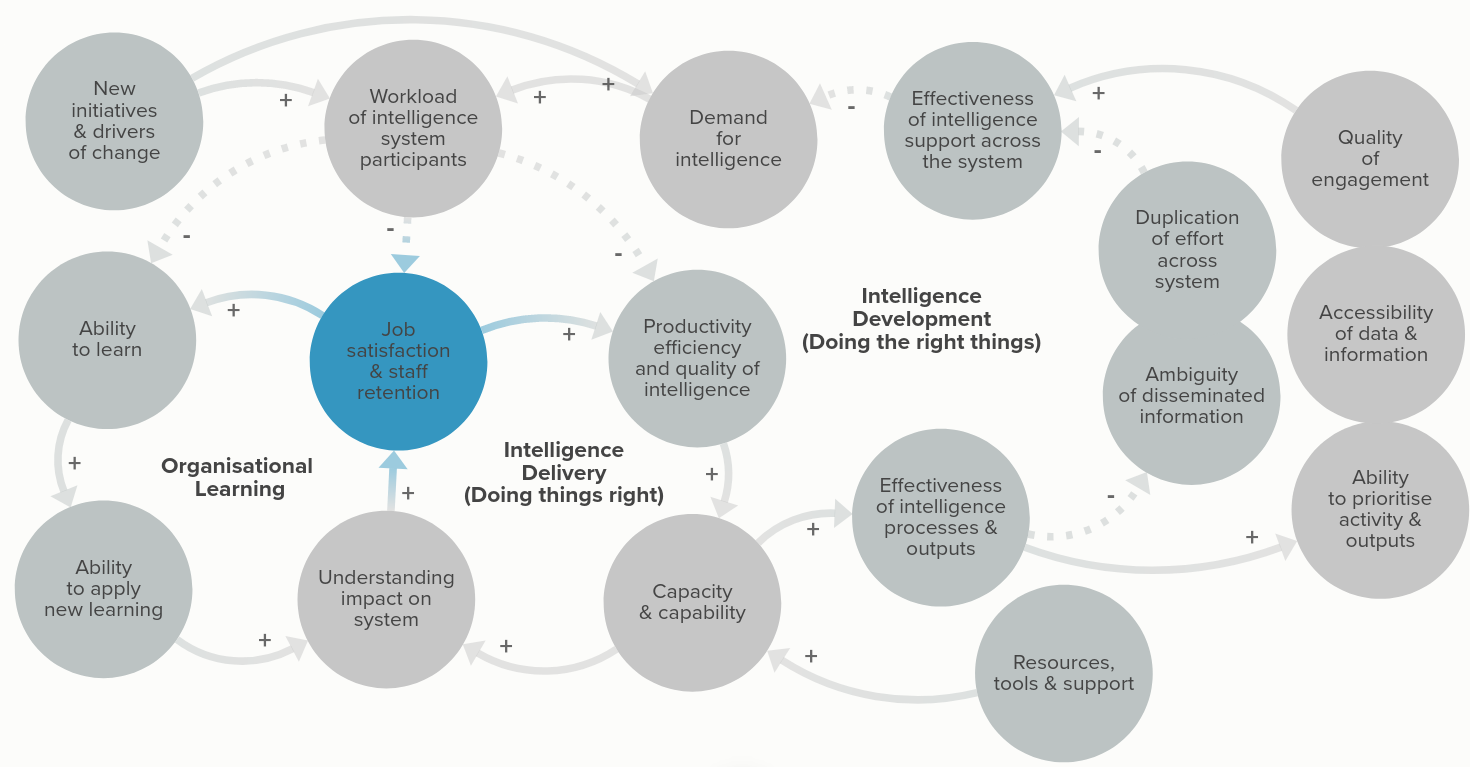
\includegraphics{./figures/SWAnalystChallenge.png}
	\caption[Public health intelligence effectiveness][6pt]{A causal loop diagram illustrates three feedback loops in regional intelligence that are likely reducing the effectiveness of public health intelligence.}
	\label{fig:SWAnalysts}
\end{figure*}

A third feedback loop, intelligence development, is much more messy, but it is of most interest to me. Its about effectiveness of public health intelligence. Does it make a difference -- so it speaks to the central question here! The feedback loop suggests that unless we have an increasingly effective system of public health intelligence demand for intelligence will continue to grow (because it isn't be satisfied), workloads will continue to grow (beyond what is manageable), and analyst job satisfaction will continue to grow with all the flow-on effects illustrated.

What I can now see is that the complexity of society in general would never all us a clear view of our impact, and this is true for public health as a whole. Population health and its improvement is never going to be easy to see or attribute blame or credit to a single effort. One only has to consider the case for smoking and cancer and heart disease. Slam dunk, right? Consider how many years public health has been on the case, how many interventions have been required (taxation, regulation, legislation, education, treatment, etc.). We've thrown everything at this and we were rewarded with initial years of decrease followed by a levelling of the trends and now projected increases. What is going on?

Complexity. Complexity is what's going on. Our view of population health has been constrained by complexity. Our practice of public health has similarly been constrained by complexity. Consequently, public health practice is primarily reactive in nature with at best some short-term ability to anticipate what is coming next. Emphasis on 'short-term'. At the heart of our inability to 'see' is the current practice of public health intelligence, which despite huge advances in analytical methods, is only incrementally improving practice.

This chapter sets out past and current public health practices as underpinned by public health intelligence activity. The current contraints in practice cannot be solved by incremental improvement, and require a new approach. What follows is the story of how we got into this situation and what it means.


\section{The journey out of the analysis thinking}

Absolutely everything I looked at over the next 20 years seemed to be complex, and almost nothing in my university education equipped me to apply science and analytical skills to support the resolution of problematic situations in the real world... (new para or subsection) earth observation science... (new para or subsection) climate impacts science... (new para or subsection) academia heaven and hell... (new para or subsection) Dengue!


%
% Part II: Embracing Systems Thinking
\part[Embracing Systems Thinking]{Embracing System Thinking in the Public Sector}

\chapter{The Transformative Power of Systems Thinking in Public Health}

\chapter{Tools and Techniques for Systems Thinking in Public Health}

\chapter{Applying Systems Approaches to Health Promotion and Illness Prevention}

\chapter{Fostering a Systems Thinking Culture in Health Organizations}

\chapter{Integrating Systems Thinking Across Health Sectors}




%
% Part III: Building a Critical Systems Practice
\part[Building A Critical Systems Practice]{Building a Critical Systems Practice to Ensure Health System Resilience}

\chapter{introduction to critical systems thinking in public health}
\chapter{methodolgical pluralism in public sector health leadership}
\chapter{participatory and emancipatory approaches in population health}
\chapter{implementing critical systems practice in public health policy}
\chapter{evaluating complex public health interventions through a CST Lens}
\chapter{cultivating adaptive public sector leadership with CST}


% Following command adds "Appendices" to the ToC
% without numbering it
%\addcontentsline{toc}{part}{Case Study Appendices}
\part{Case Study Appendix}
%\appendix
\chapter{Case Study 1: Population Health Impacts Of Climate Heating}
\openepigraph{%
	A ruined planet cannot sustain human lives in good health. A healthy planet and healthy people are two sides of the same coin.
}{Dr. Margaret Chan, Executive Director, WHO}

\marginnote{
	\newthought{Key Message:} The impact of climate heating on local populations is a truly wicked problem that public health practitioners spend very little time thinking about. It's too hard. It isn't a health system priority; it is tomorrow's problem. We need to make it easier to understand and incorporate into all local population planning. Systems thinking might provides some useful tools.
}

\section{Complexity and Public Engagement}
The aim of this document is to bring together all threads of this project that set out to explore how public health could develop policy in the area of potential health impacts from climate change on the older population of West Dorset. It became obvious quite early in the project that this was not going to be an easy task. The difficulty arises firstly in developing a meaningful engagement on the topic. Getting attention for a problem that is in the future, and not thought to be more significant in impact than many current population health issues was always going to be a challenge.

We have approached this challenge by adopting a `systems thinking' approach to our engagement with policy makers and `futures studies' approach in our engagement with the community more widely. In truth, these approaches are complementary and underpin both engagement processes.

\begin{description}
	\item[Systems Thinking]An approach to developing deeper understanding of complexity by examining problems and challenges within the context of the `system' in which they exist.
	\item[Futures Studies] An approach to the development of strategy that seeks to understand an issue or challenge in the context of a more comprehensive picture of a future state. Incorporates a fundamental belief that at any point in time there are many possible futures -- strategically one should work towards a preferred future.
\end{description}

\subsection{Change of Project Emphasis}
The project that began as a climate change impacts on the health of older persons in West Dorset, ended as a project entitled, \emph{Complex Challenges \& Public Engagement}, reflecting the broader issues we encountered during the running of this project.

Our change in emphasis was not an abandonment of the initial research focus that sought to develop a better understanding of what impacts older people in West Dorset would face in thirty years. Indeed, it was our desire to make a meaningful contribution in this area that we realised that our initially more traditional research approach had two shortcomings:
\begin{enumerate}
	\item Scientific uncertainties regarding the estimated outcomes 30 years in the future are such that we would not succeed in delivering new information, but rather our approach would include the same lists of possible outcomes and generalised mortality outcomes; and
	\item Consequently, the initial difficulties we experienced in engaging stakeholders would be compounded, because we had nothing particularly compelling to engage with.
\end{enumerate}

\subsection{Project Outputs}
Thus far this project has presented a number of workshops, a conference poster and delivered a systems model and story, various futuring deliverables including a Futures Story and this report.

It is anticipated that these materials will be used further in 2016 to continue exploring the public health challenge faced by climate change in Dorset and we will also seek to publish some of this work.

Furthermore, a longer term outcome will require a longer effort as we attempt to apply the methods explored here to other public health challenges over the coming years.

\subsection{Project Outcomes}

Ultimately, Public Health Dorset role is to protect and improve the health of its population -- we hope that methods adopted during this project will contribute towards the success of that role. However, a more immediate outcome has been the exposure of many staff to systems thinking and futuring methods, which now extends their potential reach in developing shared understanding of particularly complex public health challenges.

\subsection{Report Organisation}

Part I of this report focusses on the `systems thinking', `systems modelling' and `systems story telling' methods that were used in an effort to develop a shared understanding of this public health challenge.

Part II reports on the use of future methods: `horizon scanning', `scenario building' and `futures story telling'.

Part III of this report serves as a repository for presentations and stakeholders events, recording the evolution of the group's thinking over the two year life of the project.

\subsection{Public Health and Systems Thinking}
Systems Thinking as an approach to problem solving appears to have evolved from a sub-discipline of Engineering, Systems Dynamics, and the work of Jay Forrester.\cite{WikipediaJWF} However, it has been used more broadly to explore problems in natural systems, business and organised problem solving more generally.\cite{Ford2010, Senge2006, MaaniCavana2007}

The articulation of systems thinking as a tool in the practice of public health has only occurred relatively recently in explicit reference to `systems', ``The whole concept of public health is founded on the insight that health and illness have causes or conditions that go beyond the biology and behaviour of the individual human being''.\cite{Midgley2006} While, this has always been implicitly understood in modern public health, 

\begin{quotation}
\ldots there is no single operational method for identifying and interpreting these relationships, there is, in fact, a common conceptual orientation recognizable as a systems approach: it is a paradigm or perspective that considers connections among different components, plans for the implications of their interaction, and requires transdisciplinary thinking as well as active engagement of those who have a stake in the outcome to govern the course of change.\cite{Leischow2006}
\end{quotation}

It is clear that a systems approach is intuitively sensible and that the methods available have matured to make its adoption in public health practice both timely and practicable.\cite{Trochim2006, Homer2006} Nonetheless, we still to this day have relatively few examples of its use at the `coal face', and the authors of these works are academics and management consultants.

More recent work looking at the use of a systems approach in disentangling health disparities and health system policy are aimed at experts in their respective fields and not at developing a shared understanding of the public health challenge to public health practitioners.\cite{Roux2011} Indeed, one could question the degree to which these authors truly understand sytems thinking and the application of causal loop and other methods when talking of `health systems' and making only the most rudimentary attempt to actually visualise and map the system.\cite{BoschCapblanch2012} Nonetheless, the effort to improve the targeting of these methods and make a difference in public health continues,

\begin{quotation}
Recognizing that a problem exists and taking action to solve a problem are two activities that many do well, but there is an in-between step that often receives inadequate attention. The source of all important management blunders can be traced back to a mistake in accurately discerning what is important in a situation and incorrectly formulating a problem to be addressed.\cite{Canyon2013}
\end{quotation}

\section{Health Impacts of Climate Change on an Ageing Population}

With this background of a rather recent and not-so-successful introduction of public heath to systems thinking methods, we have focussed on a systems approach because it seemed the only way to adequately address this problem in a way that would make meaningful communication with all stakeholders possible.

\subsection{The Big Picture}
There is a scientific consensus that anthropogenic climate change is increasing global temperature and that this will continue for at least another century. This will impact human health and well-being because the links to human health and climate are well understood.

\begin{quotation}
The health of human populations is sensitive to shifts in weather patterns and other aspects of climate change (very high
confidence). These effects occur directly, due to changes in temperature and precipitation and occurrence of heat waves, floods, droughts, and fires\ldots Until mid-century climate change will act mainly by exacerbating health problems that already exist (very high confidence)\ldots (p. 713)\cite{IPCC2014}
\end{quotation}

The impact of climate change on older persons will be particularly problematic, because

\begin{quotation}
Older people are also more likely to suffer from health conditions that limit the body's ability to respond to stressors such as heat and air pollution\ldots (p. 718)\sidenote{Citation as above.}
\end{quotation}

The range of potential health impacts identified is lengthy and includes:\cite{Portier2010}
\begin{itemize}
\item Asthma, Respiratory Allergies, and Airway Diseases
\item Cancer
\item Cardiovascular Disease and Stroke
\item Foodborne Diseases and Nutrition
\item Heat-Related Morbidity and Mortality
\item Human Developmental Effects
\item Mental Health and Stress-Related Disorders
\item Neurological Diseases and Disorders
\item Vectorborne and Zoonotic Diseases
\item Waterborne Diseases
\item Weather-Related Morbidity and Mortality
\end{itemize}

There have been numerous substantial reviews on the potential health impacts of climate change on the human population and potential mitigation strategies from the WHO\cite{WHO2014a,WHO2014b, WHO2015}, the IPCC\cite{IPCC2014}, the US\cite{Portier2010, Luber2014} and the UK\cite{HPA2012, LancetCom2015}.


The general consensus is that climate change will impact human health in a myriad of ways in the not distant future and that the focus should now turn to mitigation of health impact. There does not, however, appear to be a simple recipe that can be applied and the consequences for much of the developing world will be far more severe than that in the developed world. Nonetheless, scientific evidence suggests that the impacts will be severe and measurable.


\subsection{Temperature Stress Attributable Excess Mortality}
Temperature stress to human physiology, both cold and warm, is relative to whatever is considered to be a 'normal' temperature range. It is important to emphasise that excess mortality related to cold and warm temperature stress is evident at very average temperatures. A recent English study indicates that local temperature stresses occur over very average temperature ranges.\cite{Hajat2014}

In Dorset, UK, temperature stress is estimated to occur when it is either warmer than 17.6 deg C or cooler than 12.1 deg C. The relative risk (RR) of death increases by approximately 2\% for each degree C beyond these thresholds (Figure~\ref{fig:rr}).

As a consequence of Dorset's ageing population, excess winter mortality in the Southwest will continue to be far more of a problem than excess heat related deaths even in a warmer world of 2044. This counter-intuitive finding is entirely driven by the demographic trend of an ageing population.


\begin{figure}[htbp]
\centering
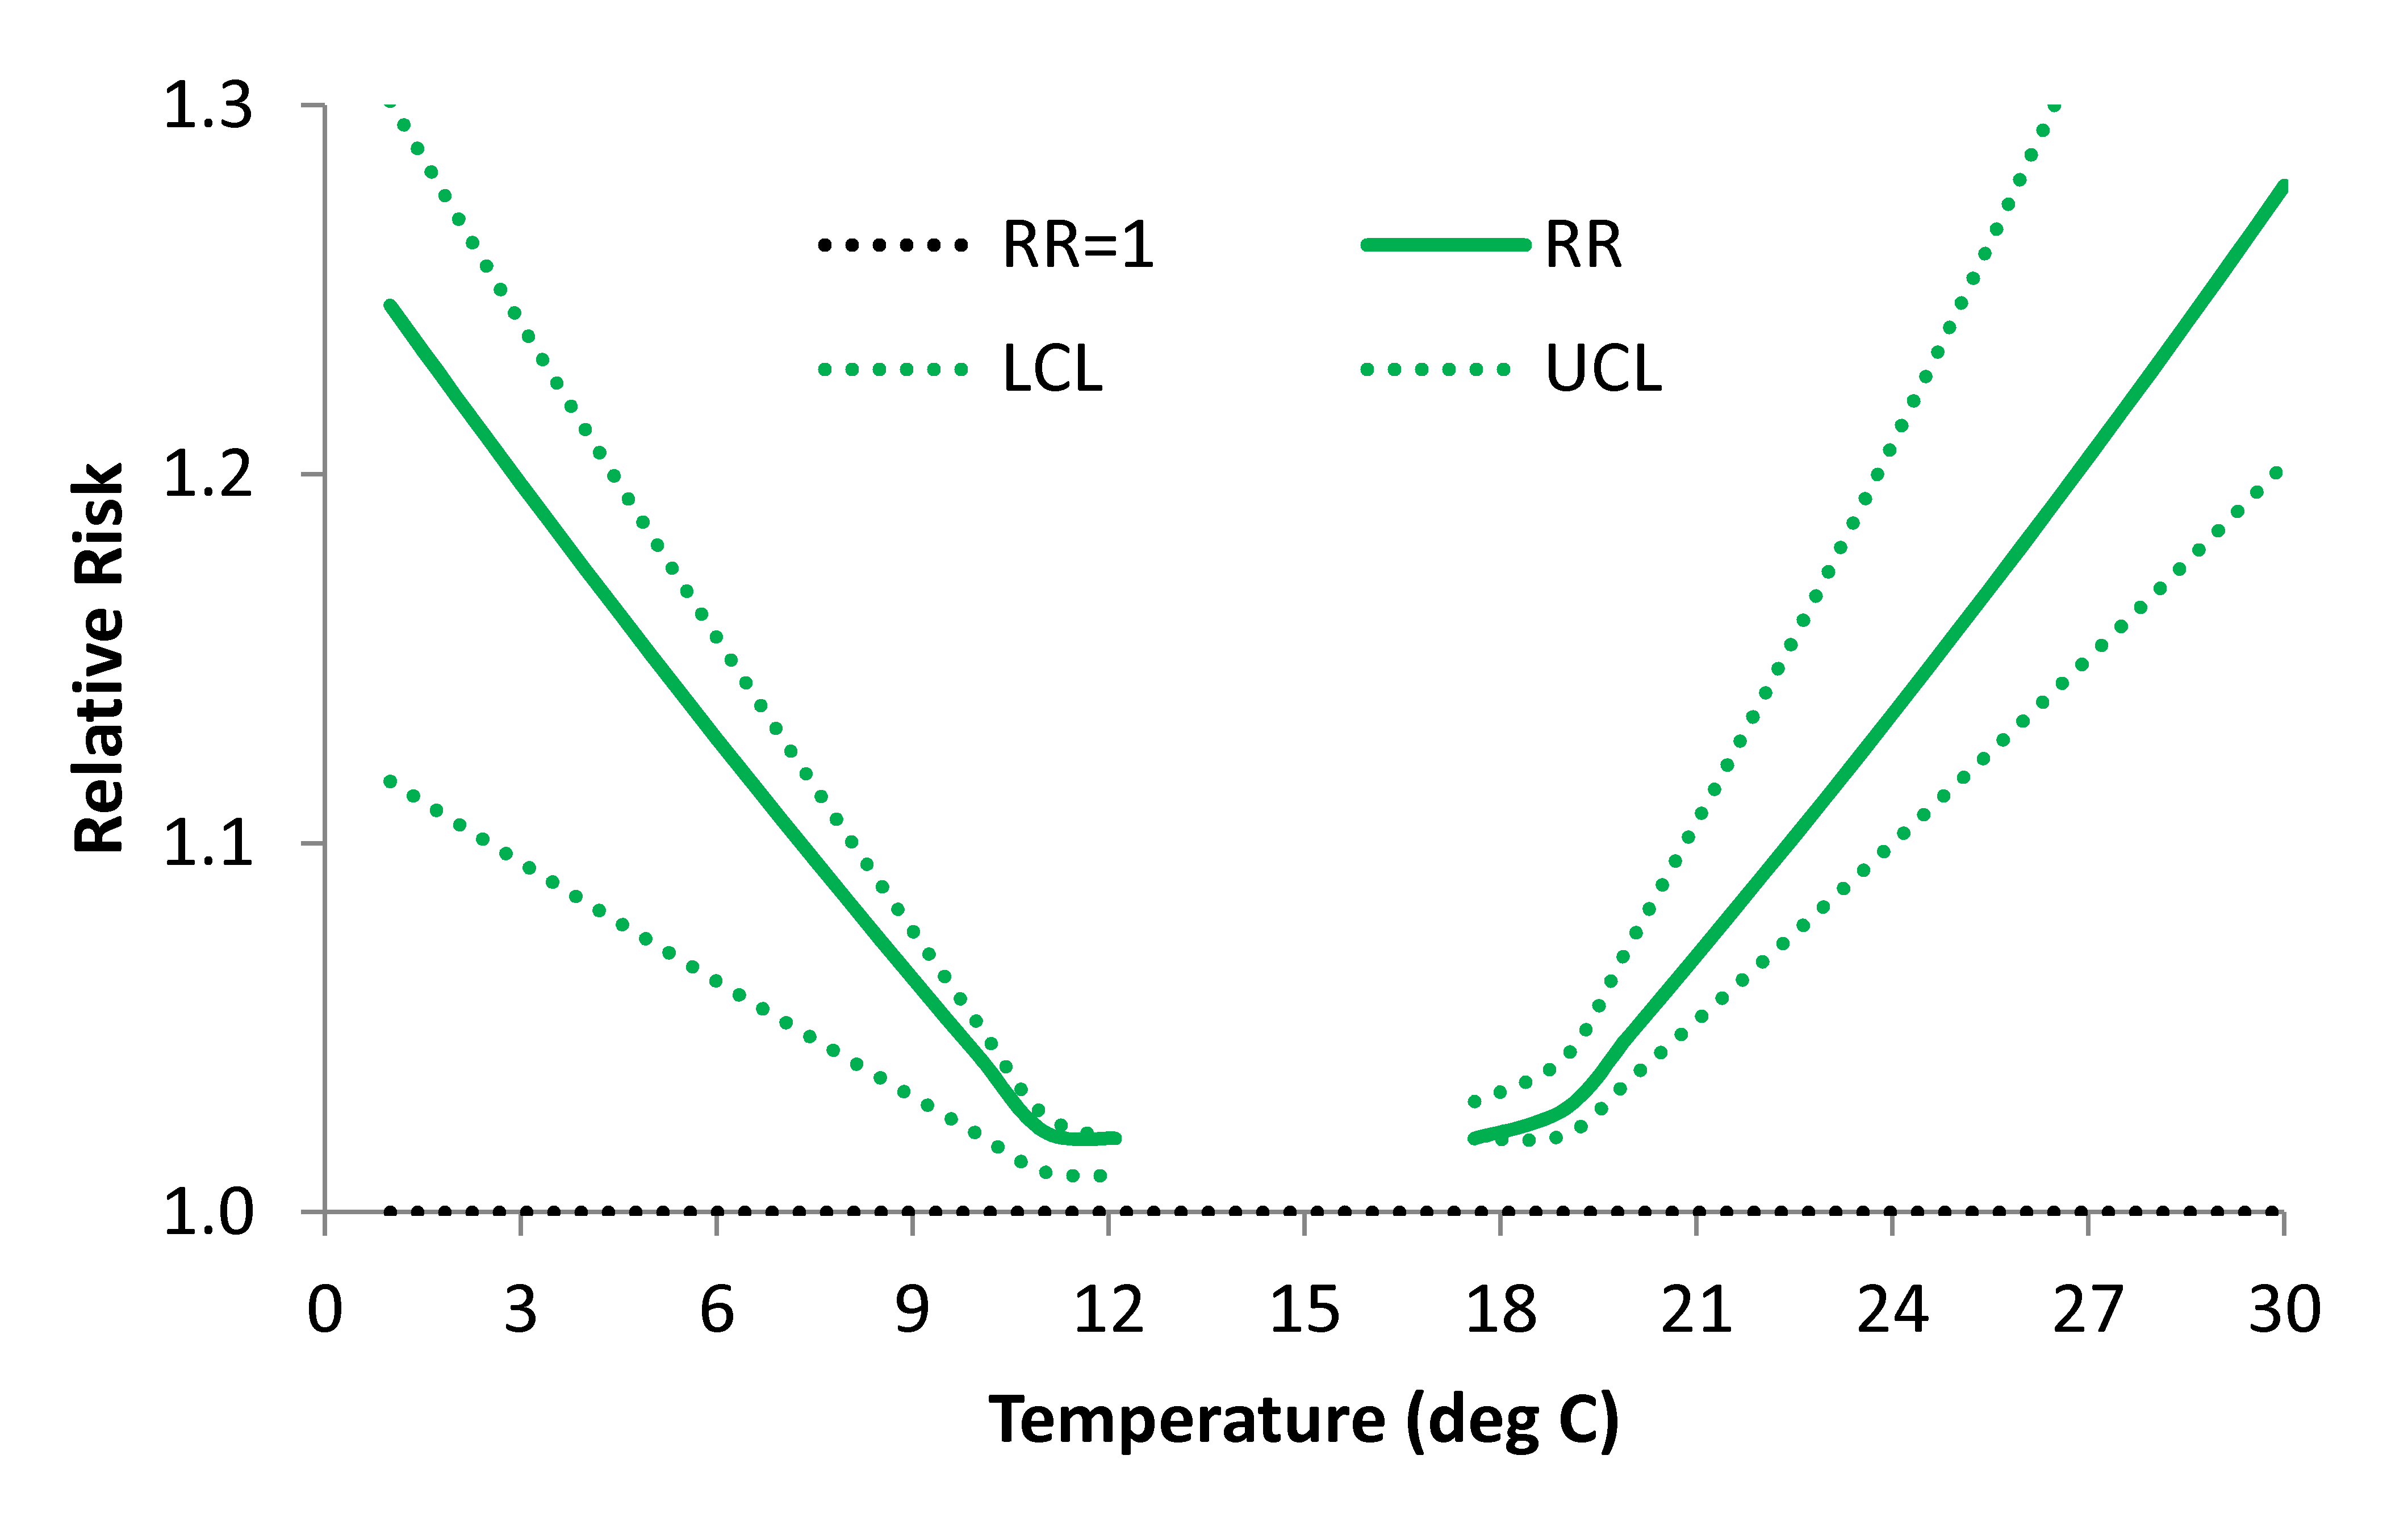
\includegraphics{CCA/img/RRgraph.png}
\caption[Relative Risk and Temperature]{The relative risk (RR) of death increases by approximately 2\% for each degree C beyond these thresholds.\label{fig:rr}}
\end{figure}





%\section{Climate Change}
\subsection{Climate Change Projections for UK}
This simulation model is based upon \href{http://ukclimateprojections.metoffice.gov.uk/media.jsp?mediaid=87867 \&filetype=pdf}{UKCP09 SRES A1B Emission Scenario Projection}, which "provides a basis for studies of impacts and vulnerability and decisions on adaptation to climate change in the UK over the 21st century."\cite{Jenkinsetal2009}

The emission 'story line' that underpins the future climate scenario used in this work is the IPCC's  \href{http://www.grida.no/publications/other/ipcc_sr/?src=/climate/ipcc/emission/}{Special Report Emissions Scenarios}.\cite{IPCC2000}

The Weather Generator is used here to provide a time series of mean daily temperature. It allows users to generate plausible daily time series at 5 km resolution level. As there is no climate change data available at the 5km scale, the Weather Generator 'downscales' the climate data from the 25km scale (Figure~\ref{fig:wgd}).\cite{Jonesetal2010}

\begin{figure}[htbp]
\centering
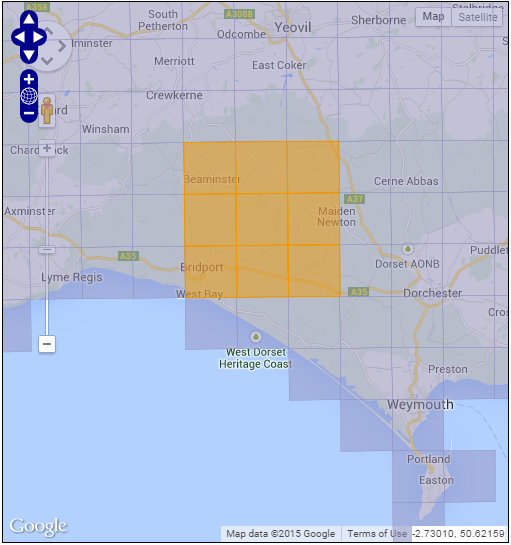
\includegraphics{CCA/img/WGD_WD.png}
\caption{Weather Generator spatial resolution over the West Dorset region.\label{fig:wgd}}
\end{figure}




%\section{Ageing Population}

\subsection{West Dorset Situation Population}
Dorset's population is ageing and this will have be a factor in how severely population health will be impacts by changing climate over the next 30 years. Population ageing, meaning that there will be a greater proportion of the population that is older in the future than is currently the case, is a global trend across the developed western world including the UK. There is a high degree of certainty that this trend will continue well beyond the 30 year reach of this study.

2012-based \href{www.ons.gov.uk/ons/rel/snpp/sub-national-population-projections/2012-based-projections/index.html}{Sub-national Population Projections} for Local Authorities in England, by sex and 5 year age groups, all local authorities and higher administrative areas within England Long-term sub-national population projections are an indication of the future trends in population by age and sex over the next 25 years.\cite{ons2012} They are trend-based projections, which means assumptions for future levels of births, deaths and migration are based on observed levels mainly over the previous five years. They show what the population will be if recent trends continue.

There are a number of uncertainties in ageing and the future of ageing in 2044 that we need to think carefully about:
\begin{itemize}
\item Quality of life, including increased fitness levels
\item Future work/retirement balance
\item Isolation and support for older people
\end{itemize}


\subsection{Public Health Interventions}
All public health interventions can be defined by three characteristics: the reach of the intervention (ie. who gets access to the intervention), who complies with the intervention, and what is the efficacy of the intervention.


%%%%  Section 2 Modelling
\section{Modelling for Public Health Intervention}



%\subsection{A Systems Dynamics Model}
A systems model was created using \url{insightmaker.com} to simulate the dynamics of temperature stress mortality in a warmer future West Dorset in 2044 (see Chapter on~\nameref{section:modelstory}). The model was developed with two objectives in mind:
\begin{itemize}
	\item To engage policy makers in a discussion about the potential health impacts of climate change on the health of our ageing population.
	\item To explore whether interactive systems models and associated story telling is a potentially effective tool in the policy development process and worth exploring further.
\end{itemize}

\subsection{How to use the model}
Follow this link: \href{https://insightmaker.com/insight/33655/Temperature-Stress-Mortality-Simulator}{Temperature Stress Mortality Simulator}\sidenote{insightmaker.com/insight/33655/ Temperature-Stress-Mortality-Simulator} to get the `guest login' that allows participants to change variables, simulation settings and run the simulation (Figure~\ref{fig:IMGuest}). The model starts in `story mode', which allows users to familiarise themselves with the model through a structured story using the `Step Forward' button located in the bottom-right corner of the screen.

There are four menu tabs along the top of the screen: Settings, Simulate, Tools, and Zoom, whose function will be obvious upon exploration. The best place to start -- click on the `Simulate' tab and explore the model output.

The model variables are provided along the right-hand-side of the screen and can be scrolled through to review and each variable can be set with easy to use `slider bars'.
\begin{description}
	\item [Age Groups] Choose the age groups or everyone over 70 years (All)
	\item [Sex] Older men have a significantly higher base mortality rate
	\item [SEC] Socio-economic class has a significant impact on base mortality rates and on simulation results
	\item [Reach] Defining the public health intervention
	\item [Efficacy] Defining the public health intervention
	\item [Intervention Target] Define the thermal stress in which to intervene
	\item [Compliance] Defining the public health intervention
\end{description}

Folders, box elements with a `+' in the top-left corner contain further information and model parameters. 

Further information about any element in the model can be had by a left-mouse click on that element. The additional information will be presented on the right-hand side of the screen, and at the bottom of this panel, users can explore systems thinking concepts represented by the element.

Additionally, when you move the pointer over an element an `i' and a `folder' symbol will appear and each of these will also provide further information about that element.

\begin{figure*}[htbp]
	\centering
	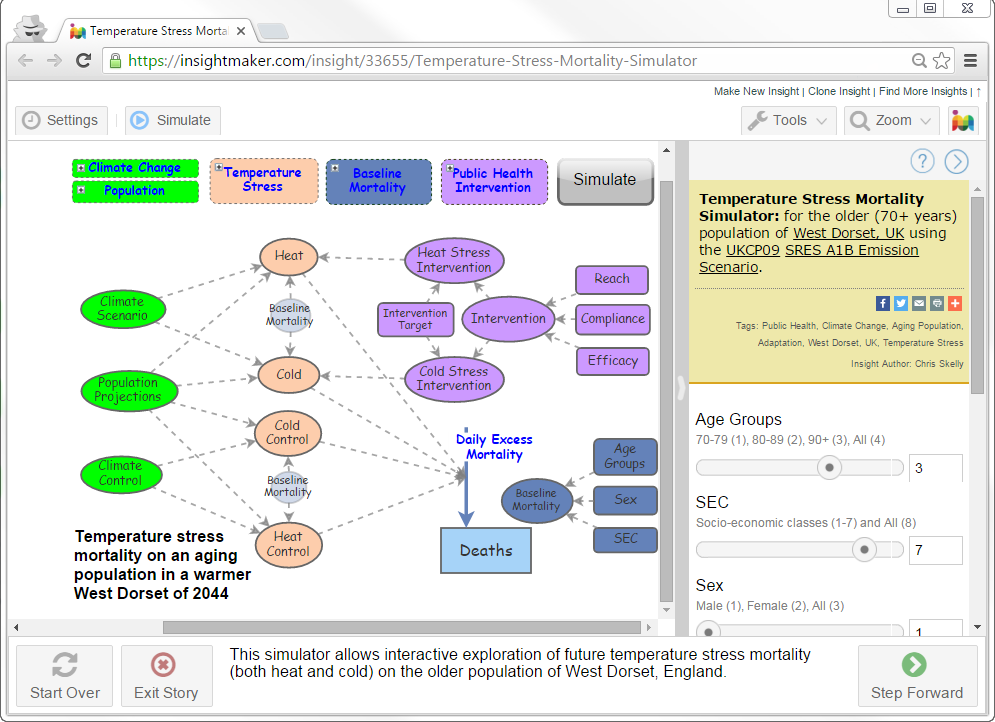
\includegraphics{./CCA/img/InsightMaker_GuestScreen.png}
	\caption[Insight Maker Guest Login Screen]{Users of our system model ``Temperature Stress Mortality Simulator'' will be presented with this user interface if they follow the provided link. Note that there are now more menu tabs along the top of the screen: add primitives, flows/transitions/links, edit, style. These tabs contain the tools for editing and creating models.\label{fig:IMGuest}}
\end{figure*}

\subsection{How to modify the model}
Follow this link: \href{https://insightmaker.com/}{Insight Maker}\sidenote{https://insightmaker.com/} to get to the page that allows participants to set up an account, explore other people's models and create your own (Figure~\ref{fig:IMLogin}).

\begin{description}
	\item [Create account] `Create a Free Account' -- top-right of screen
	\item [Search for Model] `Explore Insights' --> `Find Insights' --> `Search': Temperature Stress Mortality Simulator
	\item [Copy Model] Select model --> Clone Insight (top-right menu)\sidenote{You now have your own copy of the model and you can make any modifications to it that you like.}
\end{description}

\begin{figure*}[htbp]
	\centering
	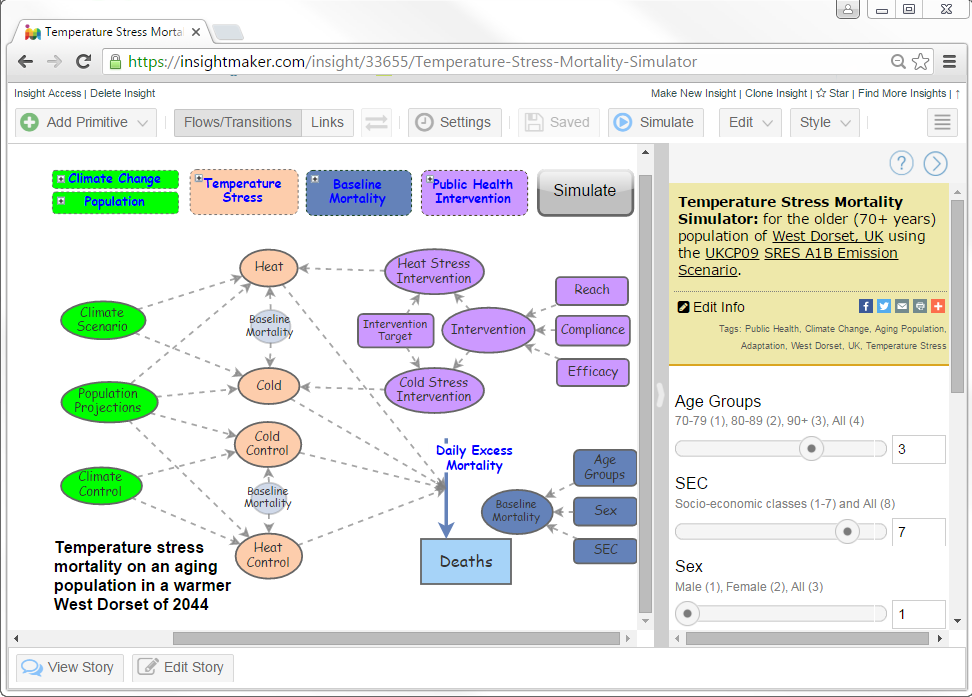
\includegraphics{./CCA/img/InsightMaker_LoggedinScreen.png}
	\caption[Insight Maker User Login Screen]{Users of our system model ``Temperature Stress Mortality Simulator'' will be presented with this user interface if they create a free account and make a copy of the model.\label{fig:IMLogin}}
\end{figure*}

\subsection{Story Telling} \label{section:modelstory}
The `model story' is an interactive tour of the system model developed for this project that was produced using \href{https://insightmaker.com}{Insight Maker}\sidenote{insightmaker.com/}. The story is available online allowing direct interaction with the model \href{https://insightmaker.com/insight/33655/Temperature-Stress-Mortality-Simulator}{Temperature Stress Mortality Simulator}\sidenote{insightmaker.com/insight/33655/ Temperature-Stress-Mortality-Simulator}.

By Chris Skelly\\
June 20, 2015
\begin{description}
	\item[Temperature Stress Mortality Simulator:] for the older (70+ years) population of~\href{http://en.wikipedia.org/wiki/West\_Dorset}{West Dorset, UK}\sidenote{en.wikipedia.org/wiki/West\_Dorset}~using the~\href{http://ukclimateprojections.metoffice.gov.uk/}{UKCP09}\sidenote{ukclimateprojections.metoffice.gov.uk}~\href{http://www.grida.no/publications/other/ipcc\_sr/?src=/climate/ipcc/emission/}{SRES A1B Emission Scenario}\sidenote{www.grida.no/publications/other/ ipcc\_sr/?src=/climate/ipcc/emission/}.
	\item[Acknowledgements] We would like to thank Communities Living Sustainably for funding this project from a Big Lotteries grant and all my colleagues at Dorset Public Health who made this project happen --- Chris Ricketts wrote the proposal and guided its early development, Rebecca Pearce managed the project and Dave Lemon undertook the modelling work to adapt temperature stress to West Dorset.
\end{description}

\begin{figure}[tb]
	\centering
	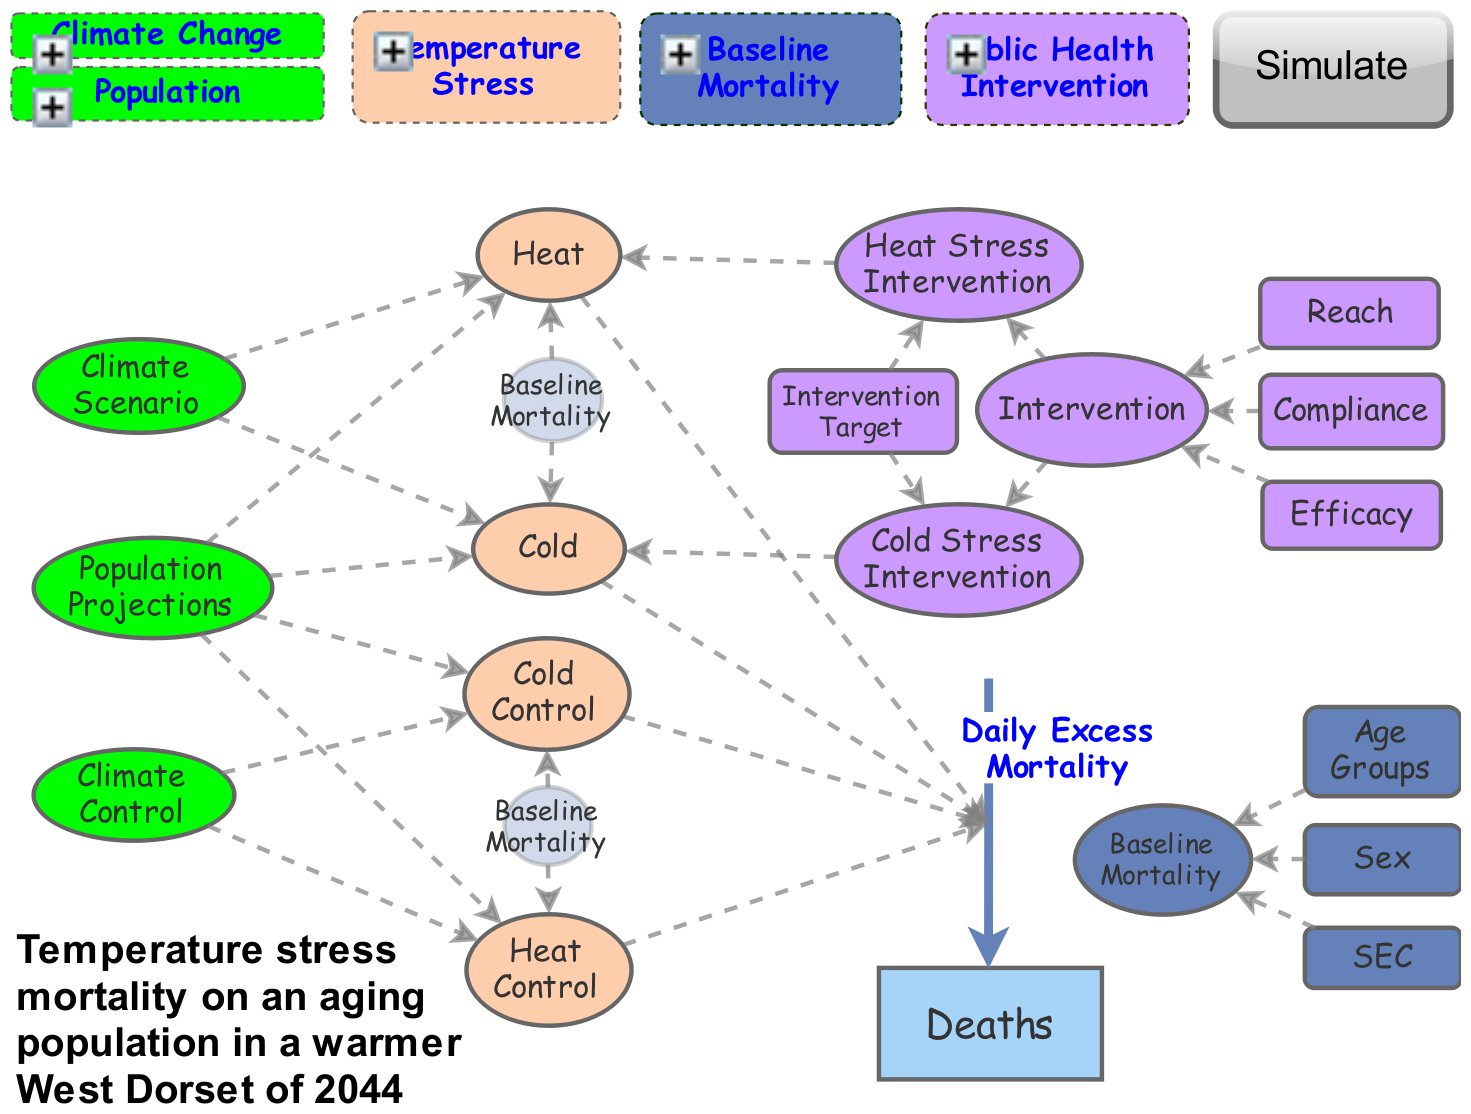
\includegraphics{./CCA/img/image_1.png}
	\caption[System Model Simulator]{This simulator allows interactive exploration of future temperature stress mortality (both heat and cold) on the older population of West Dorset, England.}
\end{figure}

\begin{figure}[htbp]
	\centering
	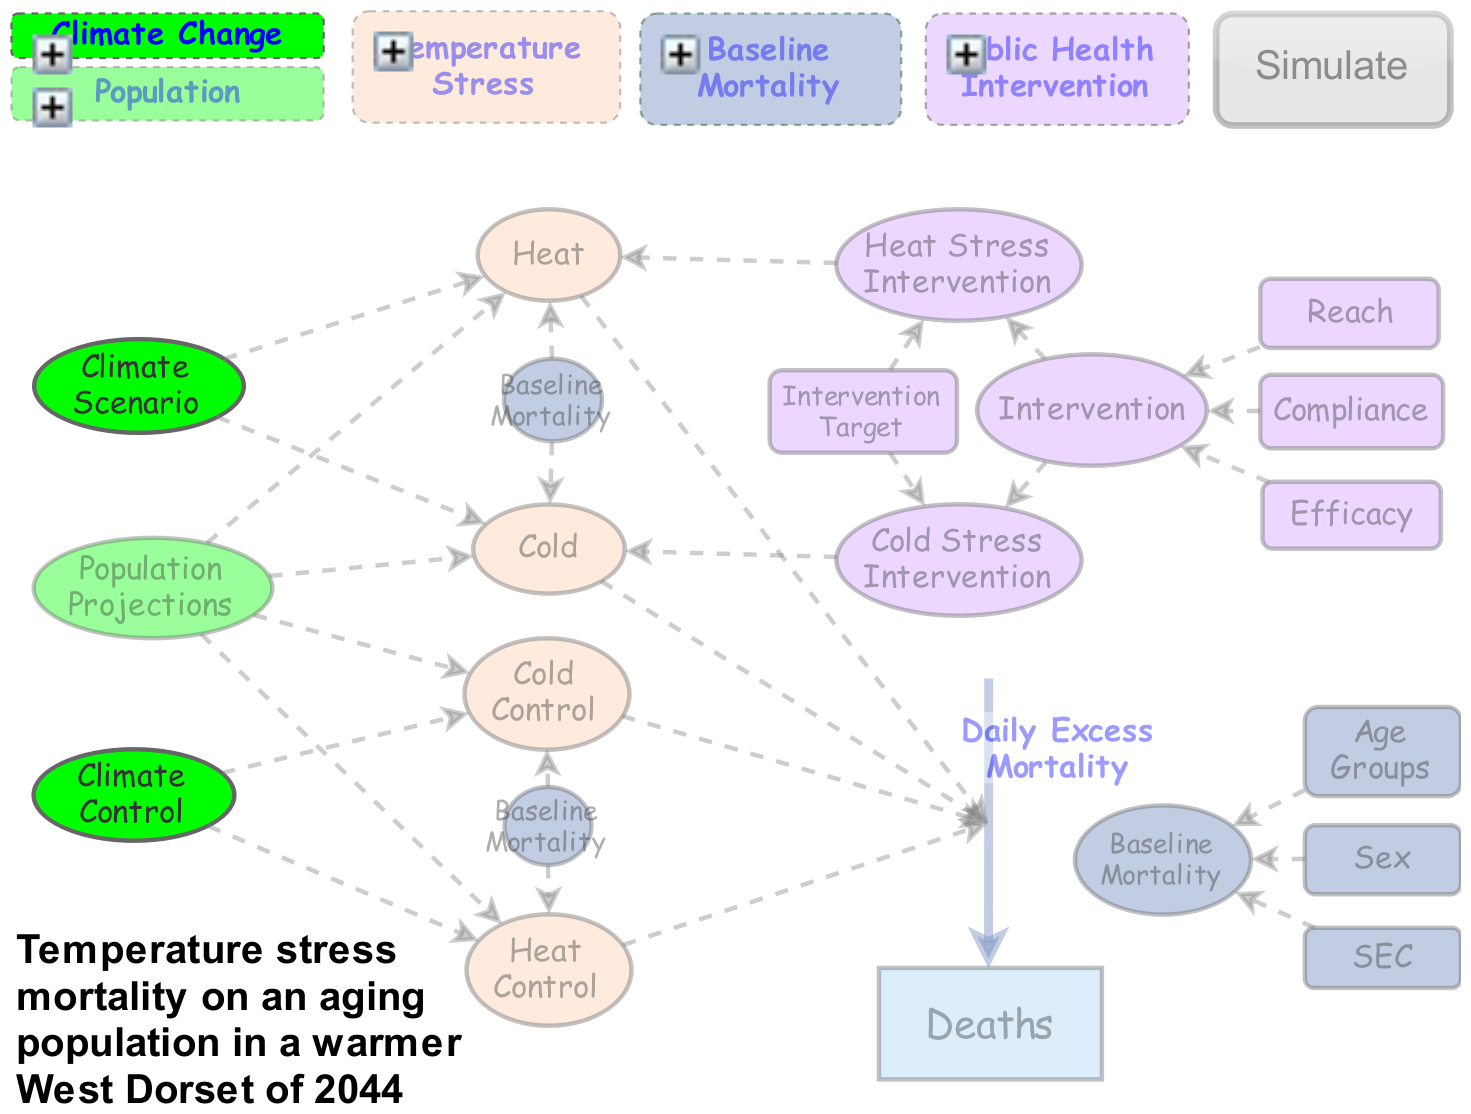
\includegraphics{./CCA/img/image_2.png}
	\caption[UKCP09 Scenario Data]{This simulator is driven using a future climate scenario (UKCP09) that is the basis of much climate adaptation policy in the United Kingdom. It is `downscaled' to the West Dorset region producing plausible daily temperature values for both the climate scenario (2044) and a control period (contemporary observed climate).}
\end{figure}

\begin{figure}[htbp]
	\centering
	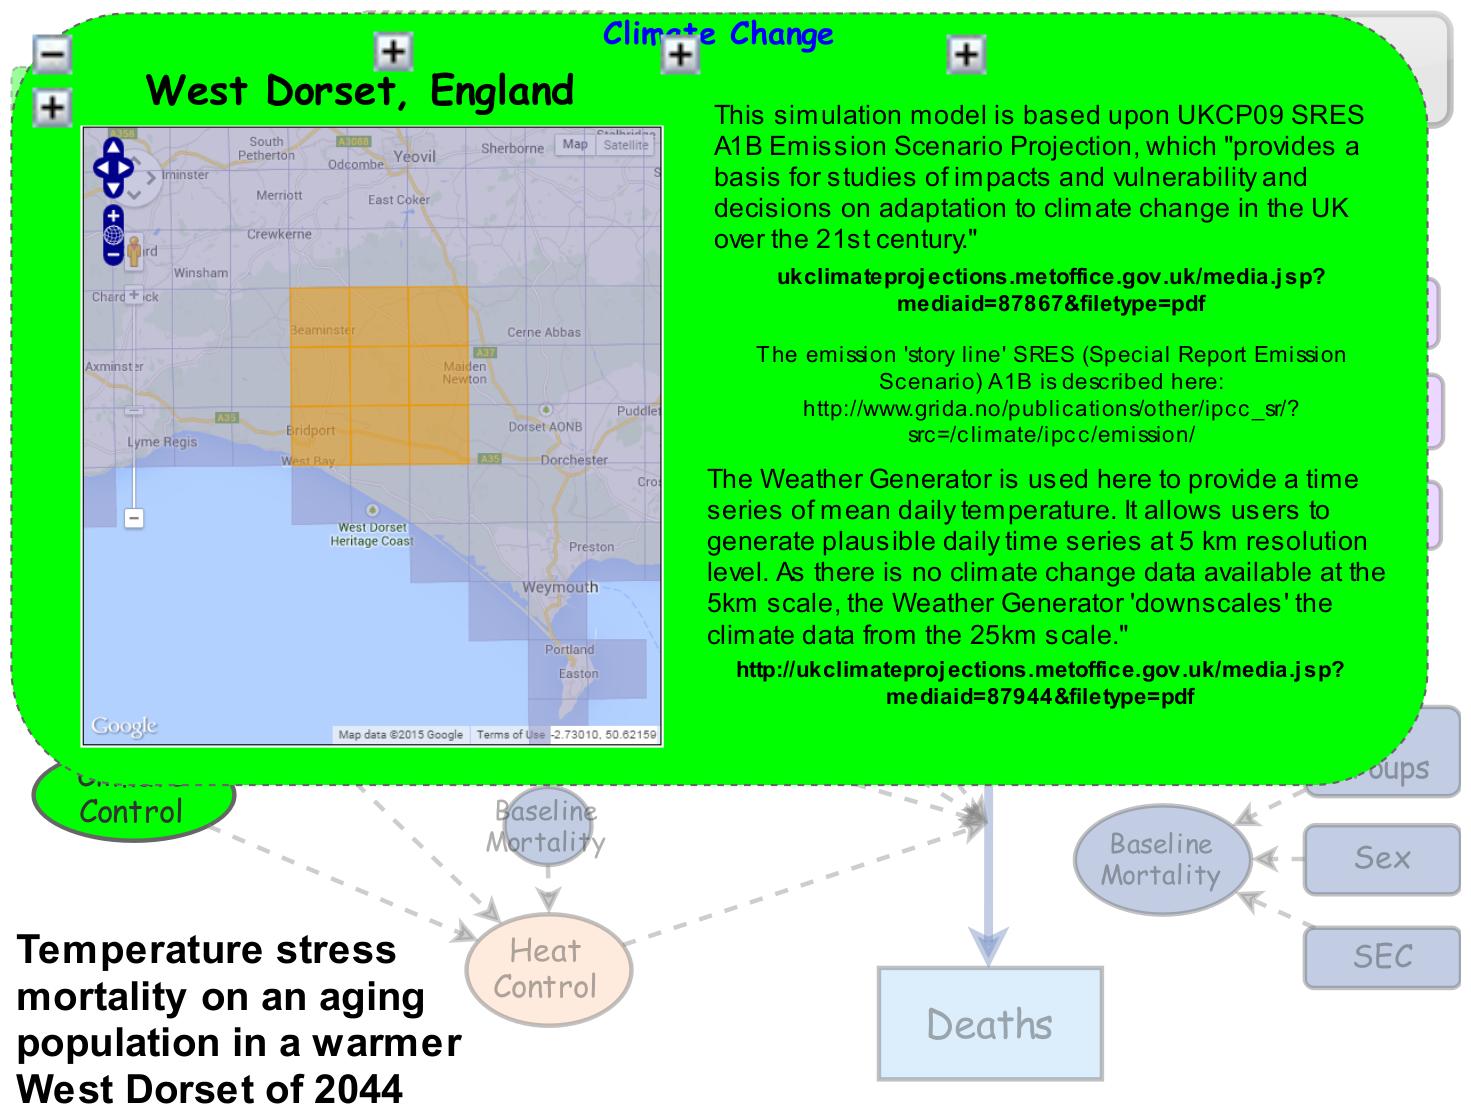
\includegraphics{./CCA/img/image_3.png}
	\caption[Simulated Climate Data]{Simulated climate data and scenarios details are found here.}
\end{figure}

\begin{figure}[htbp]
	\centering
	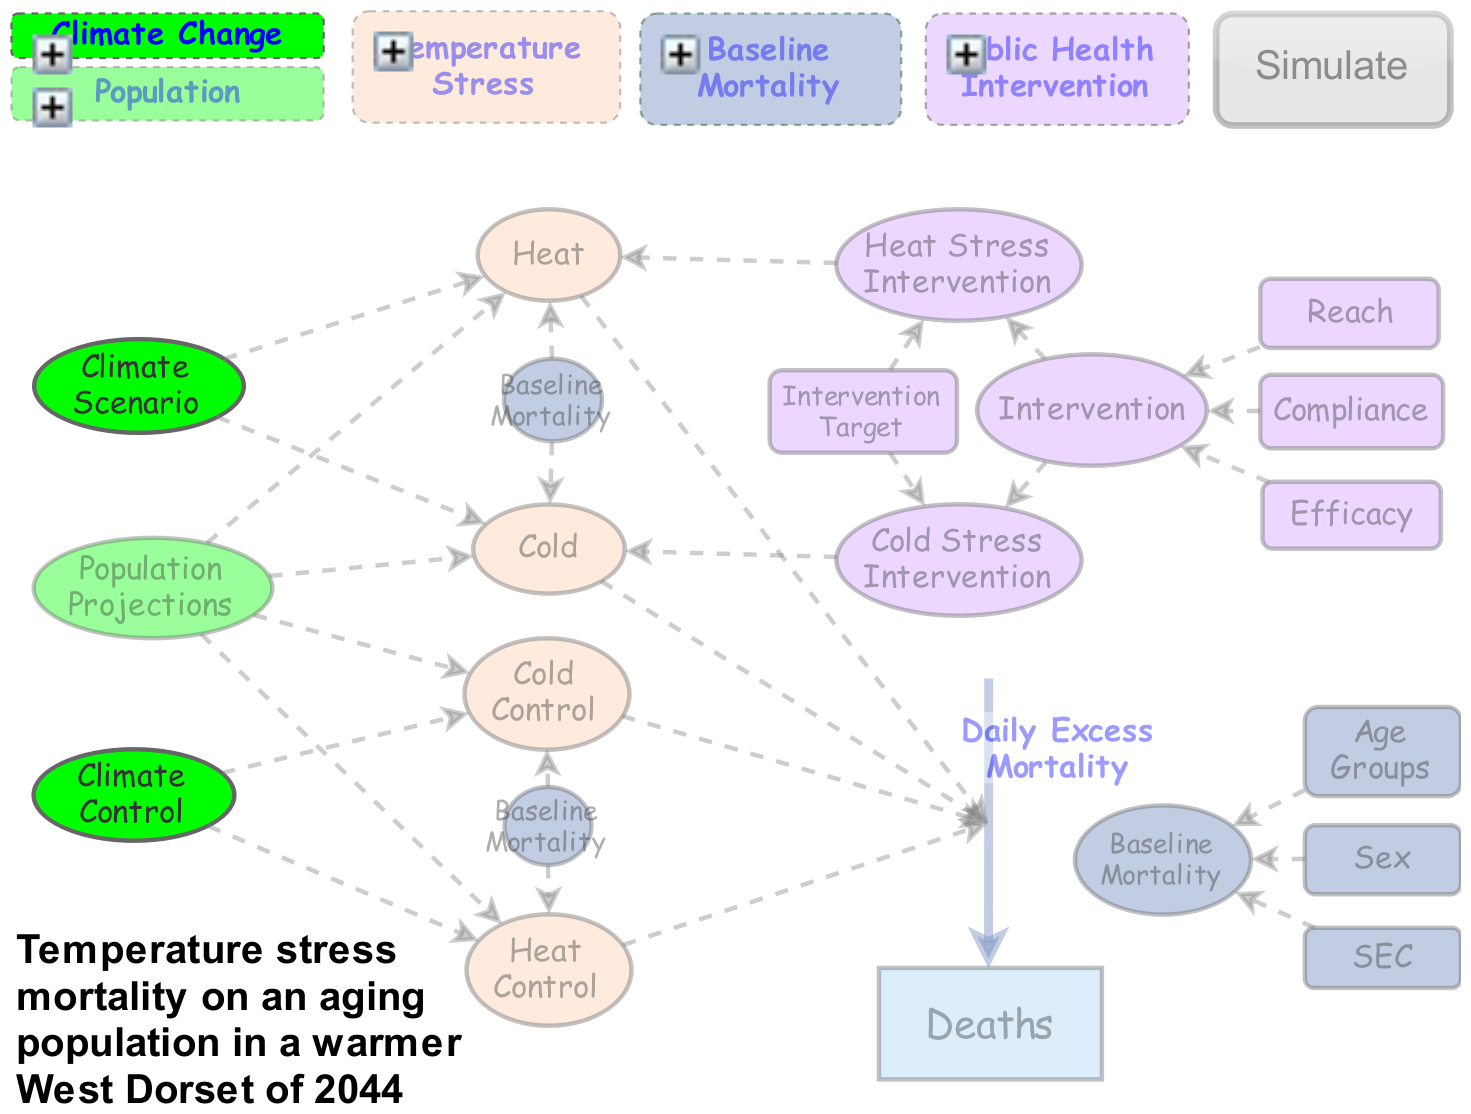
\includegraphics{./CCA/img/image_4.png}
	\caption[Population Change in West Dorset]{The climate is not the only thing that is forecast to change in West Dorset by 2044\ldots}
\end{figure}

\begin{figure}[htbp]
	\centering
	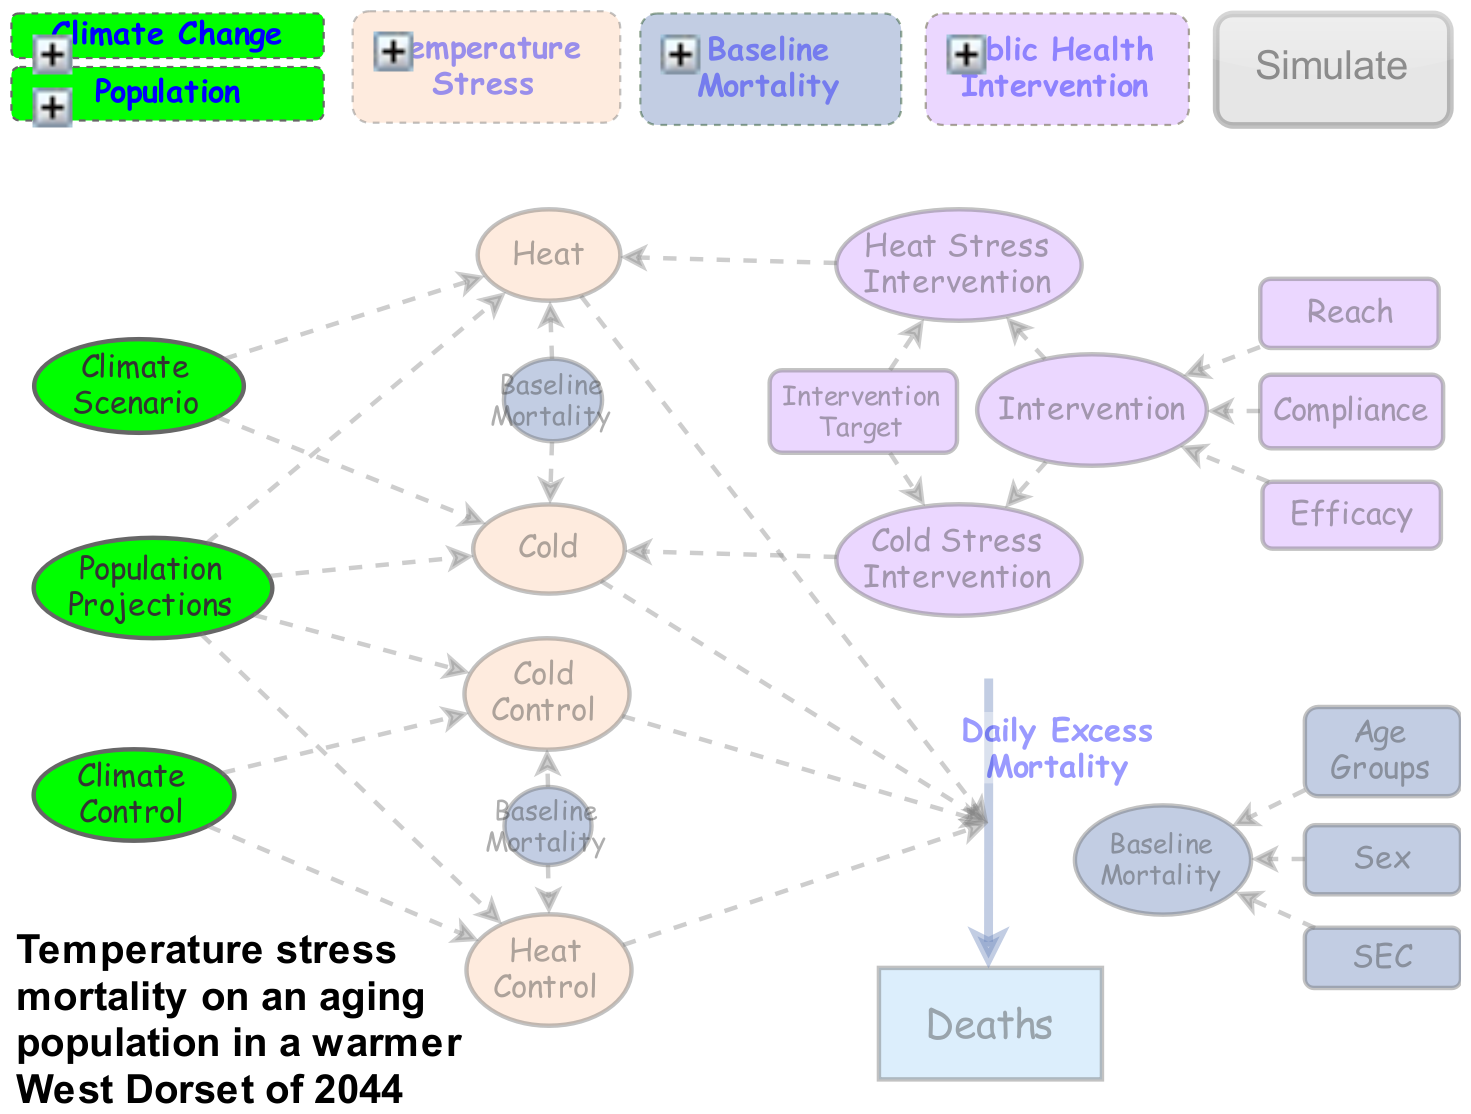
\includegraphics{./CCA/img/image_5.png}
	\caption[Ageing West Dorset Population]{The population of West Dorset, like that of the United Kingdom is ageing. In addition to an ageing population, there has been a retirement migration movement to the Dorset region for many years. This is likely to continue.}
\end{figure}

\begin{figure}[htbp]
	\centering
	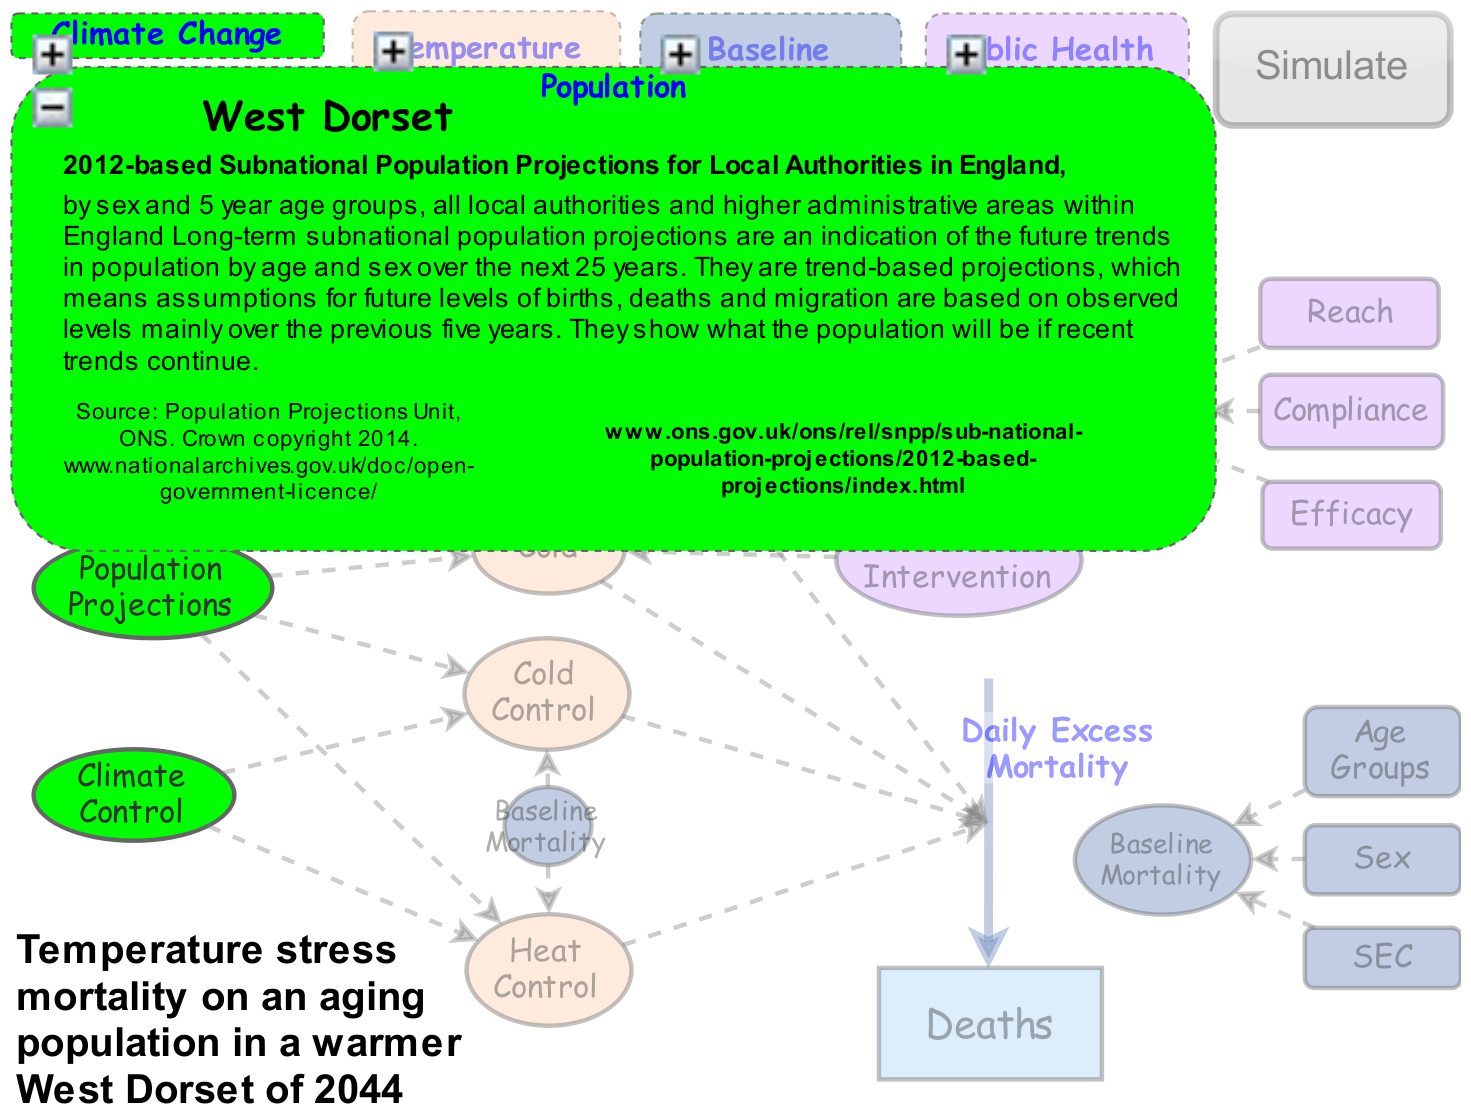
\includegraphics{./CCA/img/image_6.png}
	\caption[ONS Population Projections]{Population projection data, from the~Office of National Statistics, is detailed in this folder.}
\end{figure}

\begin{figure}[htbp]
	\centering
	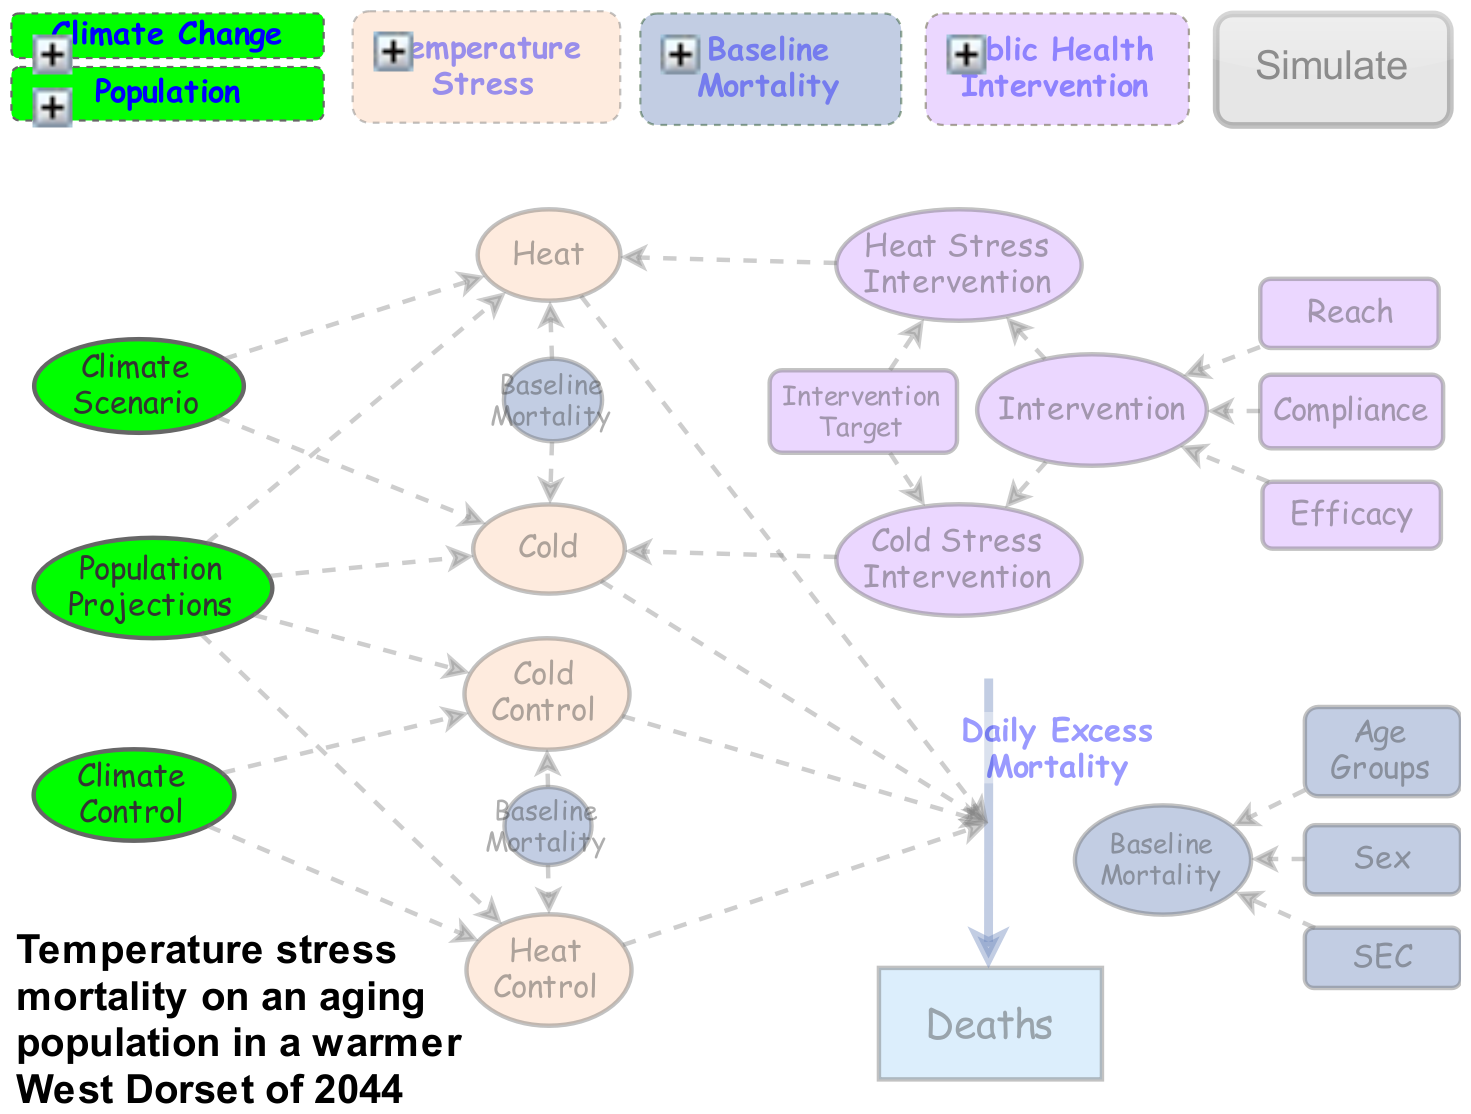
\includegraphics{./CCA/img/image_7.png}
	\caption[Climate Warming and Population Ageing]{The climate is expected to warm and the population is expected to age.}
\end{figure}

\begin{figure}[htbp]
	\centering
	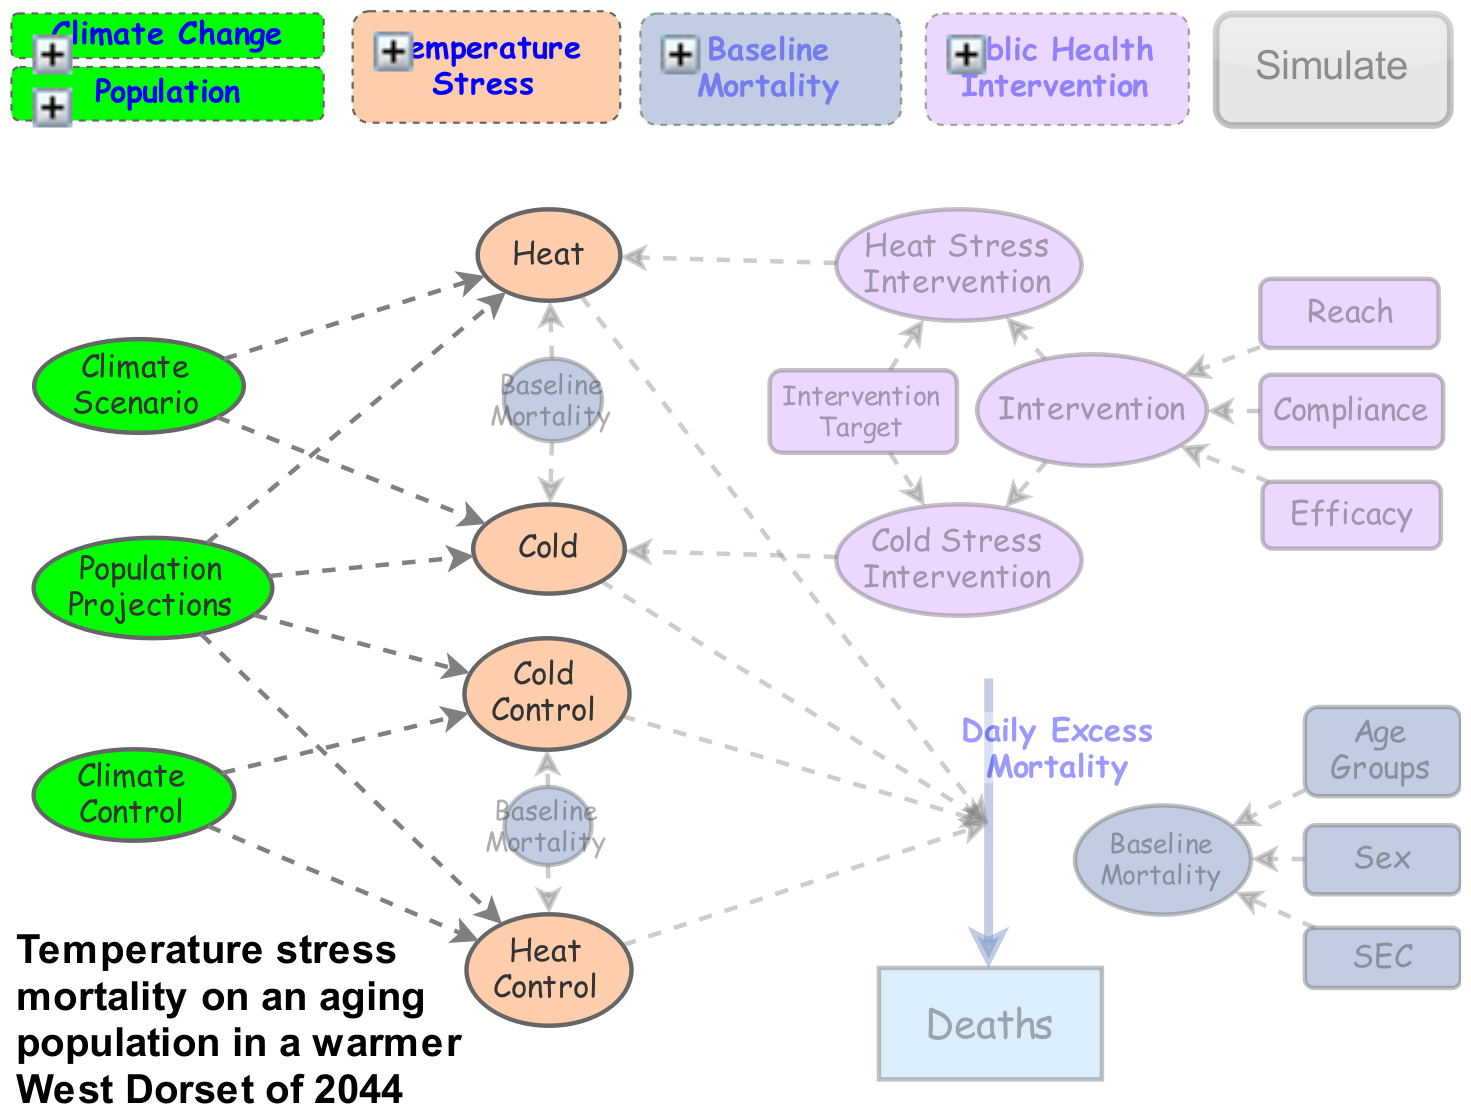
\includegraphics{./CCA/img/image_8.png}
	\caption[Thermal Stress]{Human physiology responds to ambient temperatures. If it is too warm or too cold the human body is stressed. This is most noticeable during major heatwaves when most of the population can feel the `heat stress'.}
\end{figure}

\begin{figure}[htbp]
	\centering
	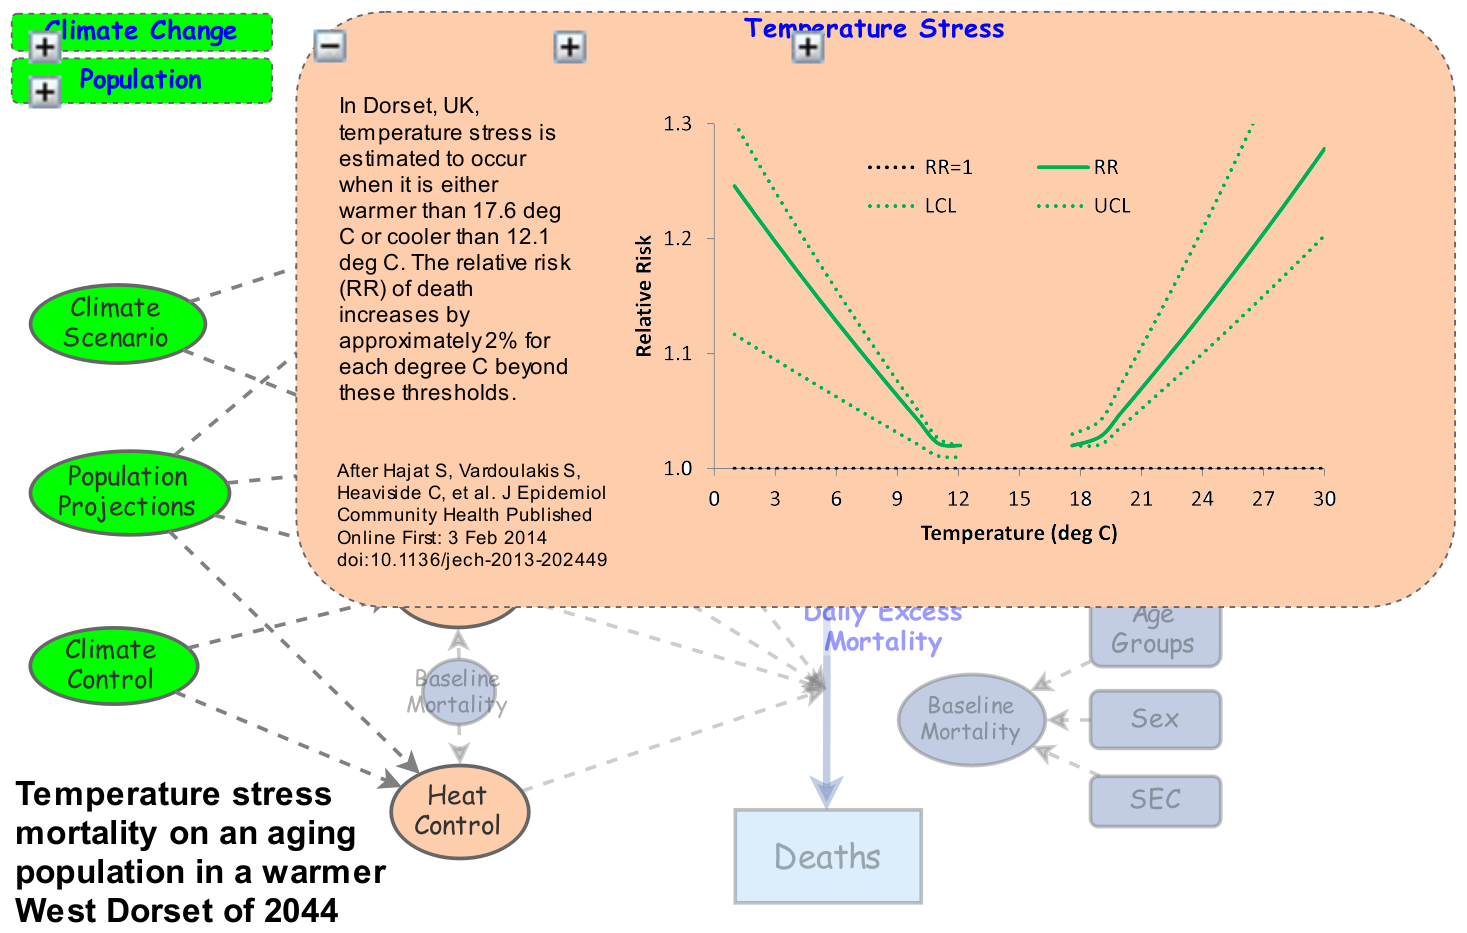
\includegraphics{./CCA/img/image_9.png}
	\caption[Thermal Stress Thresholds]{However, temperature stress occurs far more frequently than we might think -- and in Dorset at almost any time of year. Additionally, as we age, we tend to `feel' the cold or heat more. In other words, we experience more temperature stress. We have adapted a model that estimates the mortality associated with temperature stress in the West Dorset climate. It uses a `base mortality rate' (more on this later) for a population to estimate the temperature stress related `excess mortality'. This model shows that for every 1 degree C in temperature over either a heat or cold threshold excess mortality increases by 2\%. This is the fundamental relationship upon which this simulator is based.}
\end{figure}

\begin{figure}[htbp]
	\centering
	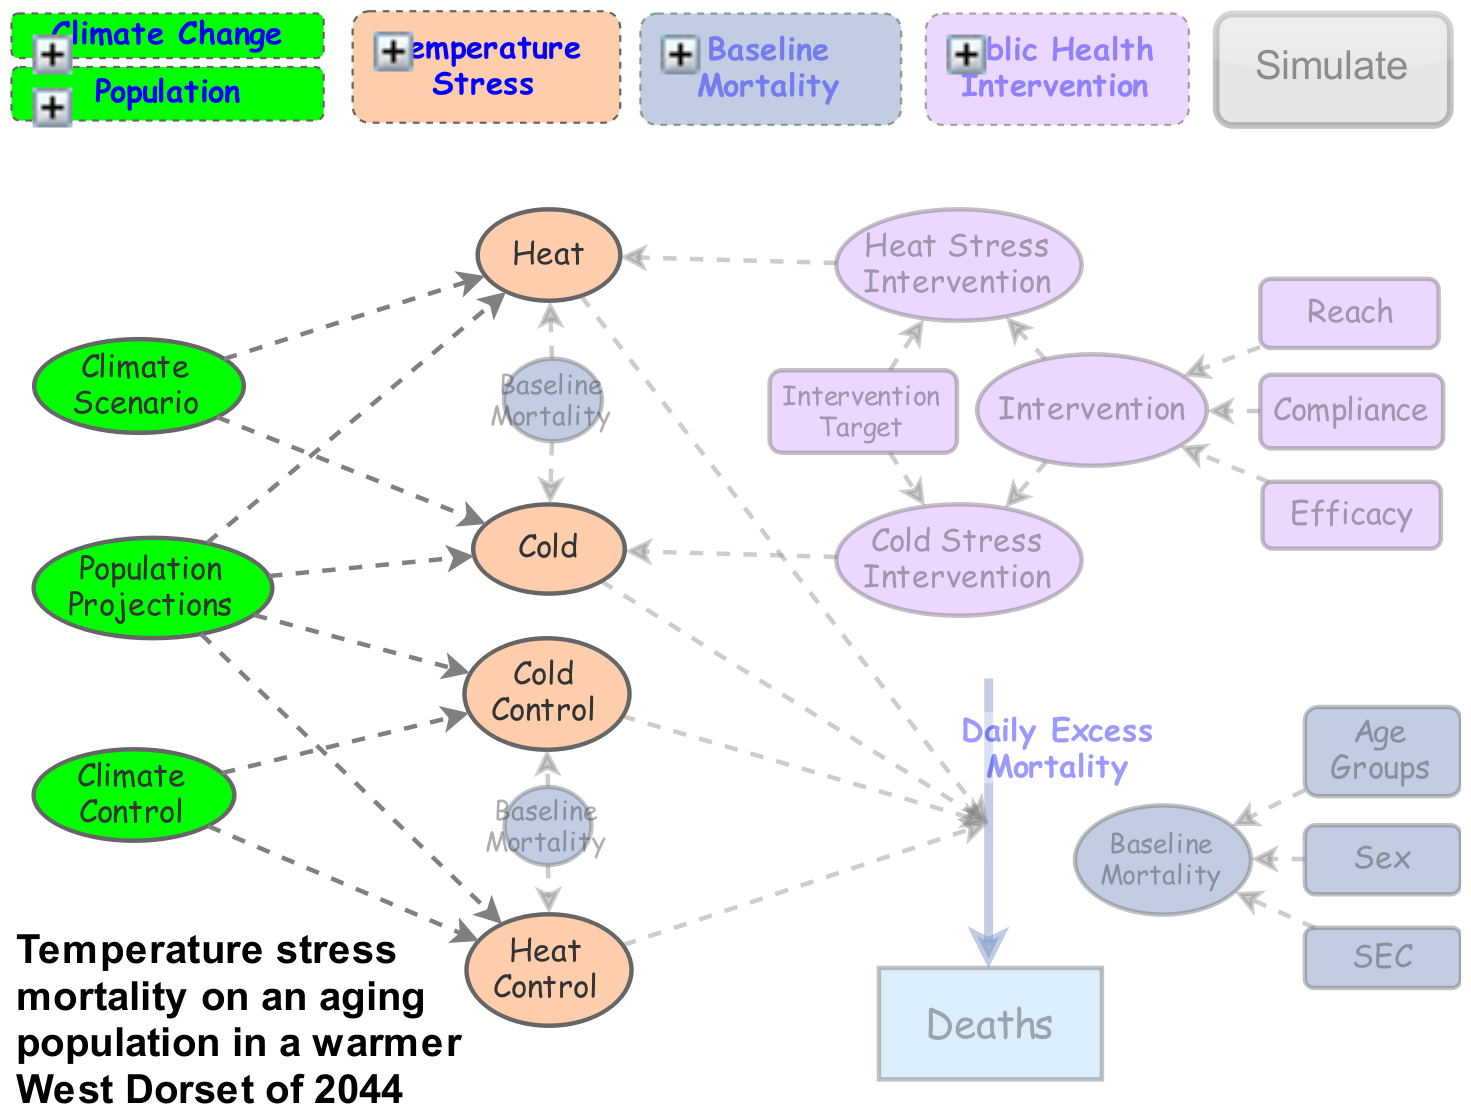
\includegraphics{./CCA/img/image_10.png}
	\caption[Base Mortality Rates]{The relationship between temperature and the base mortality rate is how we define `temperature stress'. But where do these `base mortality rates' come from?}
\end{figure}

\begin{figure}[htbp]
	\centering
	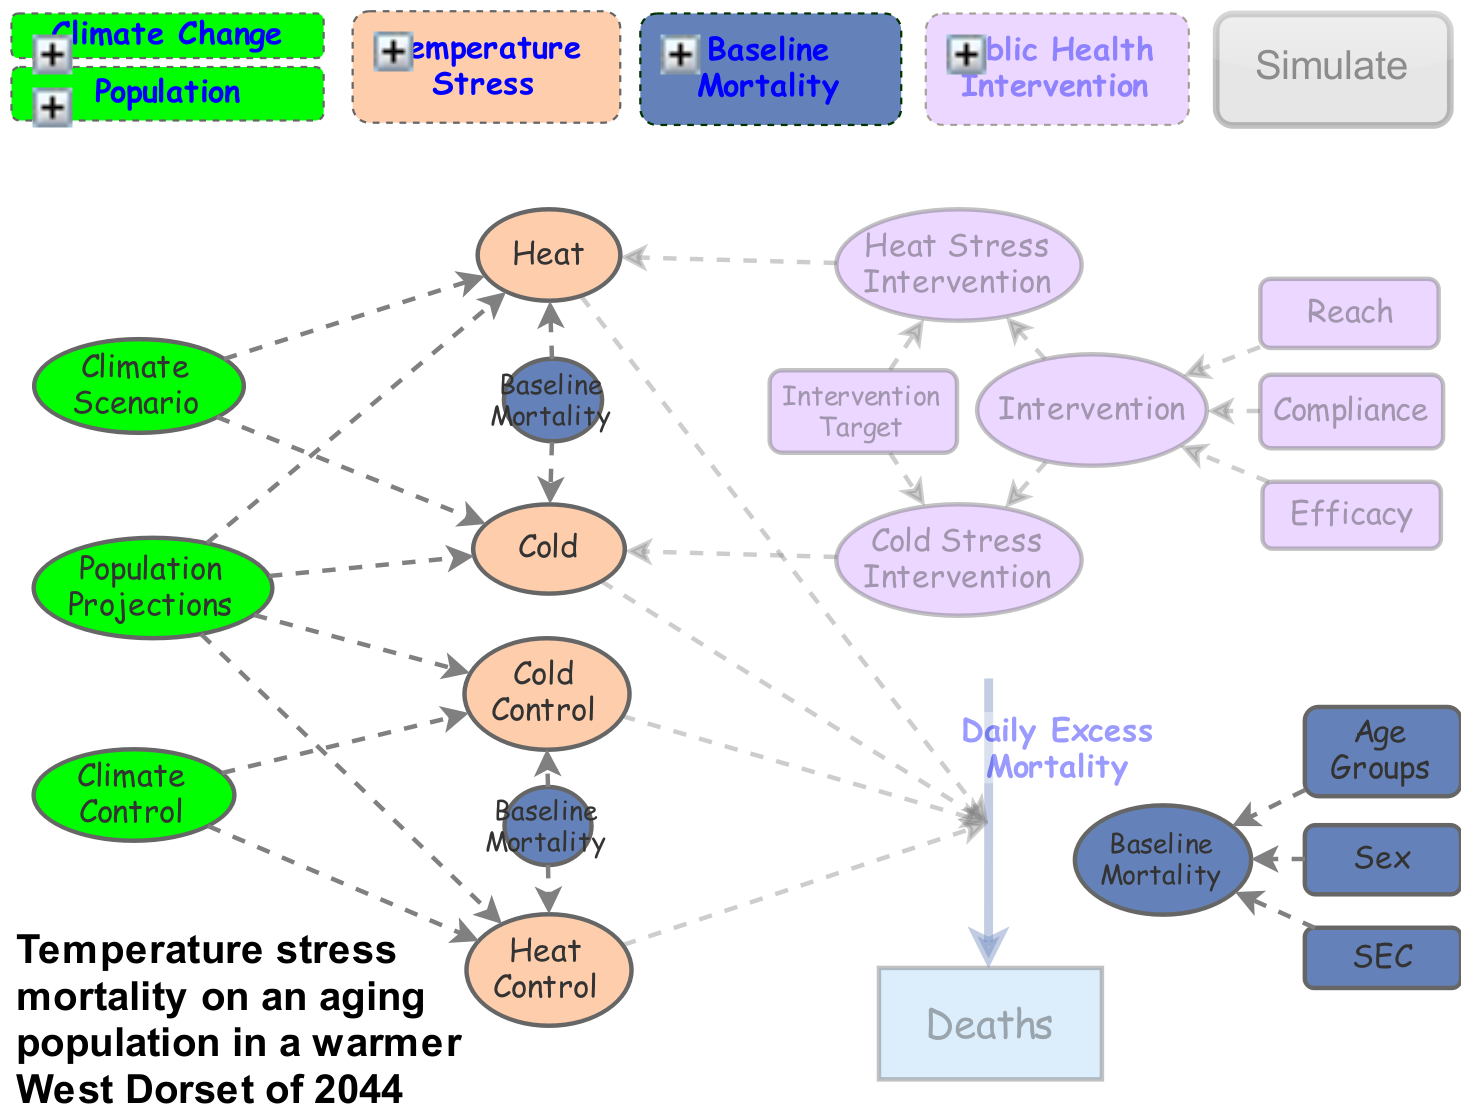
\includegraphics{./CCA/img/image_11.png}
	\caption[Age Specific Base Mortality Rates]{Base mortality rates are produced in the United kingdom for different groups by age, gender and socio-economic class (SEC), because it is well established that there are significant inequalities across these groups.}
\end{figure}

\begin{figure}[htbp]
	\centering
	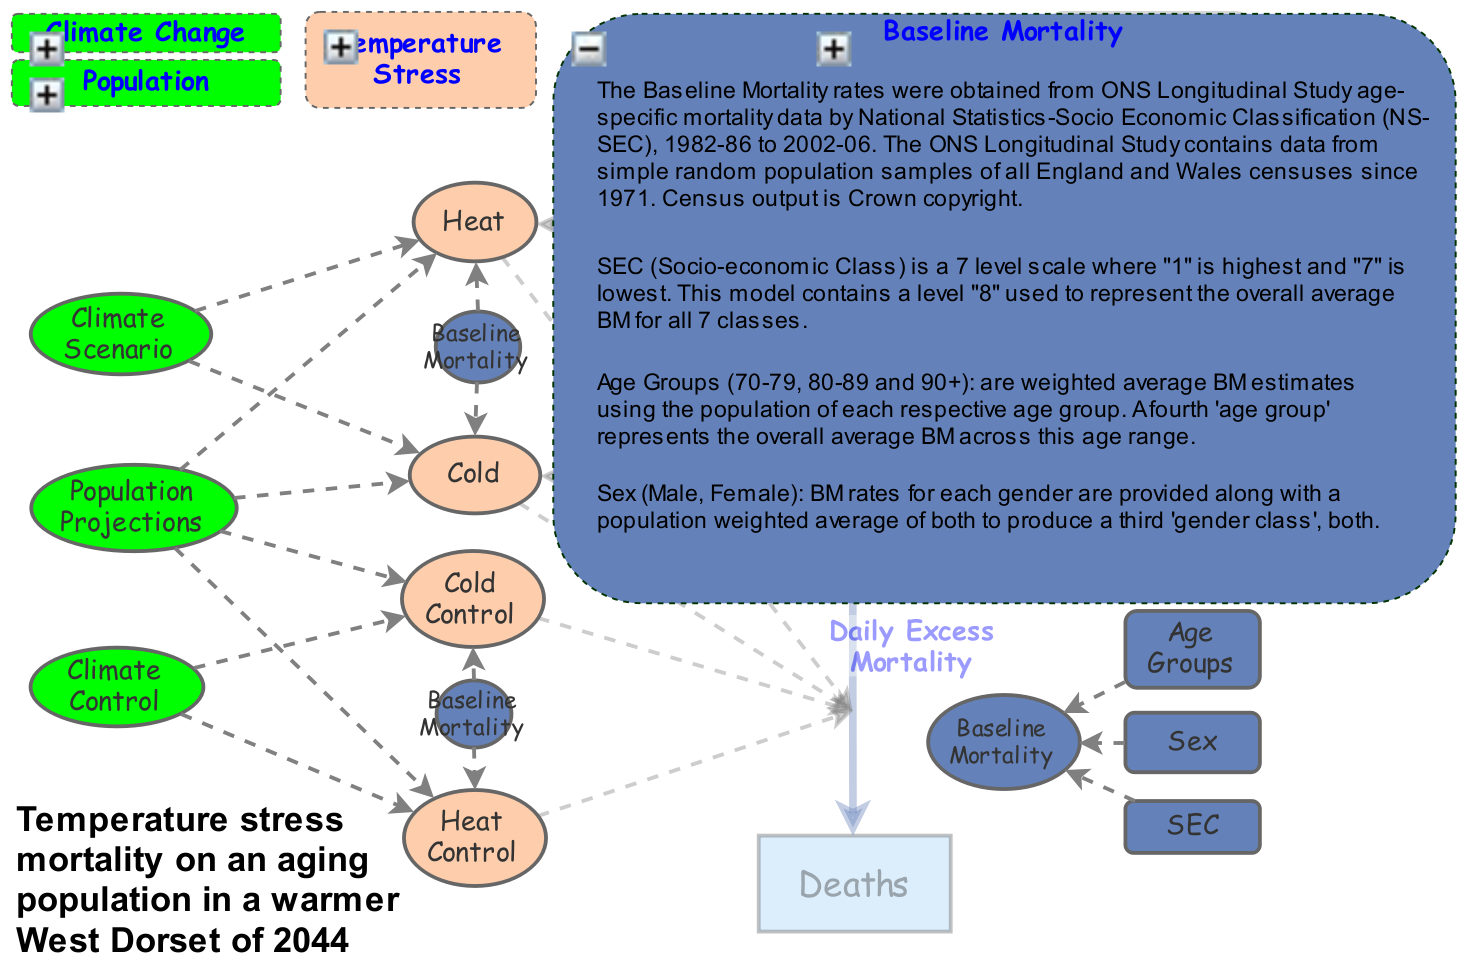
\includegraphics{./CCA/img/image_12.png}
	\caption[Population Variables]{This simulator allows the user to set the age group (4 groups for the over 70+ population are available), sex and socio-economic class (SEC 1-7 is from highest to lowest and 8 is for all classes).}
\end{figure}

\begin{figure}[htbp]
	\centering
	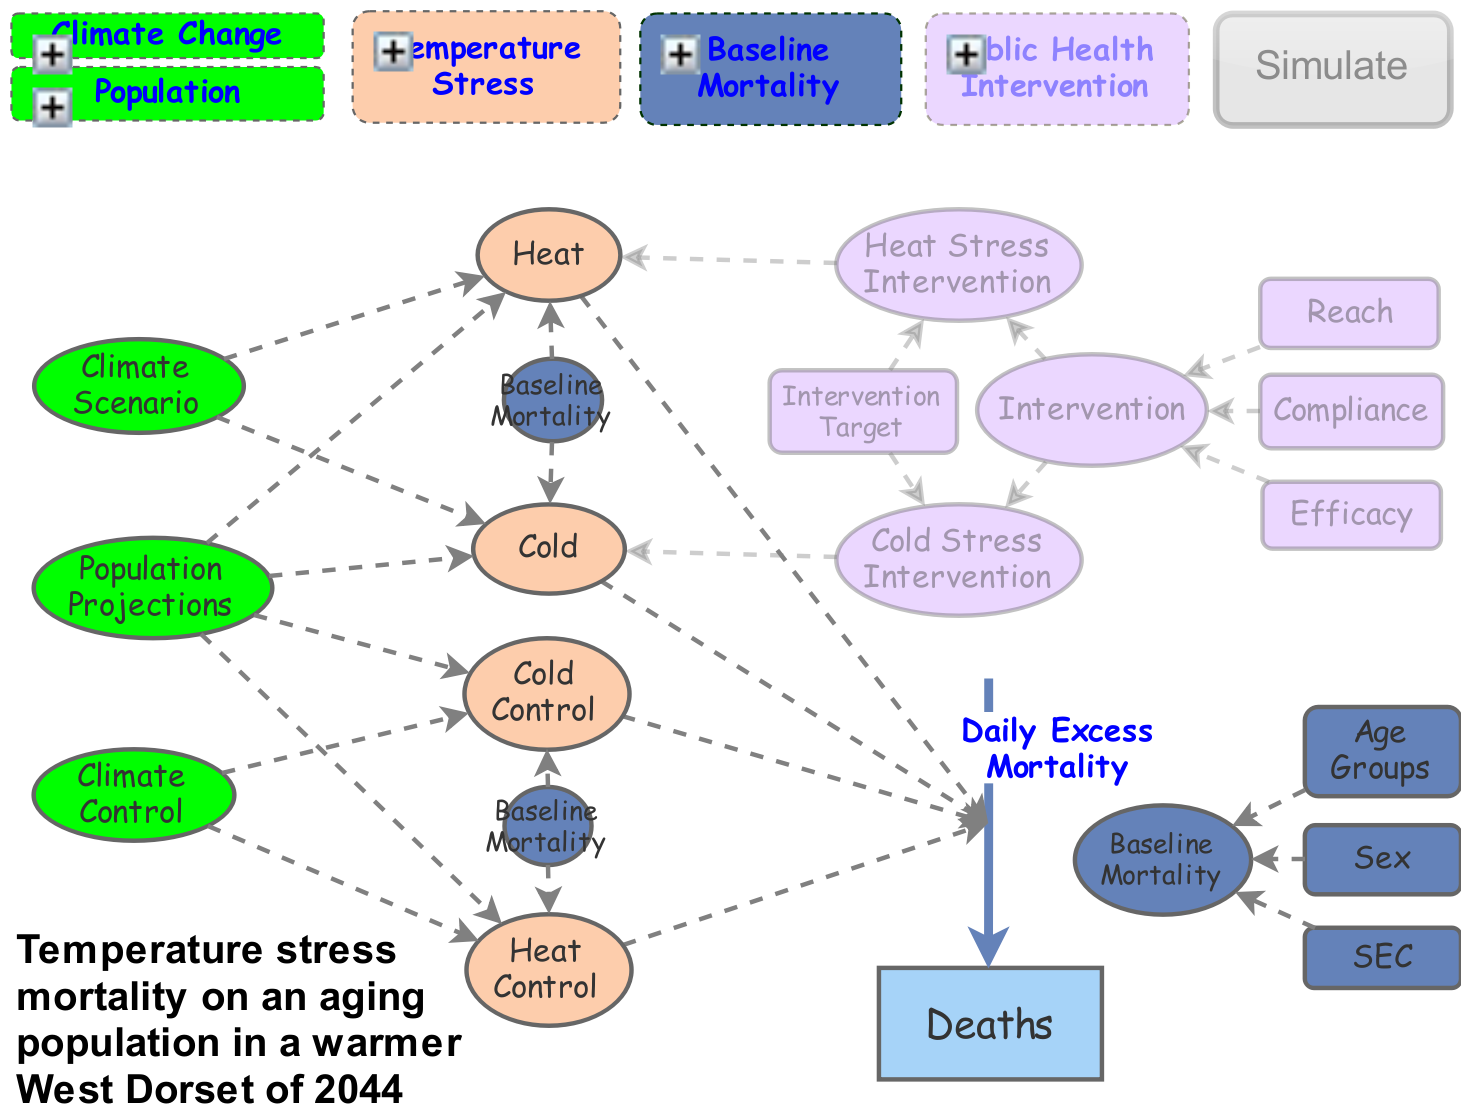
\includegraphics{./CCA/img/image_13.png}
	\caption[Cold Stress Excess Mortality is Higher]{It is worth noting at this point that even in a warmer West Dorset of 2044, mortality from cold stress will still be much higher than mortality from heat stress. Counter intuitive perhaps, but true. Of course excess mortality due to cold stress will be lower in the future (although still much higher than heat stress). More on this later -- it has implications for public health interventions. There are four `daily excess mortality' values estimated: excess mortality from future heat and cold stress and for comparison `control excess mortalities' are also estimated.}
\end{figure}

\begin{figure}[htbp]
	\centering
	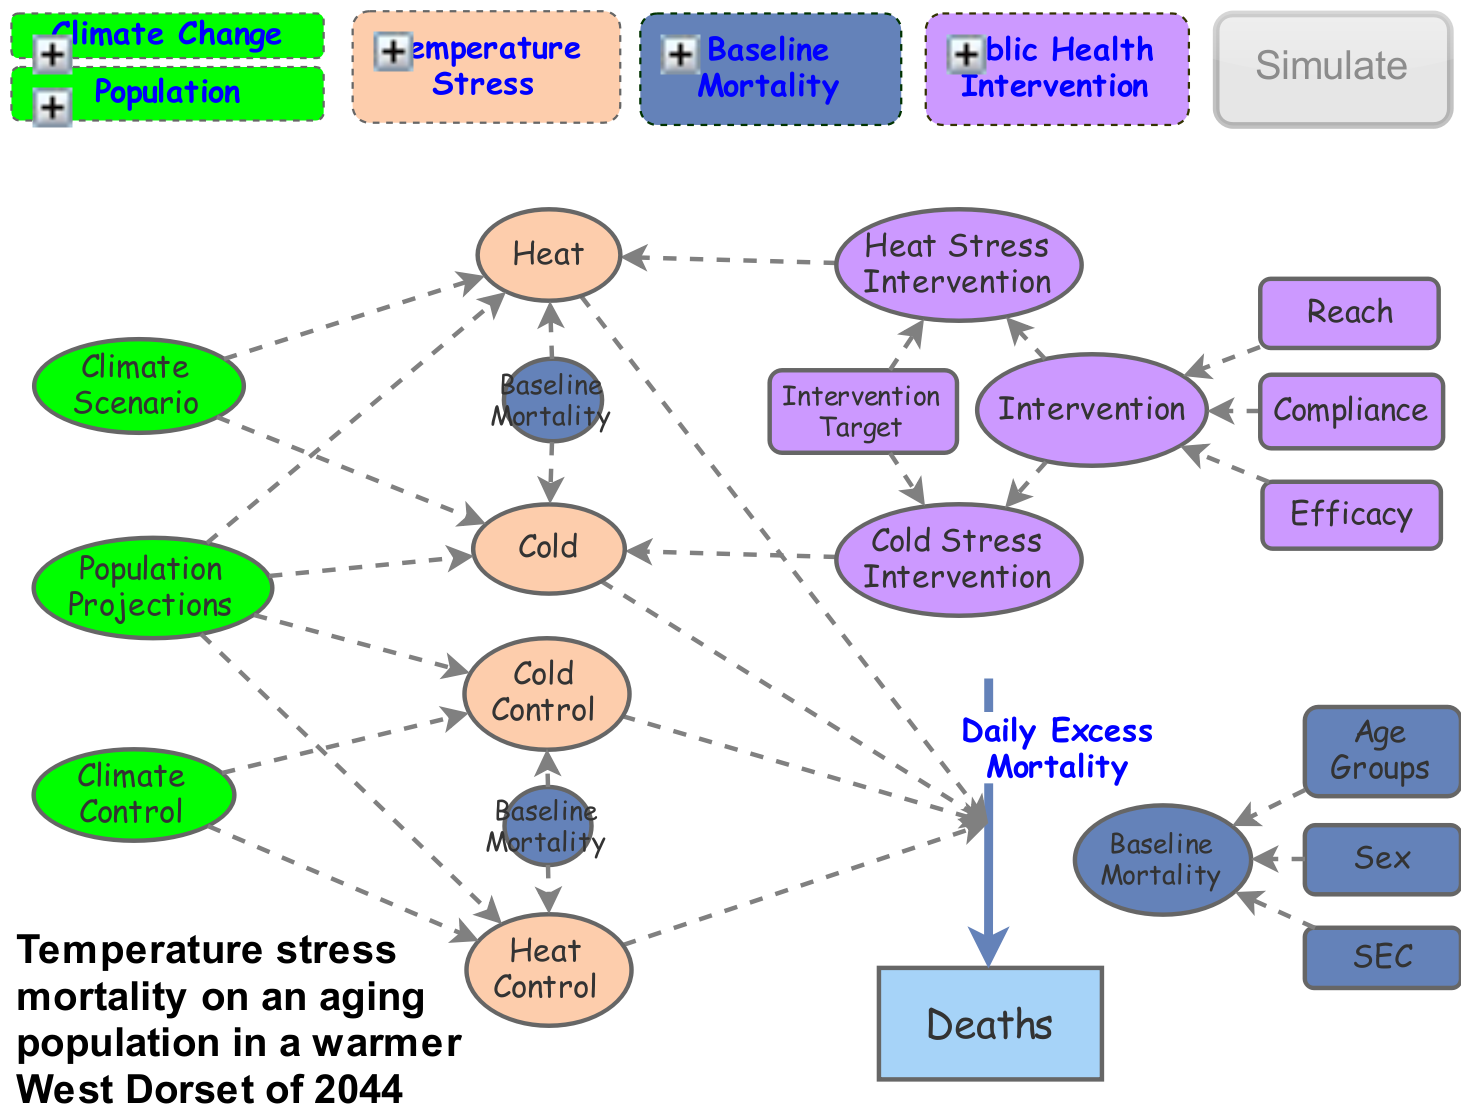
\includegraphics{./CCA/img/image_14.png}
	\caption[Devising Public Health Interventions]{You can compare these sources of excess mortality as they accumulate over the simulation period.So what public health interventions might be taken in order to assist the target population in adapting to more heat stress?}
\end{figure}

\begin{figure}[htbp]
	\centering
	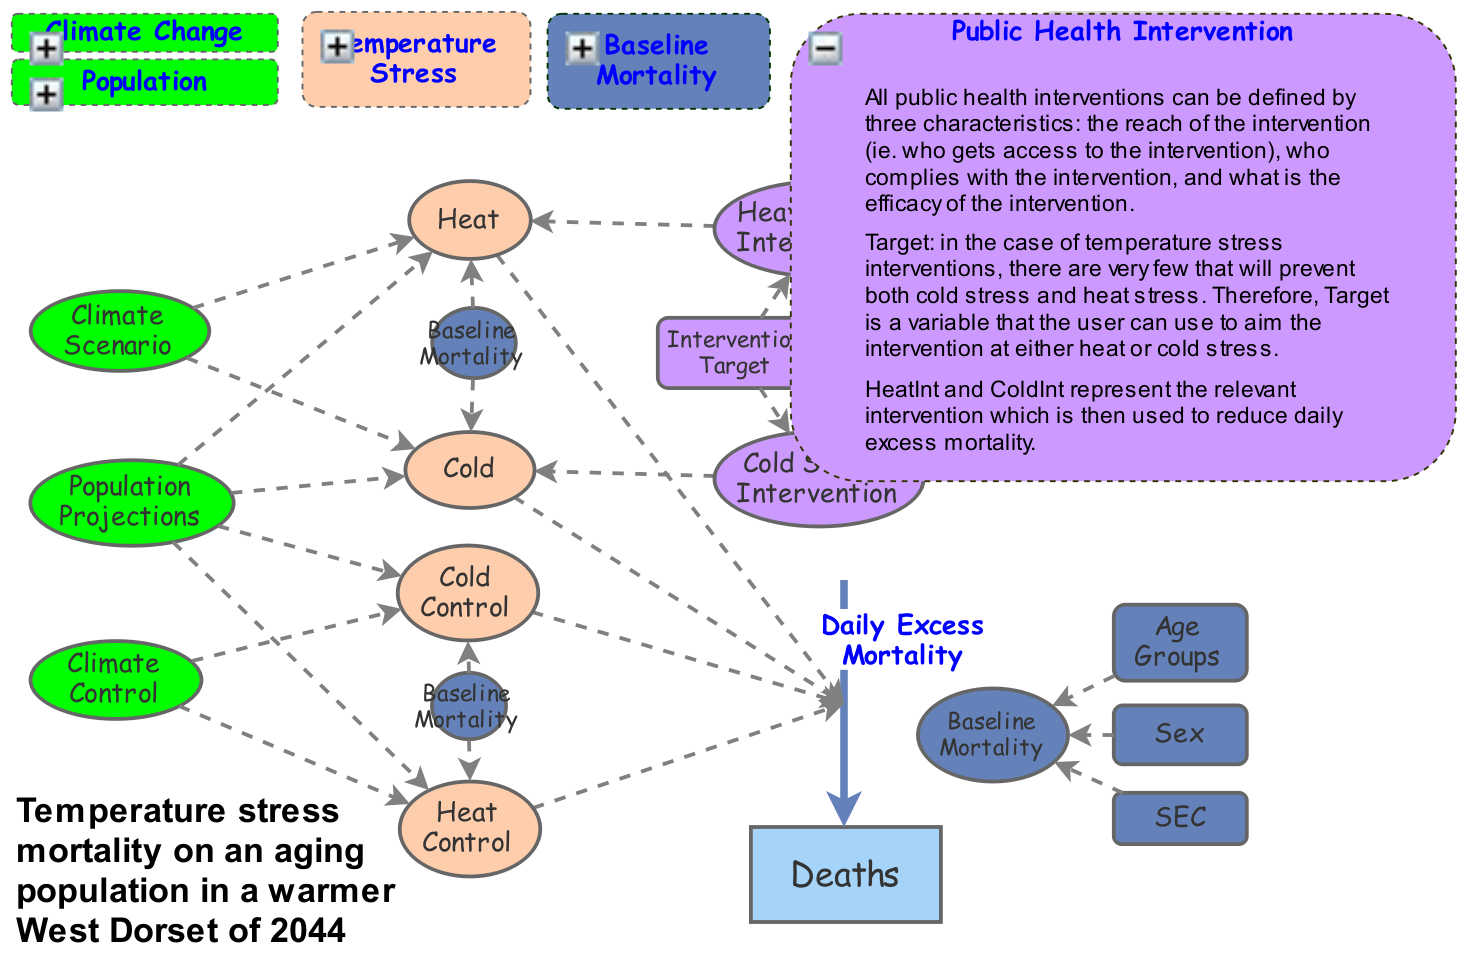
\includegraphics{./CCA/img/image_15.png}
	\caption[Intervention Targeting Options]{You have the option of trialling an intervention for either heat or cold stress, but not both at the same time. The default setting is for NO intervention. `Intervention Targeting' is the variable used to set which intervention will be made.}
\end{figure}

\begin{figure}[htbp]
	\centering
	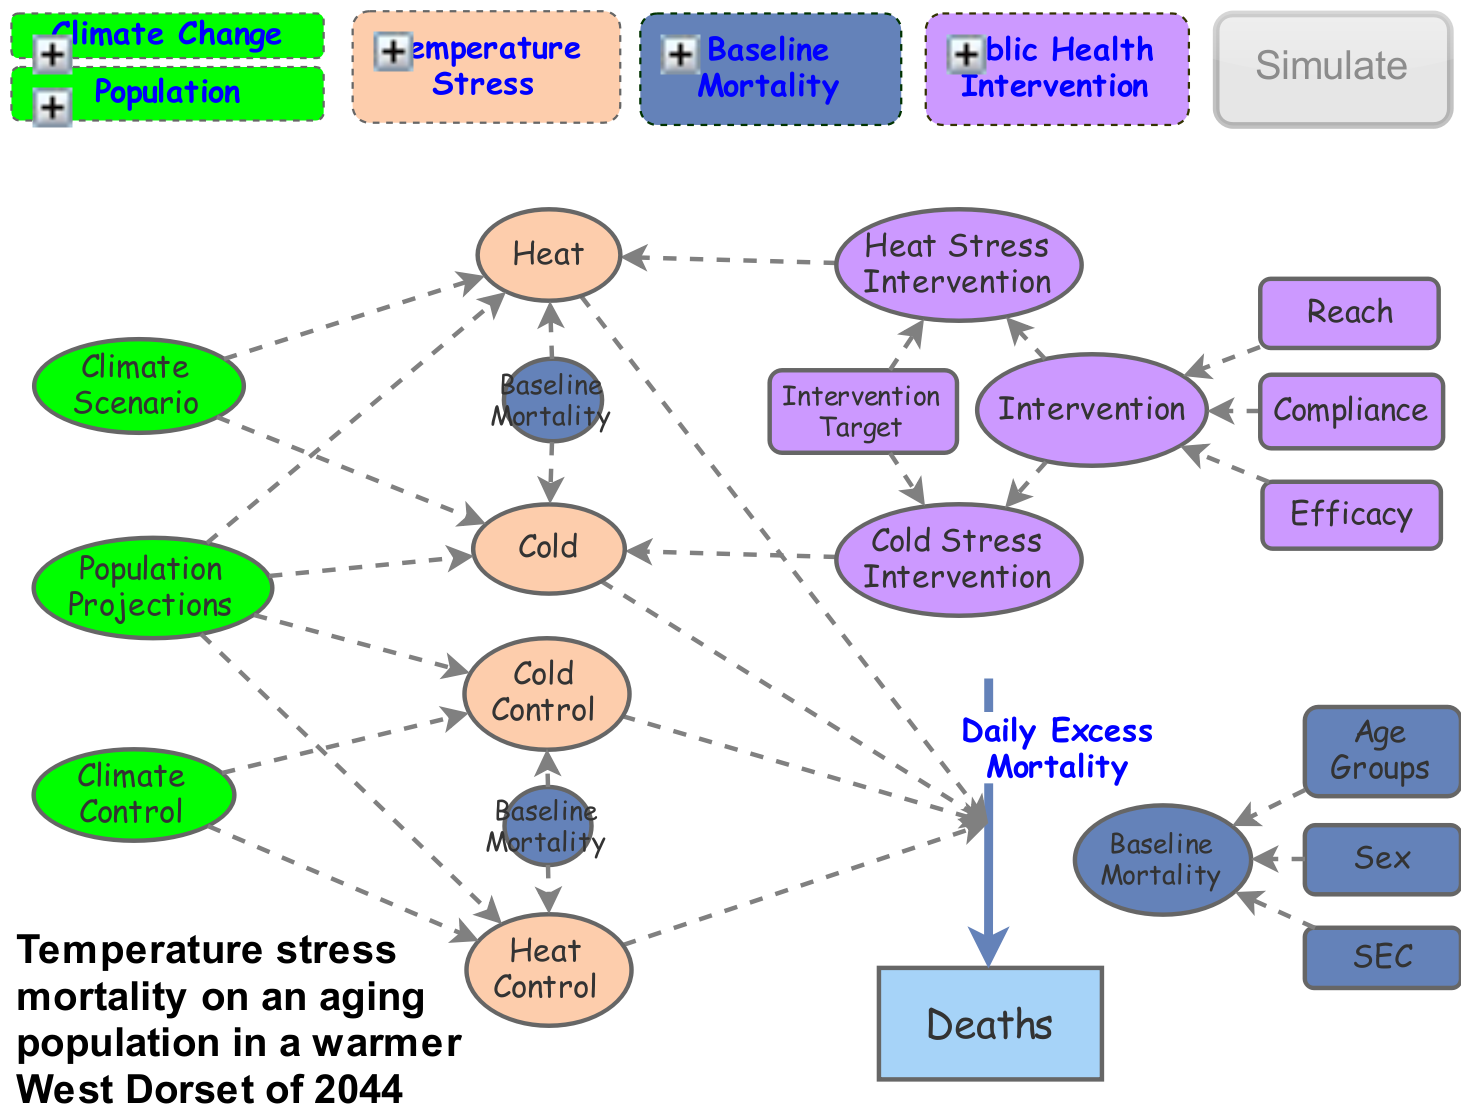
\includegraphics{./CCA/img/image_16.png}
	\caption[Elements of a Public Health Intervention]{All public health interventions have three basic variables: the proportion of the target population you can reach, the proportion of the population that comply with the intervention and the efficacy (how effective it is at doing what it is supposed to do) of the intervention.}
\end{figure}

\begin{figure}[htbp]
	\centering
	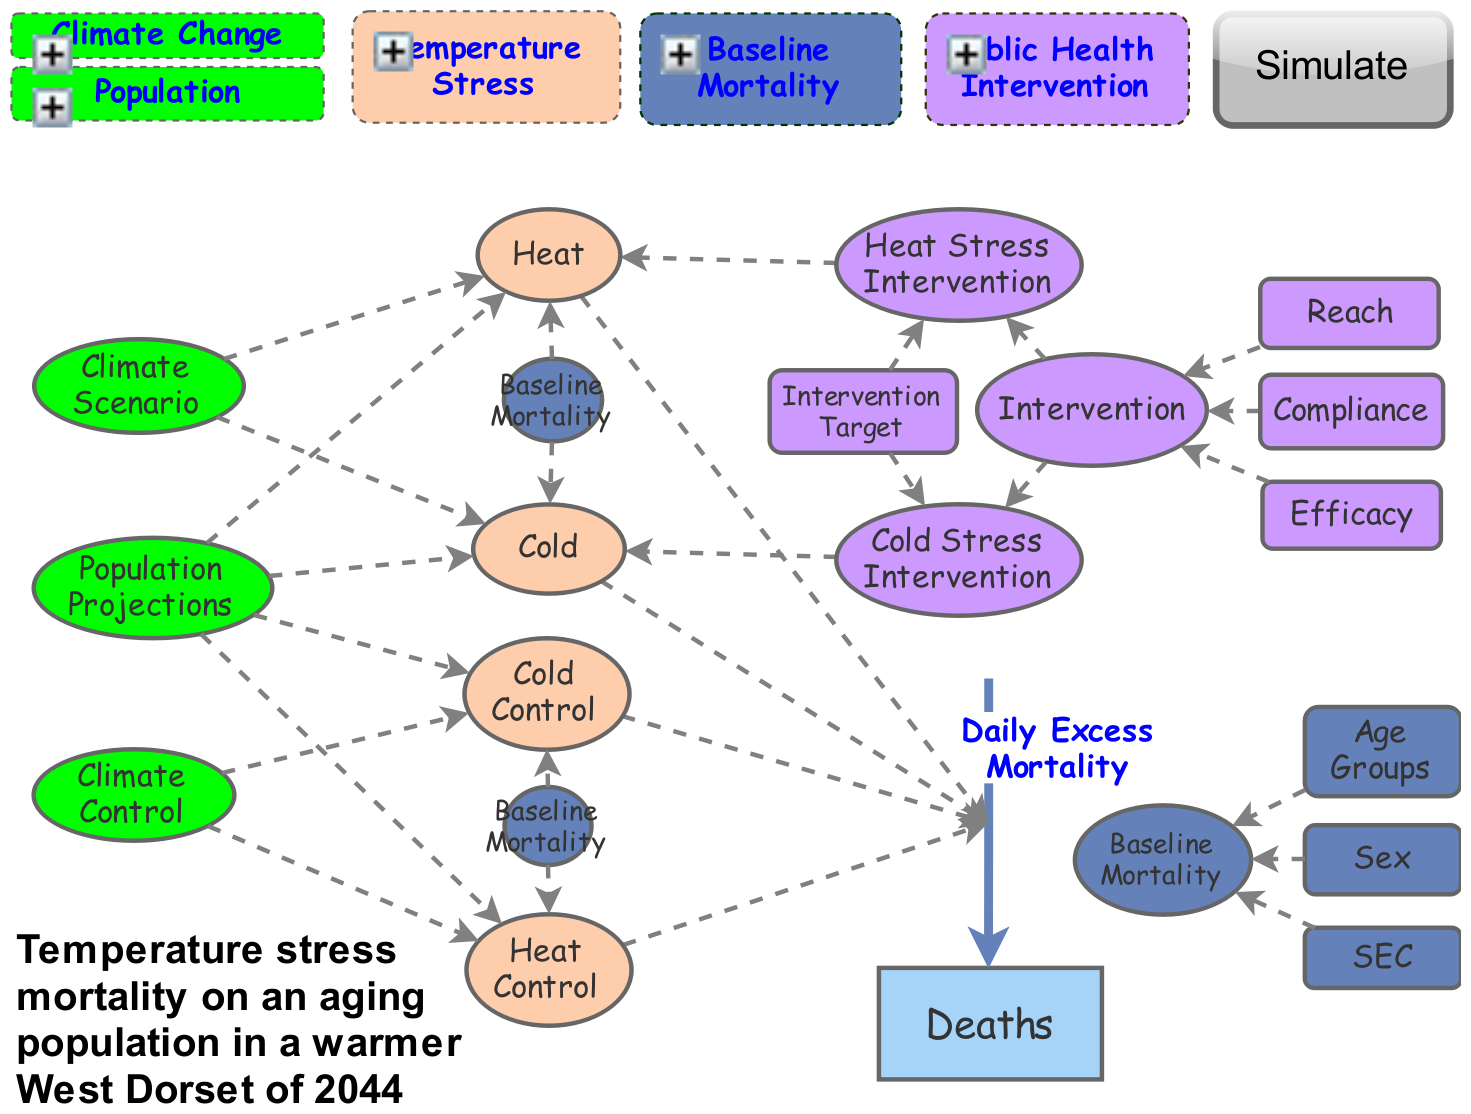
\includegraphics{./CCA/img/image_17.png}
	\caption[Run Simulation]{This `simulate' button produces the default simulation for a population with all age groups, all socio-economic classes and all both sexes included as a single population. Additionally, there are 10 years of simulated temperature data available (this default simulation setting uses the first 365 days). However, the `Settings' button at the top of the window allows the user to set the start and duration of the simulation period. The user will be presented with two daily excess mortality graphs (one for the future and one for the control), a combined accumulated deaths (both future and control) and a table of accumulated deaths.}
\end{figure}

\begin{figure}[htbp]
	\centering
	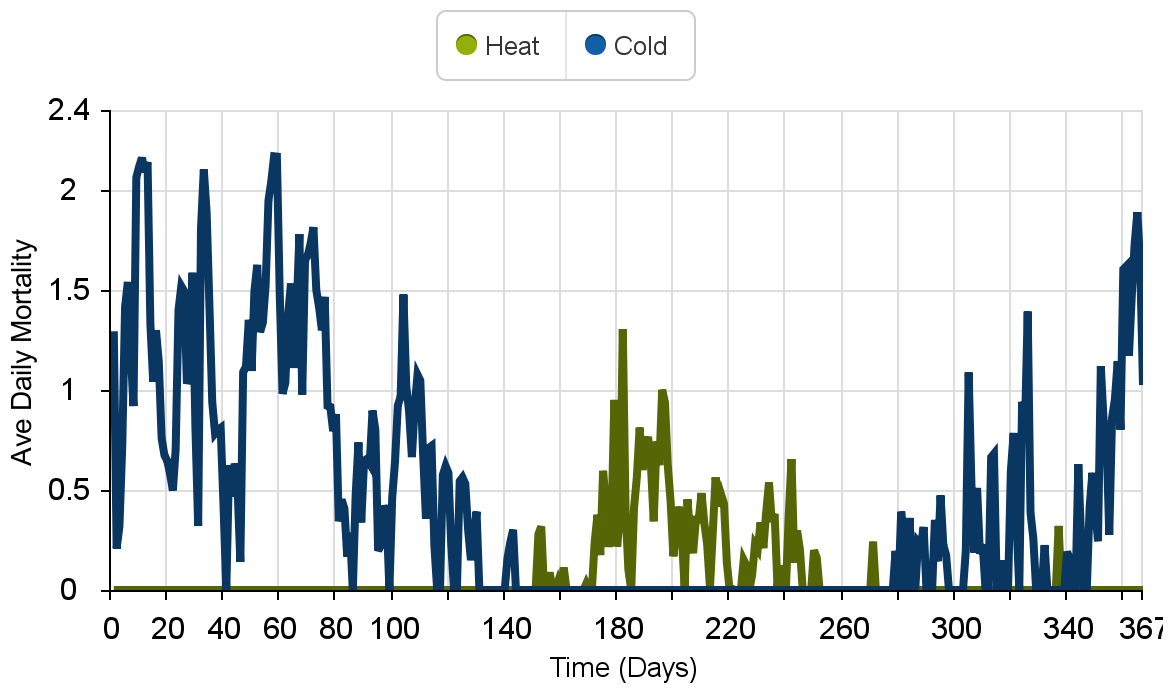
\includegraphics{./CCA/img/image_18.png}
	\caption[Simulation Output]{Do you see the three graph `tabs' above the graph? You can move between the visuals during the simulation. You can change the speed of the simulation and rerun it. The introduction to this model is now complete. You can `Exit Story' (bottom left of screen) and explore the model, its variables and its construction at your own pace. If you are unfamiliar with the Insight Maker modelling environment, you may wish to further explore that -- all models are open source -- set up your own free account to copy and modify this or any model for your own use and share with colleagues.}
\end{figure}



% Section 3 Futures Thinking
\section{Applications of Futures Thinking}
\label{horizonscanning}

\subsection{Introduction}
Futures thinking is...

This is a section to introduce futures thinking as a subtopic of systems thinking

Also called foresight

\subsection{Horizon Scanning}
Although, horizon scanning\cite{WikipediaFT} was essential to the development of future scenarios and the writing of a futures story, it was not made accessible outside of the project team and participants in our workshops. There were a couple reasons for this, the first was that we had very limited scope within the project to engage with the public and therefore limited our engagement to the futures story and secondly, the format produced by the horizon scanning tools was fairly rough and would be a lot of work to devise a method of communicating this directly.


During 2014, active horizon scanning was undertaken using the \url{http://www.shapingtomorrow.com/} web site. Membership is free and the site has numerous tools to enable future studies.

\begin{marginfigure}
	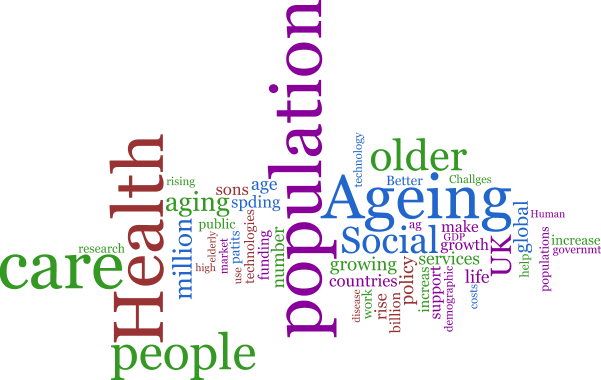
\includegraphics{CCA/img/FutureOlderPersonsWordCloud.png}
	\caption{Word cloud visualisation of horizon scanning results}
	\label{fig:wc}
\end{marginfigure}

What follows are the automatically derived insights generated by the Shaping Tomorrow tools from articles that were collected and run through their process. These tools are still in development and some of the automatically generated text is formatted poorly and/or grammatically incorrect due to the method used to extract the text (Figures~\ref{fig:wc}~and~\ref{fig:imap}).

\begin{figure*}
	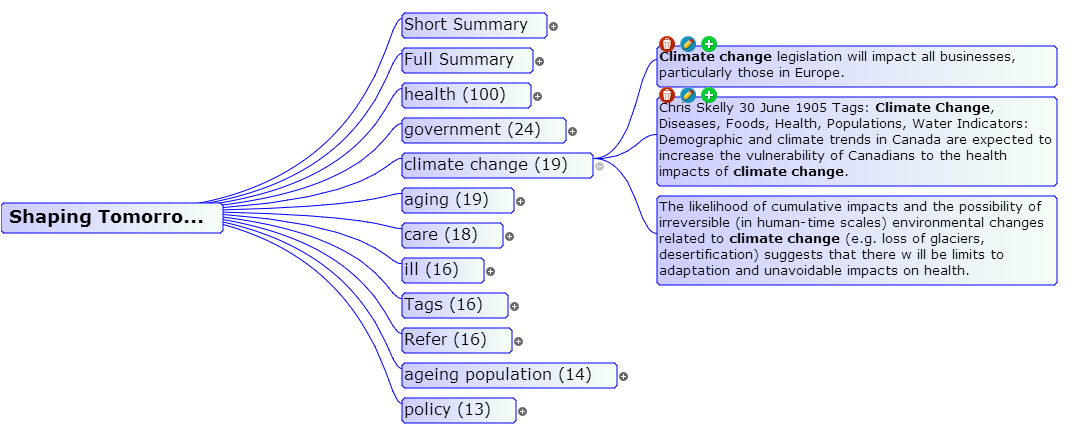
\includegraphics{CCA/img/WebSummarizerClimatechange.png}
	\caption[Shaping Tomorrow Tools]{A number of tools within Shaping Tomorrow's horizon scanning provide visual mapping of the results.}
	\label{fig:imap}
\end{figure*}

\begin{itemize}
	\item A lack of large-scale societal support programs for older populations in some Asian countries will be a major challenge for governments.
	\begin{quotation}
		Reflecting long-held ideas of functional foods derived from traditional medicines, Asia is the leading market for nutraceuticals.126 ? In 2010, China became the world's largest nutraceutical market.127 Implications and opportunities to 2040 The ageing of East Asia will happen much more rapidly than the ageing of the US and Europe; hence, East Asia will be forced to adapt more rapidly. A lack of large-scale societal support programs for older populations in some Asian countries will be a major challenge for governments.
	\end{quotation}
	\item Retraining and continuous learning will be at a premium and retirement policy will change dynamically.
	\begin{quotation}
		Climate change legislation will impact all businesses, particularly those in Europe. Energy and debt will remain important influencers of government policy for the coming decade. With less new foreign talent and more older workers, retraining and continuous learning will be at a premium and retirement policy will change dynamically.
	\end{quotation}
	\item Losing the smartest talent to more attractive economies will hamper R\&D and innovation.
	\begin{quotation}
		Consumers and employees are becoming older and more ethnically diverse in many European markets. Increasing productivity in ageing markets is essential if their economies are to avoid protracted difficulties. Losing the smartest talent to more attractive economies will hamper R\&D and innovation.
	\end{quotation}
	\item Ageing will affect almost every global economy in the coming years.
	\begin{quotation}The share of older people in the total population will increase significantly in the coming decades, as a greater proportion of the post-war baby-boom generation reaches retirement. This will, in turn, lead to an increased burden on those of working age to support the social expenditure required by the ageing population for a range of related services36. Profound in its implications for pension schemes, taxation, business talent, economic competitiveness not to mention health and service provision, ageing will affect almost every global economy in the coming years.\end{quotation}
	\item Consistently low birth rates and higher life expectancy will transform the shape of the EU27's age pyramid.
	\begin{quotation}Steria: The Future Report 2012 \url{www.steria.com}{www.steria.com} Ageing populations The impact of demographic ageing within the EU is likely to be of major significance in the coming decades. Consistently low birth rates and higher life expectancy will transform the shape of the EU27's age pyramid, probably the most important change will be the marked transition towards a much older population structure and this is already becoming apparent in several Member States.\end{quotation}
	\item Expect there to be less loyalty to the organisation.
	\begin{quotation}
		The next decade of change for organisations and workers Effects of change on workers Over the coming decade, survey respondents expect employees to work longer hours, retire at an older age, and experience greater personal and family stress due to work. Given that outlook, it is unsurprising that 57\% of respondents expect there to be less loyalty to the organisation\dots\end{quotation}
	\item Expect employees to work longer hours.
	\begin{quotation}
		Believes global collaboration lets GM leverage scarce human resources and innovate more quickly, while its regional engineering centres allow it to leverage knowledge of markets. The next decade of change for organisations and workers Effects of change on workers Over the coming decade, survey respondents expect employees to work longer hours, retire at an older age\ldots\end{quotation}
	\item Human Health  in a Changing Climate: Canadian Assessment of Change
	\begin{quotation}
		Climate Change Adaptation and Health Equity: Social and health care planning for older persons must consider the social, psychological and physical dimensions of their lives\end{quotation}
	\item Age discrimination in the provision of surgery will become an increasingly big problem for older persons
	\item PCTs have come and gone -- but the same issues remain
	\item Health and social care spending - no solution in sight - only increased budget pressure
	\item Polypharmacy and medicines optimisation required to control costs of health care for older persons.
	\item Complexity of multiple chronic conditions in older persons driving `health care integration'
	\item The future of sustainable health and social care will depend upon volunteers	
	\item Key concerns for climate change adaptation in the UK include inequality, rurality and an ageing population
	\item The UK population is ageing - can we change our systems and funding before we are in crises?
	\item Ageing: opportunity or challenge?
	\item The nature of primary care in the UK must and will change
	\item Hospitals and health system moving to a patient centred paradigm
	\item The role of hospitals and doctors will change
	\item Future of the health service: the era of community care has arrived
	\item The focus on quality of life issues for future older persons will change everything
	\item Rethinking the funding model for social and health care for older Britons
	\item Social care system for older persons in the UK is not fit for purpose and needs to be redesigned
	\item Fuel poverty still not being addressed in local authority planning across the UK
	\item Public policy to improve the lives of Older persons in UK needs to continue to evolve
	\item Ageing policy in 2013/14 - curate's egg or turning point?
	\item The Tip of the Iceberg
	\item Consumer technologies for assisted living are increasingly being designed for an ageing population
	\item Increasing dementia set to dominate social and health care services for older persons
	\item The rise of the 4th Generation -- the needs of the 85+ crowd are not the same as the younger olds
	\item State Pensioner poverty is projected to decrease to 10\% by 2025
	\item Increased funding demands on social services for Older Persons in UK is changing the funding model
	\item Despite the growing population of Older Persons support funding is set to decline
	\item Social isolation is an increasing problem amongst older persons
	\item The nature of support services for independent living for older persons with frailty will change
	\item Care Bill [HL] - Commons Library Research Paper
	\item Fuller working lives: a framework for action
	\item Private benefits of participation in higher education will likely remain high due to increasing relative demand for skilled labour.
	\begin{quotation}
		The case for government support for life-long learning may in fact be stronger here than for tertiary education for the young, as lower cross-country mobility among older workers means that the social benefits in terms of higher productivity and longer careers to a larger extent will benefit the domestic economy. Fiscal constraints and international mobility of skilled labour will make co-payments for higher education more attractive 55. Private benefits of participation in higher education will likely remain high due to increasing relative demand for skilled labour.\end{quotation}
	\item Fiscal constraints and international mobility of skilled labour will make co-payments for higher education more attractive.
	\begin{quotation}
		While longer working lives will increase incentives to invest in education, it will also raise risks that acquired education and skills become obsolete, requiring an increased emphasis on life-long learning. The case for government support for life-long learning may in fact be stronger here than for tertiary education for the young, as lower cross-country mobility among older workers means that\dots\end{quotation}
	\item For elderly people the development and production of bespoke products tailored to individual needs will particularly benefit from the design freedom and flexibility that Digital Fabrication offers.
	\begin{quotation}
		Society: Consumer requests for personalised, comfortable, safe, healthy, affordable and sustainable products are growing over a range of sectors from high technology goods to apparel, footwear and household products. Technology solutions will also need to be developed to respond to the challenges posed by an ageing population. For elderly people the development and production of bespoke products tailored to individual needs will particularly benefit from the design freedom and flexibility that Digital Fabrication offers.\end{quotation}
	\item Government departments and third parties will need to work together to meet rising demands for integrated delivery in human and social services such as income security, employment assistance, social housing, aged care and child welfare.
	\begin{quotation}
		Meaningful collaboration with citizens, other levels of government, neighboring regions and the private and non-profit sectors is essential to mobilizing the necessary knowledge, capital and resources required to sustain key areas of government service delivery. For example, various government departments and third parties will need to work together to meet rising demands for integrated delivery\ldots\end{quotation}
	\item Cold Weather Plan  for England 2013
	\item Fears raised 'free NHS' will come to an end
	\item Workers in older age groups will need to embrace technology fully in order to compete in the labour market.
	\begin{quotation}
		Cross-generational skills acquisition will be important. While the speed of technological change may place younger cohorts at a perceived advantage, especially those who have grown up entirely in a digital age, all age cohorts will need to invest in continual up-skilling to keep pace with accelerating development. Workers in older age groups will need to embrace technology fully in order to compete in the labour market.\end{quotation}
	\item 2014 Global life sciences outlook - Resilience and reinvention in a changing marketplace
	\item Social networks will help to determine where and how people will want to live.
	\begin{quotation}
		We think these trends are likely to alter real estate economics more than is currently anticipated. Beyond 2020, the generation that has grown up in the digital world will dominate consumer spending and the culture of work. Social networks will help to determine where and how people will want to live, work and recreate.\end{quotation}
	\item Baby Boomers will work longer.
	\begin{quotation}
		Why the Retirement Age Must Go Up. It notes that North America has a ``smidgeon'' more room than European countries, allowing for slightly earlier retirement. However, the message is stark: Baby Boomers will work longer, adding new pressures to labor markets that are recovering slowly from the aftermath of the Great Recession.\end{quotation}
	\item Generation Y members will make up about 50 per cent of the working population in the UK (ONS, 2011a).
	\begin{quotation}
		Currently, 12 million people over the age of 18 fall into the Generation Y age range in the UK (ONS, 2011a). 67 Potential future developments By 2030, Generation Y members will make up about 50 per cent of the working population in the UK (ONS, 2011a), dominating the talent pool.\end{quotation}
	\item Health and Health Care in 2032
	\item The Future of Healthcare  in Europe
	\item Policy makers will need to consider indirect as well as direct implications of policy for communities and people's sense of belonging.
	\begin{quotation}
		However, hyper-connectivity can also create or strengthen new group identities. Policy makers will need to consider indirect as well as direct implications of policy for communities and people's sense of belonging. It is important to recognise that policies can interact with identities in complex and unpredictable ways.\end{quotation}
	\item The `pensioners of tomorrow' will be digitally savvy -- 54\% of adults aged 54 to 65 now own a smartphone.
	\begin{quotation}
		12.6 million in England volunteer at least monthly. The proportion of older people who come from a minority or ethnic background is expected to more than double by 2033. 66\% of charity trustees in England and Wales are aged 50 and over.\end{quotation}
	\item Revenue likely will drop to 15\% inpatient/ 85\% outpatient.
	\begin{quotation}
		VP, Real Estate: Today, revenue is split 50\% inpatient/50\% outpatient. In the future, revenue likely will drop to 15\% inpatient/ 85\% outpatient. VP, Real Estate: There's an interesting transition happening: things that used to be in the hospital are moving into outpatient clinics and things that were in the outpatient clinics are moving to the home environment.\end{quotation}
	\item By 2050 almost every car and van in the UK will be an ultra low emission vehicle (ULEV).
	\begin{quotation}
		The UK Government is committed to grasping this opportunity. Our vision is that by 2050 almost every car and van in the UK will be an ultra low emission vehicle (ULEV), with the UK at the forefront of their design, development and manufacture, making us one of the most attractive locations for ULEV-related inward investment in the world. Context - the inevitable transition 3.\end{quotation}
	\item Standard population projections show that virtually all global growth over the next 30 years will be in urban areas.
	\begin{quotation}
		Understandably so: well over half of the world's population lives in cities, generating more than 80\% of global GDP. Standard population projections show that virtually all global growth over the next 30 years will be in urban areas. The number of people living in the world's cities is growing by nearly 60m every year.\end{quotation}
	\item Individuals aged 55 or older will account for 20\% of world population (or 1.6 billion out of 8 billion) in 2025.	
	\begin{quotation}
		In addition, the total number of megacities - with more than 10 million inhabitants - is projected to increase from 23 in 2011 to 37 by 2025 (see Figure 3), with nine new megacities emerging in Asia alone.10 Another development to consider is Global Ageing. Individuals aged 55 or older will account for 20\% of world population (or 1.6 billion out of 8 billion) in 2025. This ``silver segment'' is even expected to reach 35\% in G7 countries by 2025, a situation that will call for age-appropriate mobility solutions.\end{quotation}
	\item 2025: a very different world: are you ready?
	\begin{quotation}
		2025 is just over a decade away, and the scale of changes that are approaching are likely to make that decade tumultuous, for good and ill. Governments, organisations and individuals will all need to change their ways and learn new approaches if we are to take advantage of the positive and reduce the negative impacts.\end{quotation}
	\item Human enhancement and the future of work
	\item Future Hospital: Caring for medical patients
	\item Scientists in Australia make cochlear implants even better
	\item 2030 vision - the best and worst futures for older people
	\item Health and wellness - a `biggie'
	\item Ageing population pushes welfare bill to crisis point
	\item Ageing population has great potential
	\item Pill could help humans live longer
	\item Our Future World: Global megatrends that will change the way we live
	\item Challenges Of An Ageing Asia
	\item Japan turns to robots as population declines
	\item An elderly crisis and a youth crisis: South Korea's got it all
	\item Japan's ageing population: From silver to gold
	\item China Health-Care Spending May Hit \$1 Trillion by 2020
	\item Nursing care and robots
	\item Start-up capitalises on Japan's ageing population
	\item Nurses battling their own medical crisis
	\item Older workforces make commercial sense
	\item Countries With The Most People Over 100
	\item The cost of our ageing society
	\item Many to many: How the relational state will transform public services
	\item Games that are good for you
	\begin{quotation}
		Wellbeing and fitness gaming may soon go the way of health apps: grow fast. Health apps for smart phones appear in their 1000s in Apple and Android app stores and now Nintendo and Kinect are both chasing the gaming health and wellbeing dollar. But the games may appear not only in the living room: increasingly they may provide support for healthcare professionals in different contexts\end{quotation}
	\item China Elder Care Market Trends \& 2017 Forecasts
	\item 2030 vision for palliative and end of life care
	\item By 2040 you will be able to upload your brain\ldots
	\item Ageing Successfully Reversed in Mice; Human Trials to Begin Next
	\item Global cities and ageing
	\item Obesity pandemic looms large as half of Britons could be overweight by 2050
	\item Tiny Homes Can Serve Diverse Housing Needs
	\item How wearable tech may keep you alive a little longer
	\item 20 Predictions in Medicine And Healthcare for 2014: From DIY Biotech to Mind-Controlled Exoskeletons
	\item Electricity use drops as UK passes `peak light bulb'
	\item Turning off the `ageing genes'
	\item Tablets and apps might be doctor's orders of the future
	\item Anti-ageing formula slated to begin human trials
	\item Life Begins at 90 as Nonagenarians Show Sharp Brainpower
	\item A New?and Reversible?Cause of Ageing
	\item High BP pill could ease arthritis pain
	\item Skin's own cells offer new hope for skin repair
	\item Vancouver's ban on the humble doorknob likely to be a trendsetter
	\item Asia?s New Ageing Rich Break Family Ties for Gilded Retirement
	\item Salim Ismail: Top 5 Revolutionary Medical Breakthroughs by 2020
	\item Ageing Research at Yale: Past Present and Future
	\item The recent demographic, epidemiological and social trends in UK
	\item Fountain of youth? Scientists discover why wounds heal quicker for young people
	\item The changing shape of retirement funding in a greying ASEAN
	\item Google wants you to live 170 years
	\item The changing shape of retirement funding in a greying ASEAN
	\item Study: slowing ageing will give more financial, health gains than disease research
	\item Is the incidence of dementia declining?
	\item Global study: World not ready for ageing population
	\item Oncologists call for industry-led global fund to fight cancer
	\item The Future of Longevity
	\item Epigenetic markers shows promise in Alzheimer's disease
	\item Global study: World not ready for ageing population
	\item Life expectancy gap growing between rich/poor world women: WHO
	\item Immune to ageing
	\begin{quotation}
		While ageing remains an inevitable fact of life, Max Planck researchers have discovered a microbe that stays forever young by rejuvenating every time it reproduces\end{quotation}
	\item What can we do to make cities less lonely for the elderly?
	\begin{quotation}
		A series of commentaries and tagged photos illustrate key points: many global cities target the young - not ideal in ageing societies; immigrant families often live multi-generationally - new designs are needed; `golf carts' could provide increased mobility everywhere; multi purpose facilities that focus on older people but include all; and good business sense targeting older consumers.\end{quotation}
	\item New method prevents muscle loss
	\begin{quotation}
		New Australian research suggests that a small dose of testosterone directed solely to the liver stimulates protein synthesis, likely preventing muscle loss and wasting, and potentially promoting muscle growth\end{quotation}
	\item For Gesture Control, a Startup Wants to Feel Your Muscles
	\begin{quotation}
		The  Myo armband interprets the electrical impulses of muscle movements in your forearm, does not need light or a camera to operate and can tell the difference between different finger movements, sense hand rotations and movements by measuring the different electrical-impulse patterns.\end{quotation}
	\item Japan looks to new technology to cater for ageing population
	\begin{quotation}
		The Japanese government is encouraging more companies and universities to develop robots to care for the elderly population.\end{quotation}
	\item The Next Big Infrastructure Crisis? Age-Proofing Our Streets
	\begin{quotation}
		Age friendly cities need investment in all sorts of infrastructures from longer crossing times to more street shelters and seats. Agelab from MIT helps designers understand the effects of ageing. Walkable communities will be critical.\end{quotation}
	\item Why Older Minds Make Better Decisions
	\begin{quotation}
		Scientists are discovering that even though memory skills decline with age, the choices we make may improve\end{quotation}
	\item Boosting `cellular garbage disposal' can delay the ageing process, UCLA biologists report
	\begin{quotation}
		UCLA life scientists have identified a gene previously implicated in Parkinson's disease that can delay the onset of ageing and extend the healthy life span of fruit flies. The research, they say, could have important implications for ageing and disease in humans\end{quotation}
	\item Scientists discover how to slow down ageing in mice and increase longevity
	\begin{quotation}
		Scientists have found that the hypothalamus of mice controls ageing throughout the body\end{quotation}
	\item 8 Exponential trends that will shape humanity
	\begin{quotation}
		80\% of what doctors do today will be replaced by technology in 10 years time. With the rise of digital health, increasing numbers of apps and sensors, more people are taking their health into their own hands.\end{quotation}
	\item Scientists find key to ageing process in hypothalamus
	\begin{quotation}
		The US team identified the mechanism in the hypothalamus, which sits deep inside the brain, and showed they could tweak it to shorten or lengthen the lives of animals.\end{quotation}
	\item EFP Policy Workshop: Smart Mobility 2050 -- Human centred Vision and long-term Horizon \textregistered European Foresight Platform
	\begin{quotation}
		Transport and mobility can no longer grow at the same pace without serious environmental, social and economic consequences. 4 visions of mobility in 2050 and the full workshop discussion paper. Need for policies to support more fluid, greener, safer accessible transport.  \url{http://www.foresight-platform.eu/wp-content/uploads/2012/03/EFP-Smart-Mobility-Workshop-Paper.pdf}\end{quotation}
	\item EFP European Policy Workshop on Active and Healthy Ageing a long term View \textregistered European Foresight Platform
	\begin{quotation}
		Presentations and documentation from a workshop on active and healthy ageing.  Innovations that are useful, policy responses under way. Full report here: \url{http://www.foresight-platform.eu/wp-content/uploads/2011/03/Paper\_Active\_Healthy\_Ageing\_ML\_FIN.pdf}\end{quotation}
	\item Wearable technology - from geek to chic?
	\begin{quotation}
		Wearable technology: smart watches and smart glasses especially, but others too are being touted as the next big thing. And the race is well and truly on with giants such as Apple and Google entering the field but also smaller companies such as Pebble and mc10. The challenge will be to overcome the geek image much wearable technology has had until now and make us ?want? another device. Specialist applications may indicate the way forward at first, especially in sport and health.\end{quotation}
	\item Plastic compound provides foundation for bone regeneration
	\begin{quotation}
		A plastic compound with sponge-like pores can replace damaged bone and allows the patient's own cells to grow into and take over the material.\end{quotation}
	\item iDoctor: Could a smartphone be the future of medicine?
	\begin{quotation}
		The apps available for smart phones could be a key to cheaper medical care, and diagnosis across a range of medical tests. In this video, some of the applications are shown in practice.\end{quotation}
	\item Ageing in the 21st Century
	\begin{quotation}
		The world is getting much older. Within 10 years, there will be 1 billion older people worldwide\end{quotation}
	\item Is Japan heading for a Zombie future?
	\begin{quotation}
		This century will witness the long, slow sunset of Japan's power\end{quotation}
	\item HR strategies for a multigenerational workforce
	\begin{quotation}
		HR strategies must deal with an ageing workforce that includes retaining ageing workers for longer, in addition to attracting and retaining younger workers.\end{quotation}
	\item Creating a future for Japan's ageing society
	\begin{quotation}By 2050, nearly 40 percent of Japan population will be 65 or over. . Nothing like these demographics has ever been seen before, here or anywhere.For 13 straight years, suicide has claimed more than 30,000 Japanese lives annually, carnage worthy of a civil war. This is not exclusively ? but is increasingly.\end{quotation}
	\item Specs and the city: planning for an ageing urban population
	\begin{quotation}With the ageing population, creating communities that meet their needs is now a major concern for social and public policy and involving them in the social and economic life of cities will be a crucial task for urban development. Keele University and Manchester are exploring a number of projects in support of age friendly cities.\end{quotation}
	\item Twenty percent of student loans are held by students over fifty
	\begin{quotation}20\% of student loans are actually held by Baby Boomers - and they account for fully 22\% of all defaults\end{quotation}
	\item Globalization, Ageing Challenge Growth
	\begin{quotation}Globalization and ageing are two sides of the same coin, says a noted author who has written extensively about socio-economic trends; as we age and chose to have smaller families, we increasingly rely on the affordable labor of foreign workers\end{quotation}
	\item United States sets 2025 goal to tame Alzheimer's
	\begin{quotation}The United States says it will seek an effective treatment for Alzheimer's by 2025.  The United States faces an ageing population and spiralling health costs.\end{quotation}
	\item Italy's `triangle of death' linked to premature ageing
	\begin{quotation}Illegal waste dumps in Italy may be causing nearby residents to age faster than they should\end{quotation}
	\item Self management for arthritis now
	\begin{quotation}A new self injecting version of Orencia, a previously intravenous drug treatment for RA, has been listed by the PBS.\end{quotation}
	\item The Disruptive Force that is Demography
	\begin{quotation}There are many trends we could consider as we look at the study of changing populations, but the most important ones that will impact business in the next 3 to 5 years are: an ageing population (and changes in retirement), rising life expectancy, plummeting fertility rates, the potential for generational conflict, migration and diversity\end{quotation}
	\item `Jam' with Health Horizons' Director Rod Falcon and Philips on the Future of Ageing Well
	\begin{quotation}How do we age well? It's a challenge each of us will face as individuals someday, if we're not doing so already. But all over the globe, we're seeing average population age increase, and, in the future, we'll have to address this shift collectively\end{quotation}
	\item Multiple medicine use very common: new snapshot of over-50's medicine habits
	\begin{quotation}A study has provided new insights into how people use medicines on a daily basis and highlights that the use of multiple medicines in older Australians is common and more complex than previously thought. Key findings: most commonly taken active ingredients were omega-3 fatty acids (fish oil), paracetamol, aspirin and glucosamine\end{quotation}
	\item A new vision for old age
	\begin{quotation}The good news is that Europe is ageing. In a little over half a century, the average life expectancy has gone from 66 to 75, and by 2050 is predicted to hit 82. This is not simply because people are not dying young, but because they are living to older ages than ever: the over 85s are the fastest growing demographic group on the continent\end{quotation}
	\item Rising to the challenge of peak population
	\begin{quotation}
		In 2011, world population passed the 7 billion mark. While growth will continue, total fertility rates are falling fast and will result in slower population growth and possibly, according to some, declining total population. Lower fertility rates may bring a demographic dividend, significant opportunities but also challenges. Or, we may be doomed, as others would suggest.\end{quotation}
\end{itemize}


\subsection{Futures Story}

\subsection{Scenarios}
There are a number of futuring techniques available that allow for an exploration of possible future states.

\begin{quotation}
	Scenarios are one of the most popular and persuasive methods used in the Futures Studies. Government planners, corporate strategists and military analysts use them in order to aid decision-making. The term scenario was introduced into planning and decision-making by Herman Kahn in connection with military and strategic studies done by RAND in the 1950s.
	
	It can be defined as a rich and detailed portrait of a plausible future world, one sufficiently vivid that a planner can clearly see and comprehend the problems, challenges and opportunities that such an environment would present.
	
	A scenario is not a specific forecast of the future, but a plausible description of what might happen. Scenarios are like stories built around carefully constructed plots based on trends and events. They assist in selection of strategies, identification of possible futures, making people aware of uncertainties and opening up their imagination and initiating learning processes.
	
	One of the key strengths of the scenario process is its influence on the way of thinking of its participants. A mindset, in which the focus is placed on one possible future, is altered towards the balanced thinking about a number of possible alternative futures.\cite{WikipediaSP}
\end{quotation}

We used Systems Modelling, horizon scanning and a brainstorming workshop to identify trends and potential public health interventions. This allowed us to develop a scenario and communicate it using a `Futures Story'.

\subsection{Community Leader Will Be Missed} 
Obituary\sidenote{An unusual but common form of writing, chosen because many people in our target group of 50 years reads them.}

Susan Williams: Hugely popular and tireless community worker who was known for both a humane and common sense approach to life. The founder of the Nettlepuddle-Eco-Village and one of the most influential movements in elder care was to her amusement often publicly referred to as ``that woman who brought down the Prime Minister'' in 2030.\sidenote{Establish \emph{interest}, she was local AND important, and seed \emph{Futures themes}, eco, community, elder care.}

Chris Skelly

Saturday, 7 January 2045\sidenote{Establish future period of writing.}

A chance invite to participate in a live panel discussion on climate change adaptation in 2029, saw Susan Williams catapulted into the media spot light, much to her surprise and amusement. Replacing a last minute dropout from the panel, she made her first and last live-on-air appearance with politicians and, as she called them, professional activists.

An energetic 93, at the time, and not widely known, she was widely seen by the media as a `soft discussant' who would be unlikely to ask difficult questions of the other panellists. For most of the BBC moderated live-on-air discussion, she listened attentively, but said very little.\sidenote{Use the idea that we have a humble, hardworking local woman who in her own way made history -- try to make this `event' something that we can hand a Future of climate change and the potential health impacts on older people in West Dorset.} In fact, she only asked one question, minutes from the end of the event.

``Prime Minister, you seem very interested in making sure we are prepared to adapt to the continued warming, but why hasn't your government spent anything on climate adaptation?'' The question was received poorly by most of the astonished panel, including the leader of the opposition who audibly groaned - later admitting his mistake, but linking it to having wanted the final question for himself.

After a lengthy pause and the first on-air-silence of the evening, the Prime Minister responded with words he would later regret, ``but dear Ms Williams, we have been discussing government initiatives all evening, and they are worth more than six billion pounds. Are you unaware of these government's commitments?''

Having asked a question in return, the moderator gave her the last air time of the event: her response was to list all seven government initiatives, expenditure, agents and funding intent, against what was actually achieved (not much). 

This swift, well-articulated rebuttal goaded the Prime Minister into his now famous last words, meant to be humorous, ``well that's astonishing Ms Williams, even I didn't know all that.'' Her devastating reply\sidenote{This is an opportunity to develop what she believed in on the topic central to the Future Story -- adaptation to climate change isn't being taken seriously.}, upon which the moderator closed the evening was, ``well it is a shame Prime Minister that the money was poorly spent, that no adaptation targets have actually been met and that you are unaware of either of these facts.''

The hushed tone upon which the discussion ended was in great contrast to the social-media storm that followed, with all the now familiar memes, dubs and spoof videos. Interviewed by virtually all broadcasters the following week, She became known to the British public and used that coverage to put her case that politicians of all stripes had failed to prepare Britain for the changed climate it had been experiencing for years now. Nor had they done anything to ease inequality, support the growing population of older Britains or make communities more resilient to the environmental, social and economic changes facing the United Kingdom.

The more air time the government threw at defending itself, the lower it sank in the polls. The scale of the election defeat in 2030 was a once in a generation event. True or not, Susan William's name became inextricably linked to the first ever rise in `green parties' to hold the balance of power in the British politics.

However, long before her public notoriety\sidenote{Having established the Futures theme and hopefully the interest of the reader, the rest of the obituary is about the individual's life course -- which just happens to be critical to describing change over time, particuarly trends we think might be important and that will bare on the central theme.}, her first love was teaching, a career she began in 1953, spending 43 years at St Margaret Girls Grammar school and despite retiring, age 60, from formal classroom teaching, later known by friends as her first retirement\sidenote{Changing views on `retirement'.}, all who knew her, knew that she was a teacher every day of her life.

She remained `retired' and working in her garden for precisely eight days before returning to full-time studies to become a social worker in 1999. Her interest in elder care began at this point.

She subsequently worked in many of England's poorest boroughs over the next 18 years.\sidenote{Socio-economic and Health Inquality.} She left only for a secondment opportunity working to improve housing and employment opportunities through the development of ecologically responsible community living. Soon after which she had many harrowing adventures through the successive heatwaves and accompanying London riots in the years 2021-2025.\sidenote{Heatwaves and riots: people can related to both, ties the idea of climate change together with inequality.} A pattern repeated across much of Europe during that time.

Her social work career formally ended with her `second retirement', but it was more of a career segway into environmental sustainability than actual retirement. From that one opportunistic secondment, Susan became a consulting program development officer to local councils wanting to develop sustainable living projects that included social housing, affordable transport and ethical living.\sidenote{Introducing apporaches to adaptation.}

Thus, her third career as a sustainable living consultant took off, as she approached her 80th birthday. Few suspected that she would work diligently with councils across the United Kingdom for almost two more decades, establishing much of the legislative support for eco-village living. Fewer still know of her work that included more than 350 sustainable living projects, because she never sought attention and preferred a low-key existence, notwithstanding her `15 minutes of fame'.\sidenote{Reinforcing concepts of longevity in the future, active ageing, alternative to traditional views on retirement.}

She remarked upon her third and `final' retirement from paid employment at the age of 98 that maybe now she would spend time in her garden. Having just moved to the small village of Nettlepuddle in Dorset to enjoy the fruit of her final sustainable living project, the Nettlepuddle-Eco-Village or NEV for short -- a small community adjacent to the established village and a model of sustainable living developed specifically for rapidly growing over-70 demographic of whom there are now more than 42,000 in West Dorset.\sidenote{Weaving in trends that we are confident will carry on into this period -- will readers be surprised; we they be incredulous; will it get them thinking and talking about the future of their community?}

Although she did enjoy the fine community gardens, they were largely untended by her. Gardens of wild flowers, herbs and associated native plantings contributed to by many of her friends, who were never-endingly amused by her enthusiasm for all things except gardening. She never did have much time to spend in those gardens because she was very active this last decade, doing some of her most important work.

Although the eco-village concept dates back to the late 20th century, the legislative and technological changes of the last 30 years allowed Susan and others to do what couldn't be previously done before: use the drive for environmental sustainability to re-energise elder care by creating vastly more liveable communities that reconnected people and place, reducing social isolation and improving health and well being. 

She was able to incorporate the transportation revolution into the eco-village concept and although self-drive vehicles have been around for a while, she was the first to introduce them into community ownership programs thus greatly improving access to health and social services to many rural residents across the country. More than any other single development, this has reduced the isolation of rural residents who would otherwise be without easy and affordable transport.\sidenote{Reinforcing and detailing more adaptation strategy.}

While solar powered self-drive cars constitute more than 60\% of today's road traffic, 20 years ago most people still owned and drove their own petrol powered vehicles. She saw beyond that. Her NEV like many similar communities exists completely off the power grid thanks to recent development in batteries, greatly reducing their cost of living.

Developments in personal health monitoring and ‘virtual’ access to health professionals and specialist care have lowered health care inequalities (not to mention costs) dramatically. The reduction in living costs through community ownership of most transport, utility and social services has also helped reduce economic inequalities to levels not seen in more than a hundred years.\sidenote{Technology trends that we are confident will evolve in some shape or form.}

I spoke with her shortly before she died last week, and I can assure everyone that she saw the irony in contracting pneumonia during this past `coldest winter on record'!\sidenote{Our surprise finding -- will other people be confronted by this information?} She more than most appreciated that in our rapidly warming world environmental uncertainty would continue to dominate our challenges for the remainder of this century and beyond. 

Susan Grace Williams, community worker: born Manchester 25 December 1936\sidenote{Identifiable migration trend.}; Teacher at St Margaret Girls Grammar 1953-1996; married 1956 James Williams (Widowed 1987); social worker for various councils 2001-2016; environmental activist 2014-2034; community worker and leader 2025-2044; died 108 amongst friends at home in NEV 26 December 2044.\sidenote{Longevity, active life, multiple careers -- a life of interest?}

\subsection{Future Story Review Process}
The review process was initiated through the project's online collaboration environment, Basecamp. The future story, above, was emailed to a number of colleagues.

\newthought{Instructions to reviewers}
Public Health Dorset has been funded by the Big Lottery, through Dorset Community Action, to undertake research on the potential health impacts of the combined pressures of climate change and an ageing population and explore the means of effective adaptation to minimise adverse consequences.

Some of you may may have met my colleague, Chris Skelly, who has been undertaking this work.  The most challenging area has been engaging policy makers/the public around a subject that doesn't sit in the urgent box.

Chris has written the attached `futures story', his rationale being:

Just to remind everyone what a futures story actually is\ldots

\begin{enumerate}
	\item A futures story is a creative writing tool used to engage the lay public and others with no specific expertise in a topic. It has to grab the readers interest\ldots they may not even realise what the point of the 'future story' is, but it may just get them thinking about the future\ldots
	\item It is always written from the perspective of a future period of interest -- I have chosen January 2045 as the perspective date.
	\item It is usually a common form of writing -- i.e. something familiar to most people, e.g. a news article, an editorial, a report card etc.
	\item It attempts to combine 'facts' that are extrapolated from 'hard trend' data with softer aspects of future expectations and usually a first person account or story.
\end{enumerate}

I have chosen to write an Obituary around a fictional character named Susan Williams. The obit satisfies the need for a 'common' writing form familiar and sometimes even obsessively read by people of a 'certain age'.

\begin{description}
	\item [How do we use this?] We could offer it up to any number of local community papers to run at some point (after we've all had a go at reading it and thinking about what changes might make it better -- i.e. more effective at grabbing people's attention and perhaps making them think and ask questions). We would also ask any papers who print the obit to also print a website address that people could follow to find out more information on climate change adaptation and potential health impacts of an ageing population.
	\item [How can you and other readers help?] As mentioned above, we need people to read this and reflect on what worked (i.e. was engaging, did you connect with a particular aspect of the story) and what didn't work -- it could be anything from the names used, her history, the 'facts' I have salted into the story or indeed maybe the entire premise didn't work for you when you read it! It's important to know, so please don't hold back. 
\end{description}

Fire away when you have time and redistribute as you see fit, with this explanation attached, please.

\newthought{Reviewer A: Public Health Dorset}
\dots this is a really engaging story - if only all papers were written like this!  I have made some very minor typo amendments and I've changed the name from Nettlecombe to Nettleover (or perhaps Nettlepuddle to make it really Dorset?), just to make it fictitious, rather than singling out a real village in Dorset.  Wonderful, inspired writing.

\newthought{Reviewer B: Dorset County Council}
I've made a few specific comments in the attached, but overall:

\begin{itemize}
	\item Love the format and writing style,  makes for easy reading
	\item I think it would help if it was shorter. Scenarios I've written in the past have been about 600 - 800 words and some found them too long to get their heads round when we used them in workshops ( but perhaps not relevant to how this will be used).
	\item Connected to the above, is it too subtle? Would it be worth plugging in more obvious references to what we want people to think about e.g. a heatwave and how it affected her busy working life aged 80+, a campaign she ran to highlight that elderly people were still vulnerable to cold despite the general population enjoying savings on their winter fuel bills etc.  
	\item Illustrations? Wouldn't fit with the obituary style, but would break up the text.
\end{itemize}

How we use it:
\begin{itemize}
	\item I'm not sure launching this through the local press will get the level of response you want. I've found the Dorset Echo, Bridport News etc. great for publicising events, but when I've asked for a response other than turning up (I ran a couple of articles a few years ago asking for images of coastal erosion), I didn't get much joy. Of course, you don't know `til you try.
	\item Assuming you want to get people together to look at this is it worth defining what the questions are that we are asking? My impression wasn't that it is just an awareness raising tool to get people to find out more about climate change as, if it is, I don't think it will move out of the non-urgent box for anyone but the same old faces.  Presumably we're asking things like what do the 'vastly more liveable communities' look like for older people, how could they reduce isolation, improve well being etc.?
\end{itemize}

\newthought{Reviewer C: Bournemouth Borough Council}
I am unfamiliar with a futures story and curious to know what evidence there is for the approach achieving its intended outcomes -- engaging policy makers/the public, community papers running similar futures stories, etc. I am typically open minded about new and creative approaches but I'm sorry to say this one just isn't working for me -- yet. That said I am not the intended audience, so the relevance of my thoughts are questionable.

For me the single big issue I have with the piece is that it doesn't give any sense of what is effective adaptation in the context of an ageing population, or any other context for that matter. Susan's story makes a few references to adaptation\ldots

\begin{itemize}
	\item ``Prime Minister, you seem very interested in making sure we are prepared to adapt to the continued warming, but why hasn't your government spent anything on climate adaptation?''
	\item ``\ldots well it is a shame Prime Minister that the money was poorly spent, that no adaptation targets have actually been met and that you are unaware of either of these facts.''
	\item ``failed to prepare Britain for the changed climate it had been experiencing for years now.''
\end{itemize}
\dots but gives no indication as to what adaptation measures could have been taken to protect older people from increasingly extreme weather events, apart from mentioning heat waves and an extreme cold snap. So what are the impacts? What sort of targets have not been met? What would successfully preparing Britain's ageing population for climate change look like?

I can't give good answers to these questions. This is one of the reasons why conversations at all levels seem to shift rapidly from adaptation and reducing extreme weather / climate change impacts towards climate change mitigation measures and reducing the causes of further climate change. And this is what happens in Susan's story\ldots
\begin{itemize}
	\item ``\ldots a career segway into environmental sustainability \ldots''
	\item ``\ldots a consulting program development officer to local councils wanting to develop sustainable living projects \dots''
	\item ``\ldots establishing much of the legislative support for eco-village living''
	\item ``\ldots her work that included more than 350 sustainable living projects ..... her final sustainable living project, the Nettleover-Eco-Village \dots''
	\item ``\ldots use the drive for environmental sustainability to re-energise elder care by creating vastly more liveable communities that reconnected people and place, reducing social isolation and improving health and wellbeing.''
	\item ``She was able to incorporate the transportation revolution into the eco-village concept ... While solar powered self-drive cars constitute more than 60\% of today's road traffic, 20 years ago most people still owned and drove their own petrol powered vehicles. She saw beyond that. Her NEV like many similar communities exists completely off the power grid thanks to recent development in batteries, greatly reducing their cost of living.''
\end{itemize}

I recently read an article on ``Mildly cold weather `more deadly' than heat waves or very cold snaps'' published at \url{www.nhs.uk/news} in which ``the researchers suggest that their findings show public health officials should spend less time planning for heat waves, and more time thinking about how to combat the effect of year-round lower than optimum temperatures.''

Also we should be doing more with the facts on Cancer Research UK which say that, like most cancers, skin cancer is more common with increasing age. Over the last thirty years, rates of malignant melanoma in Great Britain have risen faster than any of the current ten most common cancers. Malignant melanoma incidence rates have increased more than fivefold since the mid 1970s. In the UK, people aged 65 and over are more likely to be diagnosed with late stage malignant melanoma than younger people. People from the most affluent areas are more likely to be diagnosed with malignant melanoma than those from the more deprived areas. The latest analysis of malignant melanoma incidence rates from the former cancer networks throughout the UK, reports significantly higher rates in the south and south west regions of England. My understanding is that Bournemouth and Poole are at the top end of the scale, which should be no surprise given that meta analysis has shown malignant melanoma risk to be more closely linked with intermittent exposure to high-intensity sunlight (e.g. sunbathing or holidaying in a place with strong sunlight), than to chronic sunlight exposure (e.g. being in an outdoor occupation).

My point is that we know these facts (and more) today and I would like Susan's story to reflect that. I want Susan to be more forthright in telling the Prime Minister how many people died unnecessarily or prematurely because, back in 2015, we didn't quite manage to get the issues out of the `not urgent' box and into the faces of policy makers and the public. I also want Susan to say who should have done what and who did not, possibly mentioning the authorities that should have exercised a greater level of moral and corporate responsibility and even going as far to say how we collectively failed to protect those most at risk, especially in the Dorset that she cared for so much.

The odds aren't exactly stacked in favour of it being my story published for real in 2045. I can't help thinking that might be no bad thing.

I hope my perspective helps and thanks again for the opportunity. Good luck with the project.

\newthought{Reviewer D: Environment Agency}
Thanks for sharing this with me. A very creative and compelling initiative.

I think it could benefit from some references to heatwaves which have happened, such as the notorious pan-European heatwave of 2003, which should help to engage the reader with the reality and seriousness of the topic. Perhaps also pay greater reference to the fact that regular, health-threatening heatwaves were predicted to be the norm by 2040 by the ASC, and elaborate on how this was coupled with a lack of action.

There was also a new study last week suggesting that the main expected health benefit of a warmer climate (reduction in cold-related mortality) could be a false assumption, and that vector-borne diseases pose a real threat to public health in a warmer climate:
\url{http://www.theguardian.com/environment/2015/jun/26/prospect-of-warmer-winters-does-not-mean-fewer-deaths-study-finds}

I think if those elements were knitted into the story it would improve its empirical appeal. Entirely up to you though!


\chapter{Case Study 2: Preparing Local Public Health Decision-Making For The Next Pandemic}
\section{Leading with proactive public health intelligence}
\section{The role of modelling at the coal-face}
\section{Restructuring public health intelligence for real-time decision making}
\chapter{Case Study 3: Future Proofing The Public Health Intelligence Workforce} \label{ch:case_study_3}

\chapter{Bite Size Case Studies For Systems-Based Public Health Practice}
\openepigraph{%
I employ case studies of failure into my courses, emphasizing that they teach us much more than studies of success. It is not that success stories cannot serve as models of good design or as exemplars of creative engineering. They can do that, but they cannot teach us how close to failure they are.
}{Henry Petroski}

\marginnote{
		\newthought{Key Message:} Public Health Intelligence is not going to become more effective through systems thinking if it doesn't begin to document some of it's steps along this journey. Here are a few of my first steps. Some are failures, but most are just incomplete -- neither complete failures nor complete successes. Learnings.
}


\section*{Introduction}
The case studies presented in this chapter were derived from work that I have participated in, either through my employment in public health or through one of my 'passion projects'. While they don't always fall neatly into the crisp categories (because they can and will be used together): Systems thinking, futures thinking, and systems modelling best aligns with how I think about these approaches.

\section{Incorporating New Knowledge Using A Systems-Based Approach}
\begin{description}
	\item[What?] A trans-disciplinary effort to understand the role of environmental microbiomes was initiated through a series of systems thinking workshops that resulted in a Health Urban Microbiome Initiative that is encapsulated in the ‘HUMI’ causal loop diagram (Figure~\ref{fig:humi}).
	\item[Why?] A number of instigating researchers (public health, restoration ecology and immunology) wanted to develop a large research effort around the idea that there urban populations were largely not exposed to ‘healthy urban microbiomes’ and therefore their rate of immune dysfunction was increasing rapidly around the globe.
	\item[So what?] Futures thinking meets systems thinking. A large number of researchers, many internationally recognised for world class research, believe that emerging field of microbiome science will have a huge impact on public health thinking, particularly around health improvement through exposure to biodiverse green spaces that have healthy microbiomes that in turn could reduce population scale immune dysfunction and associated chronic disease.
	\item[Insight?] Biodiversity loss, growth of urban populations and immune dysfunction are interlinked, and the loss of environmental microbial diversity may be responsible. Restoration of environmental microbiomes may improve population health globally.
\end{description}

\begin{figure*}[h]
	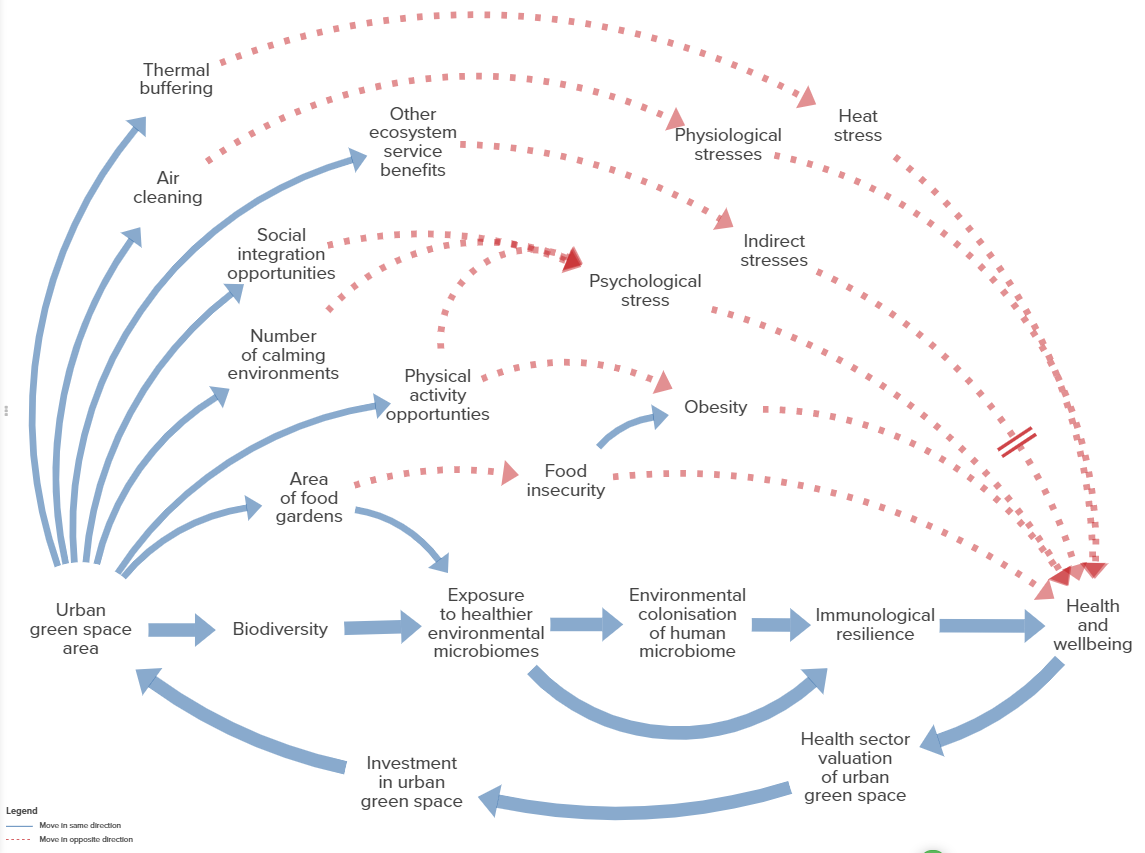
\includegraphics[width=\linewidth]{./figures/HUMI.png}
	\caption[Healthy Urban Microbiome Initiative][6pt]{Causal loop diagram pulled together through extensive consultation with a large group of Australian researchers in Adelaide (Source~\href{https://kumu.io/chrisskelly/humi}{Kumu}).}
	\label{fig:humi}
\end{figure*}



\section{Social Network Modelling for Outbreak Response}
\begin{description}
	\item[What?] Multi-dataset visualisation of potential transmission networks in the Dorset system using a Kumu.io. These visualisations are updated every day and processed using Python scripts (Figure~\ref{fig:socialnetwork}).
	\item[Why?] So that analysts could spend more time looking for insights and less time managing spreadsheets and other data sets in order to support local contact tracing and settings assessment.
	\item[So what?] Reduces analyst time and cost, improves speed of data processing and aids insight development and sharing.
	\item[Insight?] Even 10,000+ data elements and relationships can be explored in minutes in this form and it demonstrates how we can truly extract value from working more closely with Local Public Health Intelligence. PHE data sets, merged with local data sets and explored in KUMU.io after formatting. Almost all of this processing done without analyst intervention.
\end{description}

\begin{figure*}[h]
	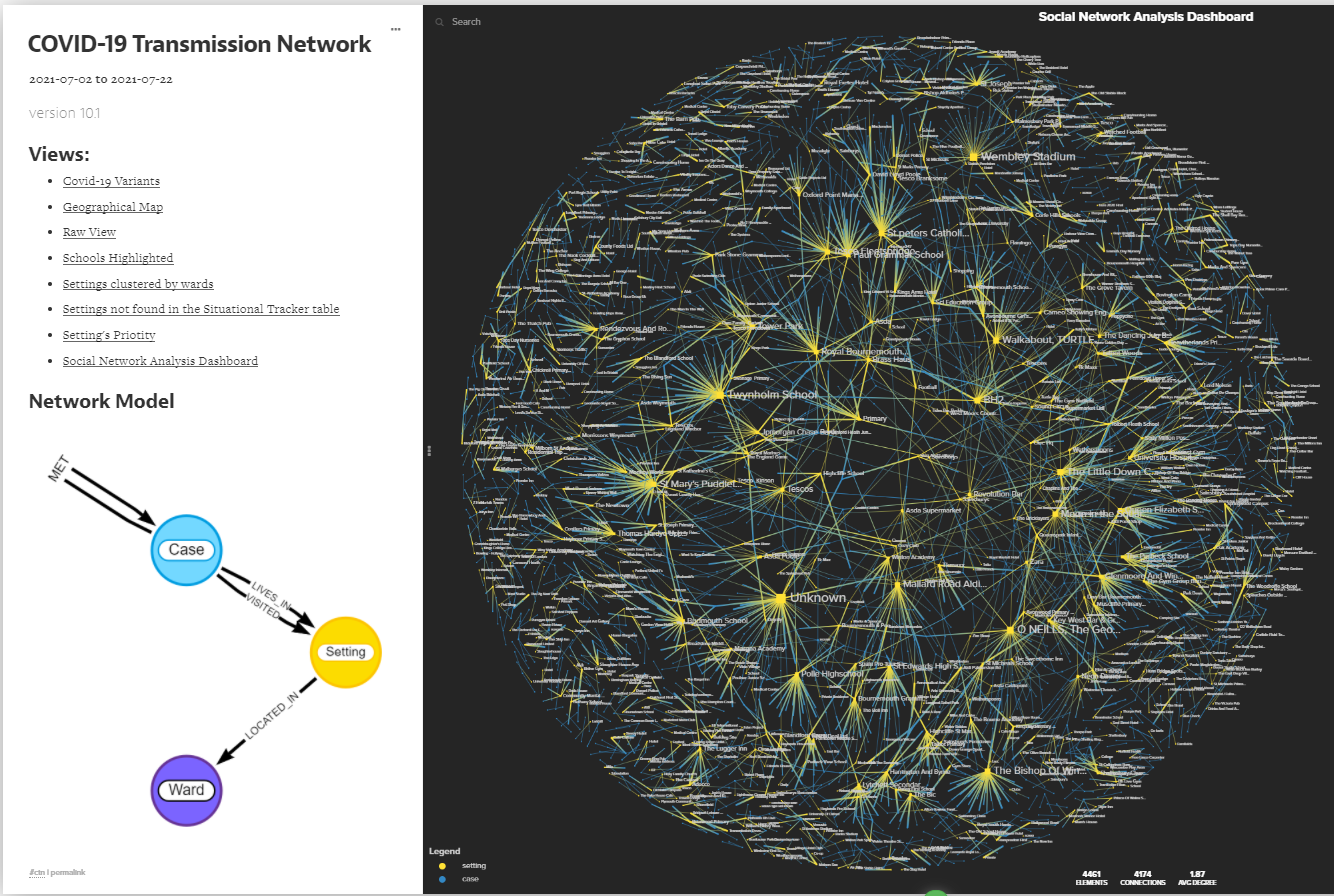
\includegraphics[width=\linewidth]{./figures/Covid19 Social Networks.png}
	\caption[Double Diamond Design Process][6pt]{This is the interface of my copy of a Covid-19 SEIR (Susceptible-Exposed-Infected-Recovered) model developed for Public Health Dorset by (Source~\href{https://www.tanzo.org/}{Tanzo Creative} (Source~\href{https://insightmaker.com/insight/3aozzaFwITwi2Cn6ewR5Wj/Clone-of-Infectious-Disease-Model-Version-4-0}{Insight Maker}). \newthought{Must clear with SC -- PHD DPH Before sharing}Covid-19 Transmission Network (No link as this is sensitive data, but demonstration of site possible with site owner permission).}
	\label{fig:socialnetwork}
\end{figure*}


\section{Systems-Based Healthy Places Scenario Planning}

\begin{description}
	\item[What?] Workshop with senior leaders from across the Dorset health system to identify strategies to take Dorset towards a future of ‘healthy places’
	\item[Why?] Dorset is already seen as wonderful and beautiful landscape that people want to live, work and visit in. However, rarely to people from all walks of the health system consider its health giving potential.
	\item[So what?] Environment is a key component of the ‘wider determinants of health. In the context of health improvement, Dorset’s health places can be viewed as health assets.
	\item[Insight?] The highest ranked strategy for using Dorset’s ‘green’ assets for health improvement was to align population health priorities with political priorities.
\end{description}

\href{https://www.publichealthdorset.org.uk/blogs/the-future-of-healthy-places-developing-futures-strategies.aspx}{The future of ‘healthy places’ — Developing futures strategies}

Is it possible for a group of colleagues to get together, develop a vision of what we want our future to look like AND then actually develop strategies to work towards it?

(Table~\ref{tab:contrasting}).

\begin{table}[h]
	%\resizebox{\textwidth}{!}{
	\begin{center}
		\footnotesize%
		\begin{tabularx}{\linewidth}{p{0.04\linewidth} p{0.135\linewidth} p{0.275\linewidth} p{0.045\linewidth} p{0.35\linewidth}}
			\toprule
			Rank & Focus & Proposed Strategy & Votes & Relevant Work Underway \\
			\midrule
			\multirow{2}{*}{1} & \multirow{2}{\hsize}{Political priorities} & \multirow{2}{\hsize}{Align population health and political priorities} & \multirow{2}{*}{24} & Systems working approach\vspace{0.5\baselineskip} \\
			& & & & Narrative capacity developed with local university media faculty input\vspace{\baselineskip}\\
			
			\multirow{3}{*}{2} & \multirow{3}{\hsize}{Natural Environments} & \multirow{3}{\hsize}{Maximise opportunities from natural environments in local spaces by evaluating health impacts} & \multirow{3}{*}{16} & Public health programme evaluation effort\vspace{0.5\baselineskip} \\
			& & & & System working approach\vspace{0.5\baselineskip} \\
			& & & & Healthy places programme\vspace{\baselineskip} \\
			
			\multirow{2}{*}{3} & \multirow{2}{\hsize}{Active Travel} & \multirow{2}{\hsize}{Increase active travel opportunities as a key element of all travel planning} & \multirow{2}{*}{13} & Systems working approach\vspace{0.5\baselineskip} \\
			& & & & Quantifying accessibility to green space project\vspace{\baselineskip} \\

			\multirow{2}{*}{4} & \multirow{2}{\hsize}{Volunteer resource} & \multirow{2}{\hsize}{Older population is a rich source of skill and experience that could become a major volunteer resource} & \multirow{2}{*}{12} & Prevention at scale – aging well programme\vspace{0.5\baselineskip} \\			
			& & & & System working approach\vspace{0.5\baselineskip} \\
			& & & & Locality working programme\vspace{0.5\baselineskip} \\
			& & & & Health Champions Project\vspace{\baselineskip} \\

			\multirow{2}{*}{4} & \multirow{2}{\hsize}{Sustainable building strategy} & \multirow{2}{\hsize}{Develop a sustainable building strategy (Healthy green developments in partnership)} & \multirow{2}{*}{12} & Healthy places programme\vspace{0.5\baselineskip} \\			
			& & & & Spatial planning development project\vspace{0.5\baselineskip} \\
			& & & & System working approach\vspace{0.5\baselineskip} \\

			\bottomrule
		\end{tabularx}
	\end{center}
	\caption{A subset of the top proposed strategies that senior leaders within the Dorset health system identified during a day-long workshop – a first introduction to futures thinking for the vast majority of participants.}
	\label{tab:contrasting}
\end{table}

\section{Systems-Based Horizon Scanning With Machine Learning Tools}

\begin{description}
	\item[What?] The use of ShapingTomorrow’s AI to scan the horizon has radically changed the process and effort required for organisations to identify trends and weak signals. Public Health Dorset created its own ShapingTomorrow website (Figure~\ref{fig:shapingtomorrow}).
	\item[Why?] There were a number of futures thinking projects that the analyst team felt would contribute to the intelligence and insight programme.
	\item[So what?] With a relatively small team, it was impossible to dedicate the resources to horizon scanning that were needed to be able to produce regular reporting. With AI – horizon scanning is within reach.
	\item[Insight?] Combining horizon scanning with AI and associated data analytics might be a game changer in terms of facilitating more meaningful futures thinking in organisations.
\end{description}

The Future of Healthy Places — a first glimpse…

Are you interested in working towards a future that has healthier places to live, work and learn? If you are, read on. We are using futures studies methods to envision what that future might look like, and my colleagues and I will use this blog to share our insights.

The future of Healthy Places -- Urban Green Space

The first point to make is that research examining the relationship between proximity to well managed urban green space and good health is very consistent – green space in urban environments benefits a population’s health in multiple ways. Not just in urban environments, that’s what we are interested in here, but natural landscapes provide essential ecosystem services from catchment level through to global scale services. Nature is good. Many of us like to wander in green fields and forests when we get the chance – it makes us feel good. Most people get that, but there’s more.

The future of ‘healthy places’ -- Global Warming and Population Ageing

This is a ‘futures’ story about Global Warming and Population Ageing, two global mega trends, and their likely impact Across Dorset, Bournemouth and Poole. We took a small peak into the future and this is what we saw.

\begin{figure*}[h]
	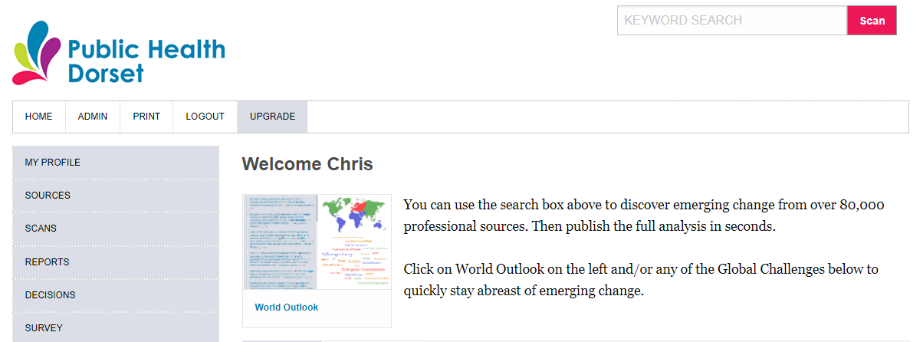
\includegraphics[width=\linewidth]{./figures/ShapingTomorrow.png}
	\caption[Shaping Tomorrow][6pt]{Shaping Tomorrow is an AI horizon scanning tool used to identify what the experts are saying about the future  (\href{https://shapingtomorrow.com}{Shaping Tomorrow Maker}).}
	\label{fig:shapingtomorrow}
\end{figure*}


\section{Imagining A New More Resilient Public Health}
\begin{description}
	\item[What?] The UNFCCC set up a new programme called Resilience Frontiers in 2019 with the express purpose to create “disruption” around how we think about the future of climate change adaptation.
	\item[Why?] Time is running out. The climate emergency is upon us, climate mitigation is not working, and we will be unable to avoid major, maybe catastrophic climatic changes. New thinking is required.
	\item[So what?] They have created eight pathways through which to focus thinking, innovation and the development of new adaptions strategies. Pathway 6. Optimising future health and wellbeing using a holistic and ecosystem approach [Pathway Lead is Dr Chris Skelly, UK]. This is health improvement.
	\item[Insight?] description
\end{description}

Resilience Frontiers was initiated at the Songdo, South Korean futuring event and I wrote a blog a day over the 5-day event, setting out the approach taken at this event.

Resilience Frontiers: Day 1 — Probable Futures. I’m participating in a United Nations Framework Convention on Climate Change (UNFCCC) sponsored event in Song-do, South Korea this week. As part of a larger event on Adaptation to Climate Change, this Resilience Frontiers event, is a five day futuring…

Resilience Frontiers: Day 2 — Desired Futures. Sounds like a population health challenge! The day began with a restatement of the challenge involved in building resilience in the face of climate change; it will be a very familiar problem to those of you working in Public Health…

Resilience Frontiers: Day 3 — Strange Futures. “Never doubt that a small group of thoughtful, committed citizens can change the world; indeed, it’s the only thing that ever has.” Margret Mead Day 1 — Probable Futures — identify and describe what we think is most likely…

Resilience Frontiers: Day 4 — Group Moonshot. We had an incredibly long day today or so it seemed. Group work is exhausting, but satisfying when the discussions are interesting and complex. We followed the same process for making a Moonshot as we did on Day 2…

Resilience Frontiers: Day 5 — Conceiving Policy. Thoughts on the Week This was a long and often intense week — as only these types of events can be. The reality of actually gathering together 125 people from a variety of professional, cultural and demographic backgrounds…

Resilience Frontiers 2021-2030

Each of the eight RF Pathways are to chart their own way through the development of new ideas and the development of innovative adaption projects and strategies.


\section{Public Health Intervention Planning Tool}
\begin{description}
	\item[What?] A generic intervention planning tool for public health colleagues. Captures the dynamics of any intervention based on three critical elements: intervention reach, intervention compliance and intervention efficacy. It allows local systems to tailor costs and population to their situation (Figure~\ref{fig:intervention}).
	\item[Why?] There seems to be a wide-spread lack of appreciation amongst public health colleagues on the value of using these three elements in the management and evaluation of intervention programmes.
	\item[So what?] Knowledge to action. If we want to improve public health interventions, we must develop a better shared-understanding of why some interventions are more successful than others.
	\item[Insight?] High efficacy interventions do not necessarily make the best public health interventions. ‘Reach’ and ‘compliance’ are intervention elements that are determined by the health system and its users, and we need to actively incorporate this into our knowledge to action work.
\end{description}

\marginnote{Blog: \href{https://www.publichealthdorset.org.uk/blogs/future-of-public-health-intervention-three-cold-hard-numbers.aspx}{Future of Public Health Intervention: Three Cold Hard Numbers}
}

People are full of ideas, but how do we harness discussions about population health interventions and move them rapidly into real-world thinking and planning.

\begin{figure*}[h]
	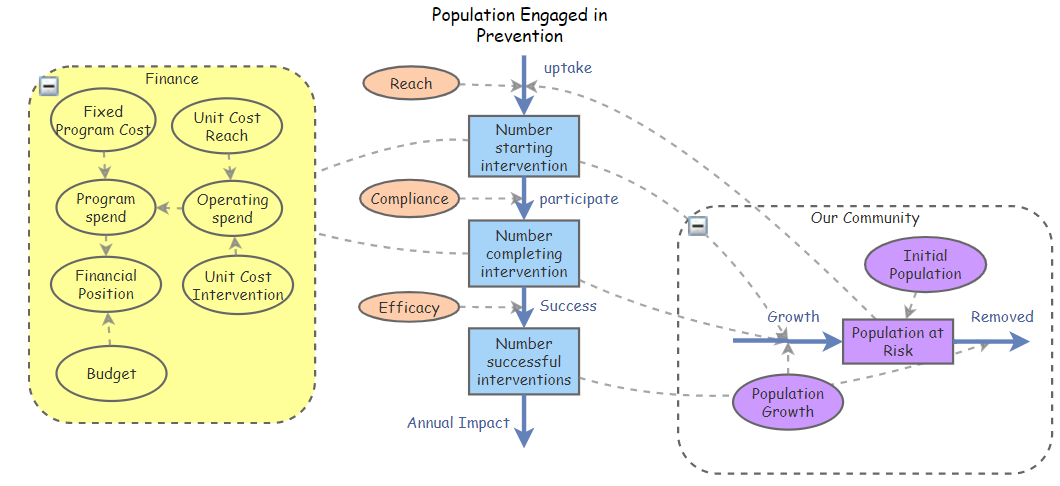
\includegraphics[width=\linewidth]{./figures/Intervention Planning Tool.png}
	\caption[Double Diamond Design Process][6pt]{This is the interface of my copy of a CVD Prevention Model that I modified from a model developed  after~\href{https://www.tanzo.org/}{Tanzo Creative} (\href{https://insightmaker.com/insight/1Oqiscp4ZdbYBaElk4Qq9W/CVD-System-Dynamics-Model-V1-1}{Insight Maker}).}
	\label{fig:intervention}
\end{figure*}


\section{Covid-19 Response Decision-Making}

\begin{description}
	\item[What?] In April 2020 Dorset Public Health commissioned a systems model to capture what was known about SARS-CoV-2 community transmission in order to be able to simulate the Dorset situation (Figure ~\ref{fig:seir}).
	\item[Why?] There is very little epidemiological knowledge within the Dorset system, especially in infectious disease. We believe the model as a reservoir of what we know and understand about the nature of this disease, would be an engaging tool to develop a better shared-understanding.
	\item[So what?] Knowledge to action. We will be conducting a post-hoc evaluation, but I feel that introducing this model into the Dorset ICS’s ‘Covid-19 epicell’ improved the quality of discussion, which in turn improved decision-making. This was our objective and we will attempt to evaluate this later in the year.
	\item[Insight?] Providing colleagues with recent trend data (deaths, cases, hospitalisations) provoked the question – “so what will happen next?” Providing colleagues with a model projection provoked the question – “how do we know this is right?” The first response takes us to more data. The second response takes us straight into a conversation about the dynamics of Covid-19 in our community.
\end{description}

\begin{figure*}[h]
	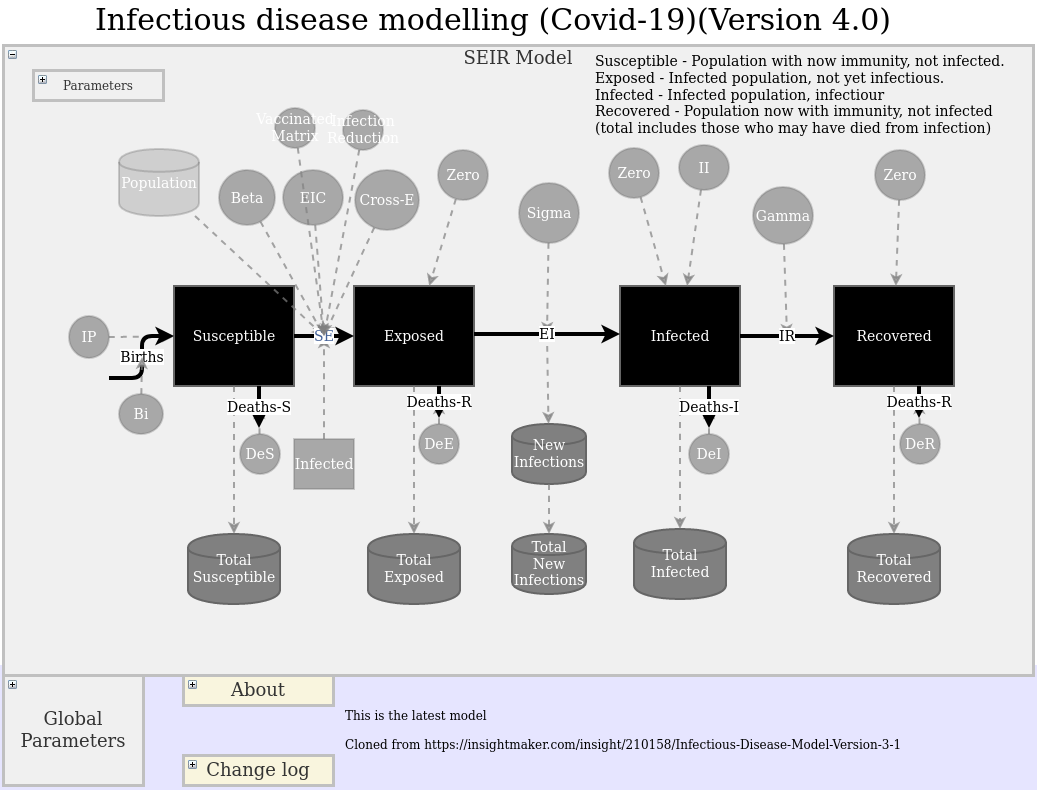
\includegraphics[width=\linewidth]{./figures/Covid19 SEIR Model.png}
	\caption[Double Diamond Design Process][6pt]{This is the interface of my copy of a Covid-19 SEIR (Susceptible-Exposed-Infected-Recovered) model developed for Public Health Dorset by (Source~\href{https://www.tanzo.org/}{Tanzo Creative} (Source~\href{https://insightmaker.com/insight/3aozzaFwITwi2Cn6ewR5Wj/Clone-of-Infectious-Disease-Model-Version-4-0}{Insight Maker}).}
	\label{fig:seir}
\end{figure*}


\section{Cardio-Vascular Disease Prevention}

\begin{description}
	\item[What?] We have constructed a systems model to simulate the impact of CVD prevention in local systems to support PHE colleagues in their renewed push for greater knowledge to action (Figure~\ref{fig:CVD}).
	\item[Why?] A systems model is a tool that can be used to capture knowledge and data into an interactive process of ‘what ifs’, that diverse groups of colleagues from an ICS can engage with each other to understand the behaviour of their local population and health system under various interventions.
	\item[So what?] Knowledge to action. Systems thinking and modelling provides a coherent pathway towards more informed decision-making through which there is improved shared-understanding of the challenges across the ICS. This will be the model used in our system modelling training course.
	\item[Insight?] Initial engagement with PHE staff in the CVD Prevention area indicates that they really appreciate what this type of modelling does and see a role for it within their programme.
\end{description}

\begin{figure*}[h]
	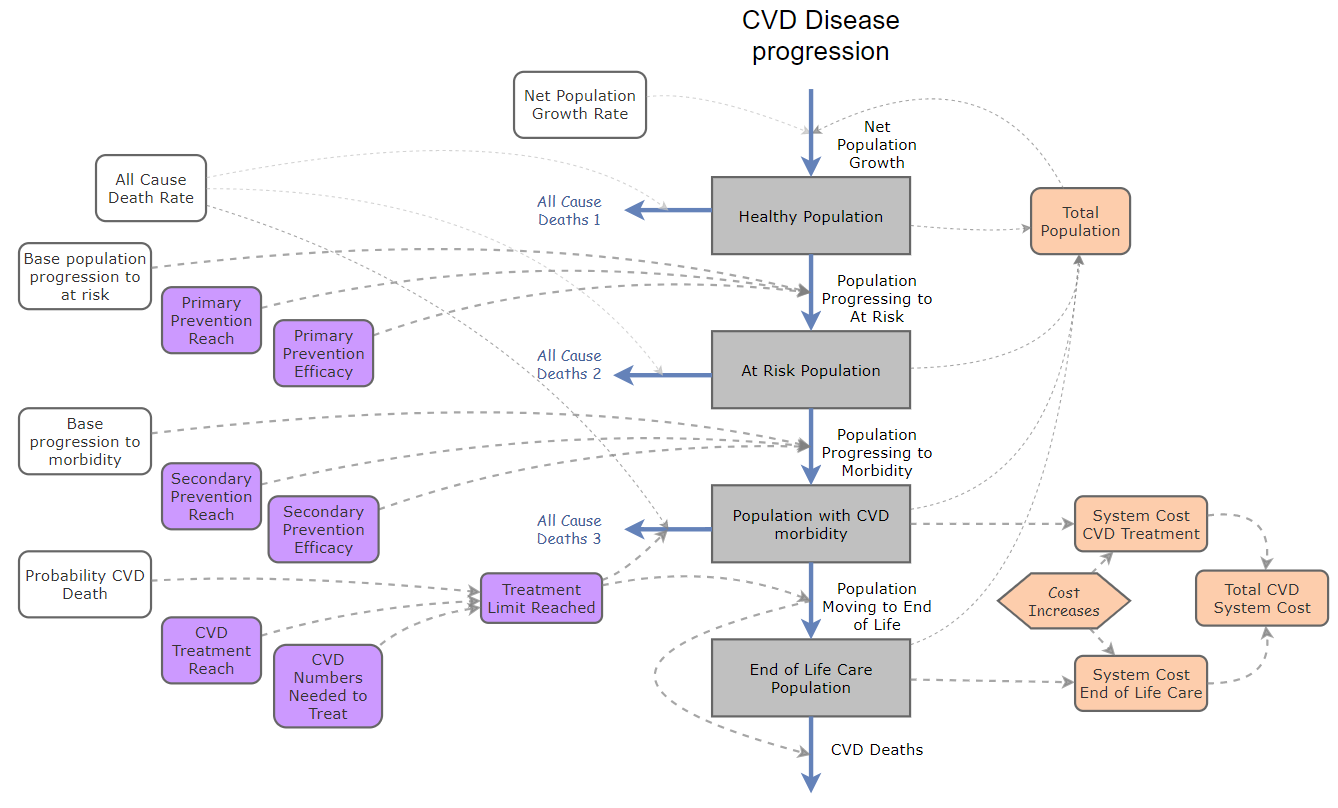
\includegraphics[width=\linewidth]{./figures/CVD Model.png}
	\caption[Double Diamond Design Process][6pt]{This is the interface of my copy of a CVD Prevention Model that I modified from a model developed by (Source: After~\href{https://www.tanzo.org/}{Tanzo Creative} (Source~\href{https://insightmaker.com/insight/1Oqiscp4ZdbYBaElk4Qq9W/CVD-System-Dynamics-Model-V1-1}{Insight Maker}).}
	\label{fig:CVD}
\end{figure*}


%  The back matter contains appendices, 
%  bibliographies, indices, glossaries, etc.
\backmatter
\bibliography{systems_book}
\bibliographystyle{plainnat}
\printindex


\end{document}

